%\documentclass[MScThesis,twoside]{sharifthesis}
%\documentclass[MScThesis,oneside]{sharifthesis}
\documentclass[MScThesis,twoside]{sharifthesis}
%\documentclass[PhDThesis,oneside]{sharifthesis}
%\documentclass[PhDProposal,twoside]{sharifthesis}
%\documentclass[PhDProposal,oneside]{sharifthesis}

%\def\enSubject{Master of Science Thesis (Information Technology Major), Computer Engineering Department, Sharif University of Technology, Tehran, I. R. Iran}
\def\enSubject{Doctor of Philosophy Thesis (Information Technology Major), Computer Engineering Department, Sharif University of Technology, Tehran, I. R. Iran}
%\def\enSubject{Doctor of Philosophy Research Proposal (Information Technology Major), Computer Engineering Department, Sharif University of Technology, Tehran, I. R. Iran}

%do not use newline command (\\) in following definition
\def\enTitle{Title of thesis}
%if title is long and requires to be splitted in two lines, uncomment following two definitions and split title at appropriate location (you should uncomment two corresponding lines in the rest of this file too)
%\def\enTitleLineOne{First line of the long title}
%\def\enTitleLineTwo{and its continuation on the second line}
\def\enAuthor{‌Behnam Momeni}
\def\enKeywords{First Key Word, Second Key Word, Final Key Word}


 \usepackage{color}

\usepackage{amssymb}
\usepackage{mathrsfs}
\usepackage{algorithmicx}
\usepackage{graphicx}
\usepackage{multirow}
\usepackage{comment}
\usepackage[style=ieee,backend=biber]{biblatex}
\newcommand{\bibliographytitle}{\rl{کتاب‌نامه}}
\usepackage{paralist}
\usepackage{textcomp}
\usepackage{ctable}% for tables (it provides table-notes and imports booktabs package too)
\usepackage[xindy]{glossaries}
\newcounter{tablerow}
\renewcommand{\arraystretch}{1.5}
\usepackage{cleveref}
\usepackage{csvsimple}
\usepackage{longtable}
\usepackage{color}
\usepackage{setspace}
\usepackage[table]{xcolor}  
\usepackage{tablefootnote}
 

\newcommand{\crefrangeconjunction}{--}
\crefformat{tablerow}{#2#1#3}
\crefmultiformat{tablerow}{#2#1#3}%
{ و~#2#1#3}%
{, #2#1#3}%
{ و~#2#1#3}
\crefformat{section}{#2#1#3}
\crefmultiformat{section}{#2#1#3}%
{ و~#2#1#3}%
{, #2#1#3}%
{ و~#2#1#3}



\input{general/translitaration}

\نوواژه[کلید]{نمونه}{Example}
\نوواژه{خودگرد}{Automata}
\نوواژه{قالب}{Template}
\نوواژه{پوشه}{Folder}
\نوواژه{پرونده}{File}
\نوواژه{پروندهی}{File}
\نوواژه{بسته}{Package}
\نوواژه{سامانه‌ی کنترل نسخه}{Version Control System}
\نوواژه{قطعه}{Component}
\نوواژه{خطا‌خیزی}{Bug-proneness}
\نوواژه{ماتریس درهم‌ریختگی}{Confusion Matrix}
\نوواژه{معیارهای محصول}{Product Metrics}
\نوواژه{فرض زمینه‌ای}{Ground Assumption} 
\نوواژه{جریان کنترلی}{Control Flow} 
\نوواژه{پیچیدگی حلقوی}{Cyclomatic Complexity}
\نوواژه{همبستگی}{Cohesion} 
\نوواژه{زوجیت}{Coupling}
\نوواژه{بازآرایی کد}{Refactoring} 
\نوواژه{ثبت}{Commit}
\نوواژه{شهرت}{Popularity}
\نوواژه{بررسی قاعده‌مند}{Systematic Review}
\نوواژه{تکرار}{Iteration} 
\نوواژه{انتشار}{Release} 
\نوواژه{جهت‌گیری}{Bias}
\نوواژه{نیمه-نظارتی}{Semi-Supervised}
\نوواژه{آماره‌های توصیفی}{Descriptive Statistics} 
\نوواژه{درخت تصمیم}{Decision Tree}
\نوواژه{دسته‌بندی}{Classification} 
\نوواژه{اشکال زدایی}{Debugging} 
\نوواژه{اندازه‌گیری  وکالتی}{Proxy Measurement}
\نوواژه{امتیاز جهش }{Mutation Score}
\نوواژه{جهش‌یافته}{Mutant}
\نوواژه{شرط شاخه}{Branch Condition}
\نوواژه{مشکوک بودن}{Suspiciousness}
\نوواژه{منسوخ}{Obsolete}
\نوواژه{ارزیابی میان دسته‌ای}{Cross-validation}
\نوواژه{توضیح}{Comment}
\نوواژه{مستند‌جاوا}{Javadoc}
\نوواژه{پیکربندی}{Configuration}
\نوواژه{متن-باز}{Open-source}
\نوواژه{چهارچوب}{Framework}
\نوواژه{وابستگی}{Dependency}
\نوواژه{خط دستور}{Command line}
\نوواژه{افزونه}{Plugin}
\نوواژه{کارایی}{Performance}
\نوواژه{عمومی}{Generic}
\نوواژه{سبک‌وزن}{Lightweight}
\نوواژه{حاشیه‌نویسی شده}{Annotated}
\نوواژه{ورودی/خروجی}{Input/Output (IO)}
\نوواژه{پوشه‌ی کاری}{Working Directory}
\نوواژه{ماشین مجازی جاوا}{Java Virtual Machine}
\نوواژه{فراداده}{Metadata}
\نوواژه{زمان خروج}{Timeout}
\نوواژه{زباله‌روب}{Grabage Collector}
\نوواژه{متعادل}{Balanced}
\نوواژه{فضای ویژگی}{Feature Space}
\نوواژه{ابرصفحه}{Hyperplane}
\نوواژه{مورد آزمون}{Test Case}
\نوواژه{انقیاد}{Bind} 
\نوواژه{ساخت}{Build}


\newcommand{\myrotate}[3][]{\rotatebox{90}{\parbox[c][#1]{#2}{\centering\arraybackslash\rl{#3}}}}
\newcommand{\multilinescell}[2][c]{\begin{tabular}[#1]{@{}c@{}}#2\end{tabular}}
\newcommand{\twolinescell}[3][c]{\multilinescell[#1]{#2\\#3}}
\newcommand{\itemrl}[1][]{\item[\rl{#1}]}
\eqcommand{چرخش}{myrotate}
\eqcommand{سلولچندخطی}{multilinescell}
\eqcommand{سلول‌دوخطی}{twolinescell}
\eqcommand{فقره‌راست}{itemrl}



\newcommand{\Eqn}[1]%
{فرمول~(#1) }
\newcommand{\Eqns}[1]%
{فرمول‌های~(#1) }

\eqcommand{فرمول}{Eqn}
\eqcommand{فرمولهای}{Eqns}

\فرمان‌نو{\نگا}{ن.بـ.}
\فرمان‌نو{\نگاص}[1]{\نگا{} صفحه‌ی~\رجوع‌صفحه{#1}}
\فرمان‌نو{\آیم}[1][$i$]%
{#1اُم}

\newcolumntype{C}[1]{>{\centering\arraybackslash}m{#1}}

\فرمان‌نو{\نامک}[1]{%
\fcolorbox{red}{yellow}{\begin{minipage}{\textwidth}#1\end{minipage}}}

\newcommand{\tobewritten}[1]{\نامک{%
این جعبه، باید با متن متناظر با \چر{#1} جای‌گزین گردد.

برای دریافتن معنی \چر{#1} به پرونده‌ی \چر{TODO} نگاه کنید.
}}

\graphicspath{{img/}}% tell tex engine address of folder containing your pictures


\hypersetup{
	pdftitle = {\enTitle},
	pdfauthor = {\enAuthor},
	pdfsubject = {\enSubject},
	pdfkeywords = {\enKeywords}
}



\renewcommand{\lstlistingname}{\rl{قطعه کد}}

\raggedbottom

\definecolor{codegreen}{rgb}{0,0.6,0}
\definecolor{codegray}{rgb}{0.5,0.5,0.5}
\definecolor{codepurple}{rgb}{0.58,0,0.82}
\definecolor{backcolour}{rgb}{0.95,0.95,0.92}
\definecolor{codeblue}{rgb}{0.11,0.191,0.80}

\lstdefinestyle{mystyle}{
	backgroundcolor=\color{backcolour},   
	commentstyle=\color{codegreen},
	keywordstyle=\color{magenta},
	numberstyle=\tiny\color{codegray},
	stringstyle=\color{codepurple},
	basicstyle=\footnotesize,
	breakatwhitespace=false,         
	breaklines=true,                 
	captionpos=b,                    
	keepspaces=true,                 
	numbers=left,                    
	numbersep=5pt,                  
	showspaces=false,                
	showstringspaces=false,
	showtabs=false,                  
	tabsize=2
}

\lstset{style=mystyle}

\fontdimen2\font=3pt

\renewcommand{\autodot}{} %remove last dots from title




%\addbibresource{resources/resources.bib}
\bibliography{resources/resources.bib}

\newcommand{\faKeywords}{واژه‌ی کلیدی نخست،
واژه‌ی کلیدی دوم،
واژه‌ی کلیدی پایانی}
\eqcommand{واژه‌های‌کلیدی}{faKeywords}
\آرم{\درج‌تصویر[scale=.7]{logo}}
\تاریخ{شهریور 1397}
%در دستور زیر، از \\ استفاده نکنید
\عنوان{مدل پیش بینی خطا مبتنی بر معیارهای جهش}
%اگر عنوان طولانی بوده (و در عنوان انگلیسی از دو خظ استفاده شده) باید دو خط زیر از کامنت خارج و دو خط عنوان توسط آن‌ها تعریف گردد.
%\عنوانخطیک{خط نخست عنوان طولانی}
%\عنوانخطدو{و ادامه‌ی آن در خط دوم}
\نویسنده{علی محبی   \newline}
\دانشگاه{{\نستعلیق\درشت‌تر دانشگاه صنعتی شریف %
\\[0.6cm]}
دانشکده‌ی مهندسی کامپیوتر}
\دانشگاه‌عادی{دانشگاه صنعتی شریف\\
دانشکده‌ی مهندسی کامپیوتر}
\موضوع{مهندسی نرم‌افزار}
\استادراهنما{دکتر حسن میریان}
%اگر استاد مشاور دارید، خط زیر را از comment خارج کنید
%همچنین، فراموش نکنید در آخر این پرونده، اطلاعات انگلیسی معادل این دستورها را هم پر کنید
%\استادمشاور{دکتر <نام استاد مشاور>}

\newcommand{\efootnote}[1]{\footnote{\lr{#1}}}
\newcommand{\ecfootnote}[1]{}


% ================ Correct hyphenations ================
\hyphenation{test}


\makeglossaries
%\includeonly{related_works/related_works}
%\includeonly{evaluation/evaluation}

% ===== DEPRACATED AREA =====
% Following commands are provided to make older documents compilable.
% These commands are depracated and should not be used in new documents.
\newcommand{\ترجمه‌ج}[2]
{\ترجمه[#1‌ها]{#1}{#2}}
\newcommand{\ترجمه‌جمع}[3]
{\ترجمه[#3]{#1}{#2}}
\newcommand{\برگردان}[3]
{\ترجمه{#1}{#3}\زیرنویس{#2}}
\eqcommand{اسم}
{نام}
% ===== END OF DEPRACATED AREA =====

\شروع{نوشتار}


\newcommand{\StartDocument}{\frontmatter \baselineskip1.2\baselineskip \pagestyle{empty} \null \vfill
\شروع{وسط‌چین}
{\نستعلیق‌درشت بسم اللّه الرّحمن الرّحیم}
\پایان{وسط‌چین}
\vfill}

%the initial title is supposed to be printed on the cover.
%for non final version, you can leave following commands as is to create only one title page (printed on paper)
%for final version you need to swap folowing commented/uncommented makethesistitle commands to achieve this order: title on the cover THEN in the name of god page THEN another title page but this time printed on paper
\makethesistitle
\StartDocument
%\makethesistitle

\pagestyle{plain.ThesisPagestyle}
% following parts are not required in PhD proposal and should be removed. BEGIN OF COMMENT FOR PhD Proposal........
%صفحه‌ی تصویب در پیشنهاد پژوهشی وجود ندارد.
\شروع{تصویب}
%خط‌های زیر در صورت نبود استاد مدعو comment شوند
\داور{استاد مدعو}{دکتر <نام استاد مدعو ۱>}
\داور{استاد مدعو}{دکتر <نام استاد مدعو ۲>}
\پایان{تصویب}
\newpage
% برگه‌ی اظهارنامه را که به صورت خالی با دستور زیر ایجاد می‌شود، پس از چاپ با خودکار پر کرده و امضاء کنید.
\اظهارنامه{رساله}{دکتری}
%\اظهارنامه{پایان‌نامه}{کارشناسی~ارشد}
\newpage

\تقدیم{\درشت تقدیم به ...؛   صفحه‌ی تقدیم اختیاری است.}

\setlength{\baselineskip}{0.9cm}
\begin{comment}
\فصل*{پیش‌گفتار}
\thispagestyle{plain.ThesisPagestyle}
پیشگفتار اختیاری است. در صورت تمایل به نگارش پیش‌گفتار، محیط کامنت که آن را دربرگرفته باید حذف شود.
\end{comment}

\شروع{قدردانی}
صفحه‌ی قدردانی. این صفحه اختیاری بوده و می‌توانید آن را حذف کنید. برای این کار کافی است محیط قدردانی در پرونده‌ی تِک را حذف کنید. متداول است که در این صفحه از خانواده، استادها و همکارهای خود قدردانی نمایید.
\پایان{قدردانی}
% END OF COMMENT FOR PhD Proposal.

\شروع{چکیده}{\واژه‌های‌کلیدی}
% abstract ...
% write it at the end...
%persian abstract

 توسعه‌دهندگان نرم‌افزار از طریق گزارش خطا در سیستم­‌های ردگیری خطا و یا شکست در آزمون نرم‌‌افزار متوجه حضور خطا می‌شوند و پس از آن به جستجوی محل خطا و درک مشکل  نرم‌‌افزار می‌‌پردازند. کشف زود هنگام خطاها موجب صرفه‌‌جویی در زمان و هزینه می­‌شود و فرآیند اشکال زدایی را تسهیل می‌­بخشد. ابزارهای آماری نوین امکان ساخت و بهره‌‌برداری از مدل‌های پیش‌بینی را فراهم می‌سازند. اصلی‌ترین جزء مدل‌های پیش‌بینی، معیارهای نرم‌افزار می‌باشد و با به کارگیری معیارهای نوین و موثر می‌توان به مدل‌های کاراتر دست پیدا کرد. در این پژوهش از معیارهای فرآیند و معیارهایی که بر اساس تحلیل جهش ساخته شده‌اند استفاده شده عملکرد مدل‌های حاصل ارزیابی شده‌اند. علاوه بر بکارگیری معیارهای جهش در کنار معیارهای فرآیند دو دسته معیار جدید به نام‌های معیارهای \موکد{فرآیند مبتنی بر جهش } و معیارهای \موکد{ترکیبی جهش-فرآیند} نیز جهت به کارگیری در ساخت مدل‌های پیش‌بینی معرفی شده‌اند. نتایج ارزیابی نشان می‌دهد معیارهای جهش می‌تواند به قدرت پیش‌بینی معیارهای فرآیند بیافزاید. معیارهای فرآیند مبتنی بر جهش علارغم داشتن قدرت پیش‌بینی بهتر از معیارهای جهش عمل نمی‌کنند. همچینین معیارهای ترکیبی جهش-فرآیند بهبود قابل توجهی را در عملکرد مدل‌های پیش بینی ایجاد می‌کنند. 

\پایان{چکیده}


\setlength{\baselineskip}{0.9cm}
\pagenumbering{tartibi}\tableofcontents\listoftables\listoffigures
%list of abbreviations may be added here...


\PrepareForMainContent
\pagestyle{ThesisPagestyle}
%	In the name of GOD

	
\chapter{سرآغاز}
\baselineskip=.95cm
\برچسب{chap:intro}
امروزه سامانه‌های نرم‌افزاری بسیار فراگیر شده‌اند و زندگی روزمره را تحت تاثیر قرار داده‌اند. در نتیجه کاربران کیفیت نرم‌افزار بالایی را تقاضا می‌کنند. کشف و برطرف کردن خطاها پرهزینه است و مدل‌های پیش‌بینی خطا  از طریق اولویت‌دهی به فعالیت‌های تضمین کیفیت موجب افزایش بازدهی می‌گردند. پیش‌بینی خطا از سال ۱۹۹۲ تا کنون یک زمینه‌ی فعال تحقیقاتی بوده است. محققان همواره به دنبال روش‌هایی بوده‌اند که پیش‌بینی خطا را با کیفیت بهتری انجام دهند و یا دامنه‌ی کاربرد آن را گسترش بخشند. 

به  منظور افزایش کارایی پیش‌بینی‌خطا محققان معیارهای نوینی را ارائه داده‌اند\cite{bacchelli2010popular}، سعی داشته‌اند محدودیت‌های یادگیری ماشین را تقلیل بخشند\cite{limsettho2018cross} و یا روش‌های بروزتری را به منظور \واژه{دسته‌بندی} به کار گیرند\cite{chen2016software}. 

\section{ تعاریف مقدماتی}
\label{sec:terms}
در این قسمت چند اصطلاح رایج در مبحث پیش‌بینی‌ خطا و مورد استفاده در پایان‌نامه نوشته شده است.
\begin{itemize}
	\item 
	\واژه{مورد آزمون}: \\
	یک مورد آزمون متشکل است از مقادیر ورودی‌های آزمون، نتایج مورد انتظار که با اجرای برنامه تحت آزمون یک یا چند عملکرد آنرا ارزیابی می‌کند. 
	\item
	\واژه{سامانه‌ی کنترل نسخه}:\\
	این سامانه تغییرات اعمال شده بر روی یک یا چندین \واژه{پرونده} را ذخیره می‌کند تا در آینده بتوان یک نسخه‌ی خاص را بازخوانی کرد. 
	\item
	\واژه{ثبت}:\\
	ذخیره‌ی تغییرات ایجاد شده بر روی پرونده‌ها در سامانه‌ی کنترل نسخه‌ را ثبت می‌نامند. یک ثبت را می‌تواند معادل یک نسخه از برنامه در نظر گرفت که البته این نسخه می‌تواند ناکامل باشد.
	\item
	\واژه{انتشار}:\\
	انتشار به معنی توزیع نسخه‌ی نهایی یک نرم‌افزار است که قابل استفاده برای کاربر می‌باشد. یک انتشار ممکن است نسخه‌ای از یک برنامه‌ی جدید باشد و یا ارتقاء یافته‌ی نرم‌افزار موجود باشد. قبل از یک انتشار معمولا به ترتیب نسخه‌های \نام{آلفا}{Alpha} و \نام{بتا}{Beta} توزیع می‌شود. 
	\item
	\واژه{ماتریس درهم‌ریختگی}:\\
	در زمینه‌ی یادگیری ماشین، به خصوص مسئله‌ی دسته‌بندی، ماتریس درهم‌ریختگی یک جدول است که اجازه می‌دهد عملکرد یک الگوریتم تصویر‌سازی گردد. هر سطر از ماتریس نشان دهنده‌ی نمونه‌هایی است که پیش‌بینی شده‌اند در حالی که هر ستون نمونه‌ها در کلاسهای واقعی را نشان می‌دهند(یا بالعکس). این ماتریس با توجه به این واقعیت نامگذاری شده است که  مشخص می‌کند که آیا یک سیستم دو کلاس را با هم اشتباه گرفته است یا خیر. ماتریس درهم ریختگی برای دسته‌بندی دو کلاس فرضی (آ) و (ب) در جدول \ref{tab:confusion-matrix} آمده است. \\
	در این جدول نمونه‌هایی که در دسته‌ی آ قرار می‌گیرند مثبت در نظر گرفته شده‌اند. این ماتریس از چهار عنصر اصلی تشکیل شده است که در زیر شرح داده شده اند. 
	\begin{itemize}
		\item 
		\واژه{مثبت واقعی}: تعداد نمونه‌هایی را نشان می‌دهد که به درستی در دسته‌ی آ پیش‌بینی شده‌اند.
		\item
		\واژه{مثبت اشتباه}: تعداد نمونه‌هایی را نشان می‌دهد که در دسته‌ی آ پیش‌بینی شده‌اند اما در واقع در دسته‌ی ب قرار دارند.
		\item
		\واژه{منفی اشتباه}: تعداد نمونه‌هایی را نشان می‌دهد که در دسته‌ی ب پیش‌بینی شده‌اند اما در واقع در دسته‌ی آ قرار دارند.
		\item
		\واژه{منفی واقعی}: تعداد نمونه‌هایی را نشان می‌دهد که به درستی در دسته‌ی ب پیش‌بینی شده‌اند.
	\end{itemize}
	
\end{itemize}	

\begin{table}[H] 
	\renewcommand*{\arraystretch}{1.5}	
	\centering \caption{ماتریس درهم‌ریختگی}
	\newcolumntype{C}{>{\centering\arraybackslash} m } 
	\label{tab:confusion-matrix}

	\begin{tabular}{|C{2cm}|c|C{3cm}|C{3cm}|}
		
		\cline{3-4}
		\multicolumn{2}{c|}{}
	&	\multicolumn{2}{c|}{دسته‌ی واقعی}
		\\
	
		\cline{3-4}
		\multicolumn{2}{c|}{}
  & دسته‌ی آ  &  	دسته‌ی ب
		\\ \hline
		
		\multirow{2}{*}{\shortstack{
		دسته‌ی\\
			 پیش‌بینی\\
			  شده}
	} \rule{0pt}{6ex}   & 
	
دسته‌ی آ &مثبت واقعی \cellcolor{green!15} &مثبت اشتباه \cellcolor{red!15} 
		\\ \cline{2-4}\rule{0pt}{6ex}  & 

دسته‌ی ب   &منفی اشتباه \cellcolor{red!15}  & منفی واقعی \cellcolor{green!15} 

		\\
		\hline
		
	\end{tabular}
\end{table}

\begin{itemize}
\item
\textbf{اندازه:}
یک مقدار عددی است که نشانگر طول، ابعاد، ظرفیت و یا بزرگی یک صفت از محصول یا فرآیند است.

\item
\textbf{معیار:}
یک اندازه‌گیری عددی مرتبط با  سیستم، محصول و یا فرآیند است که نشان می‌دهد به چه میزان یک صفت داده  شده را دارا می‌باشد. 	معمولا معیارها از ترکیب چند اندازه به دست می‌آیند. 
\end{itemize}


\section{بیان مسئله}
آزمون نرم‌افزار اصلی‌ترین فعالیت تیم  تضمین کیفیت می‌باشد. آزمون نرم‌افزار می‌تواند تا ۵۰ درصد هزینه‌ی تولید نرم‌افزار را به خود اختصاص دهد. هدف از پیش‌بینی خطا افزایش بازدهی این فرآیند می‌باشد. حال با بهبود پیش‌بینی خطا می‌توان به این هدف نزدیکتر شد. به منظور پیش‌بینی خطا معیارهایی  در سطح مورد نظر استخراج می‌گردد. منظور از سطح مورد نظر سطوح مختلف برنامه مانند زیر‌سیستم، \واژه{بسته}، \واژه{پرونده} و تابع می‌باشد. سپس با استفاده از دسته‌بندی، خطادار بودن یا نبودن قطعه‌ی مورد بررسی پیش‌بینی می‌شود. یک دسته از معیارهای مورد استفاده در این زمینه معیارهای فرآیند است و معیارهای جهش نیز به تازگی در این راستا استفاده شده‌اند. این پایان‌نامه قصد دارد تا بررسی کند که معیارهای جهش در کنار فرآیند  چه میزان در پیش‌بینی خطا تاثیر گذار است و همچنین بر اساس مفاهیم تحلیل جهش معیارهای جدیدی ارائه دهد تا پیش‌بینی خطا بهبود یابد. \\

با توجه به اینکه معیارهای جهش به تازگی در پیش‌بینی خطا مورد استفاده قرار گرفته‌اند لازم است تا تحقیقات بیشتری در مورد آنها صورت گیرد و عملکرد آنها از ابعاد مختلف مورد بررسی قرار گیرد. همچنین با بررسی مطالعات پیشین نقاط ضعف و قوت معیارهایی که تا کنون ارائه شده‌اند مورد بررسی قرار می‌گیرد. در این پایان‌نامه عملکرد معیارهای فرآیند و جهش مورد بررسی بیشتری قرار می‌گیرند و با توجه به نقاط ضعف و قدرت معیارهای قبلی، معیارهایی ارائه شده تا بخشی از نقاط ضعف را پوشش دهند و به پیش‌بینی بهتری بیانجامند. 
\section{ساختار پایان‌نامه}

این پایان‌نامه در ۶ فصل تهیه گردیده است. در فصل \ref{chap:survey} به مرور مطالعات پیشین پرداخته می‌شود که در  قسمت \ref{sec:bug-predict}  مباحث مربوط به پیش‌بینی خطا از جمله فرآیند پیش‌بینی، معیارهای ارزیابی، معیارهای پیش‌بینی و مدل‌های پیش‌بینی بررسی می‌شوند. در قسمت \ref{sec:mutation} مباحث مربوط به آزمون جهش بررسی شده‌اند و در قسمت \ref{sec:conclustion} مطالعات مروری جمع‌بندی شده‌اند. در فصل \ref{chap:method} معیارهای مورد استفاده و ارائه شده در این پایان‌نامه معرفی می‌شوند. در فصل \ref{chap:case-study} پنج پروژه‌ی صنعتی مورد مطالعه قرار گرفته‌اند و در فصل \ref{chap:evaluation} معیارها مورد ارزیابی قرار گرفته‌اند. در فصل \ref{chap:future} مباحث مطرح شده در این پایان‌نامه جمع‌بندی شده و کارهای آتی شرح داده شده است. 
	

\chapter{مرور مطالعات پیشین}

\label{chap:survey}

\section{پیش بینی خطا}
\label{sec:bug-predict}
\subsection{فرآیند پیش‌بینی خطا}
\label{subsec:process}
اکثریت پژوهش‌های پیش‌بینی خطا از روش‌های یادگیری ماشین  استفاده کرده‌اند. اولین گام در ساخت مدل پیش‌بینی تولید داده‌هایی با استفاده از آرشیو‌های نرم‌افزاری همانند \واژه[سامانه‌های کنترل نسخه]{سامانه‌ی کنترل نسخه} مانند \نام{گیت}{Git}، سیستم‌های ردگیری مشکلات  مانند جیرا و آرشیو ایمیل‌ها است. هر یک از این داده‌ها بر اساس درشت دانگی پیش‌بینی می‌توانند نمایانگر یک سیستم، یک \واژه[قطعه‌ی]{قطعه} نرم‌افزاری، \واژه{بسته}، فایل کد منبع، کلاس و یا تابع باشد. مقصود از داده یک بردار ویژگی حاوی چندین معیار (یا ویژگی) می‌باشد که از آرشیو‌های نرم‌افزاری استخراج شده و دارای برچسب \موکد{سالم} و  \موکد{خطادار}  و یا تعداد خطاها است. پس از تولید داده‌ها با استفاده از معیارها و برچسب‌ها می‌توان به پیش پردازش داده‌ها پرداخت (مانند انتخاب معیار) که البته این امر اختیاری می‌باشد. پس از بدست آوردن مجموعه‌ی نهایی داده‌ها یک مدل پیش‌بینی را آموزش می‌دهیم که می‌تواند پیش‌بینی کند یک داده‌ی جدید حاوی خطا است یا خیر. تشخیص \واژه[خطاخیز]{خطا‌خیزی} بودن داده معادل دسته بندی دودویی است و پیش‌بینی تعداد خطاها معادل رگرسیون می‌باشد. در شکل \ref{fig:prediction-process} فرآیند پیش‌بینی خطا نشان داده شده است. داده‌ها نمونه‌هایی هستند که می‌توانند خطادار  و بدون  خطا  بودن(   \lr{B = buggy} یا   \lr{C = clean} ) و یا تعداد خطا را نشان دهند. لازم به ذکر است که در یک مدل پیش‌بینی تنها از یک نوع از این داده‌ها استفاده می‌شود.

\begin{figure}[H]
	\centering
	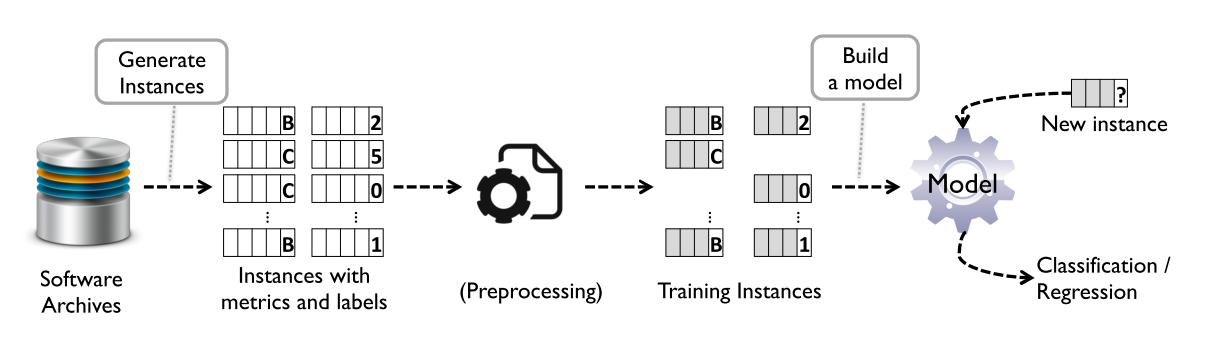
\includegraphics[width=1.0\textwidth]{img/prediction-process.PNG}
	 \caption{فرآیند پیش‌بینی خطا \cite{nam2014survey}}
	\label{fig:prediction-process}
\end{figure}
\subsection{اندازه‌های ارزیابی}
\label{subsec:eval}
معیارهای ارزیابی را می‌توان به دسته‌ی کلی  معیارهای دسته‌بندی و رگرسیون تقسیم کرد.  معیارهای دسته بندی را می‌توان با استفاده از \واژه{ماتریس درهم‌ریختگی} محاسبه نمود. در ماتریس درهم ریختگی پیش‌بینی خطا، عناصر  به صورت زیر تعریف می‌شوند.  همچنین نحوه‌ی محاسبه‌ی معیارها در جدول \ref{tab:eval-metircs} آمده است. 
\begin{itemize}
	\setlength\itemsep{.01em}
\item 
مثبت واقعی: 
تعداد داده‌های حاوی خطا که به درستی تشخیص داده شدند
\item
مثبت اشتباه:
تعداد داده‌های سالم که به عنوان خطادار پیش‌بینی شدند
\item 
منفی اشتباه:
تعداد داده‌های سالم که به درستی تشخیص داده شدند
\item 
منفی واقعی:
تعداد داده‌های حاوی خطا که به عنوان داده‌ی سالم پیش‌بینی شدند

\end{itemize}


\begin{table}[H] 
		\renewcommand*{\arraystretch}{1.5}	
	\centering \caption{فرمول‌های محاسبه‌ی معیارهای ارزیابی}
	\label{tab:eval-metircs}
	\newcolumntype{C}{>{\centering\arraybackslash} m } 

	\begin{tabular}{|C{1.5cm} |C{2cm}|C{4.5cm}|C{6cm} |}
 
	\hline
	\hline
	نام معیار & نام لاتین & نحوه‌ی محاسبه & توضیح
		\\
	\hline
	\hline
	نرخ مثبت اشتباه &
	\lr{False Positive Rate (PF)}  &
	$ \displaystyle \frac{FP}{TN+FP} $ &
	نسبت تعداد داده‌هایی که به اشتباه خطادار پیش‌بینی شده‌اند به تعداد کل داده‌های بدون خطا
	\\
	\hline
	صحت & 
		\lr{Accuracy} & $ \displaystyle \frac{TP+TN}{TP+FP+TN+FN}$ &
	نسبت	تعداد پیش‌بینی‌های درست به تعداد کل پیش‌بینی‌ها
		
	\\
	\hline
	دقت &
	\lr{Precision} & $\displaystyle \frac{TP}{TP+FP}$ &
نسبت تعداد داده‌هایی که به درستی خطادار پیش‌بینی شده‌اند به تعداد کل داده‌هایی که خطادار پیش‌بینی شده‌اند
	\\
	\hline
	بازخوانی & 
	\lr{Recall (PD)} & $\displaystyle \frac{TP}{TP+FN}$ &
	نسبت تعداد داده‌هایی که به درستی خطادار پیش‌بینی شده‌اند به تعداد کل داده‌های خطادار
	\\
	\hline
	معیار اف &
	\lr{F-Measure} & $ \displaystyle \frac{2 \times Precision \times Recall}{Precision + Recall}$ &
	از آنجا که در بین معیارهای دقت و بازخوانی مصالحه وجود دارد معیار اف ترکیبی از آن دو را در نظر می‌گیرد
	\\
	\hline
	\end{tabular}
\end{table}

در ادامه به بررسی و تحلیل هر یک از این معیارها پرداخته می‌شود. 
\begin{itemize}
	\item 
	نرخ مثبت اشتباه: نام دیگر این معیار \واژه{احتمال اخطار اشتباه} می‌باشد. هر چقد که یک مدل پیش‌بینی به اشتباه داده‌ها را خطادار پیش‌بینی کند مقدار این معیار بیشتر می‌شود تا جایی که اگر مدل پیش‌بینی هیچ داده‌ای را بدون خطا پیش‌بینی نکند مقدار آن یک می‌شود و اگر داده‌ای را به اشتباه حاوی خطا معرفی نکند مقدار معیار صفر می‌شود. 
\item 
صحت: این معیار نسبت تعداد پیش‌بینی‌های مثبت واقعی و منفی واقعی را به تعداد کل پیش‌بینی‌ها می‌سنجد. اگرچه میزان پیش‌بینی‌های درست در این معیار سنجیده می‌شود. اما معیار صحت نمی‌تواند در مواردی که مجموعه‌داده‌ها نا‌متوازن است معیار مناسبی باشد. به عنوان مثال اگر در یک مجموعه‌داده ۱۰ درصد از داده‌ها حاوی خطا باشد آنگاه  در مدلی که همواره داده‌ها را بدون خطا پیش‌بینی می‌کند این معیار مقدار ۹۰ درصد می‌گیرد در صورتی که این مدل مناسب نیست. 
\item
دقت: نام دیگر این معیار \واژه{ارزش پیش‌بینی مثبت} می‌باشد. این معیار نشان دهنده‌ی آن است که به چه میزان داده‌های پیش‌بینی شده به عنوان خطادار درست پیش‌بینی شده است.  در صورتی که همه‌ی داده‌هایی که خطادار معرفی شده‌اند در واقعیت نیز حاوی خطا باشد این معیار مقدار یک می‌یابد. 
\item 
بازخوانی: این معیار مشخص می‌کند که چه مقدار از داده‌هایی که باید به عنوان خطادار معرفی می‌شدند در واقع توسط مدل خطادار پیش‌بینی شده‌اند.  زمانی که این معیار برابر یک می‌باشد بدان معنی است که تمام داده‌‌های حاوی خطا شناسایی شده‌اند. البته ممکن است برخی داده‌های بدون خطا نیز خطا دار پیش‌بینی شوند و همچنان معیار بازخوانی مقدار یک را داشته باشد. همانطور که در جدول \ref{tab:eval-metircs} مشخص شده ‌است بین دقت و بازخوانی یک \واژه{مصالحه} وجود دارد. این بدان معنی است که اغلب می‌توان یکی را به هزینه‌ی کاهش دیگری افزایش داد. 
\item
معیار اف: از آنجا که در محاسبه‌ی این معیار از ترکیب دقت و بازخوانی استفاده می‌شود از معایب بررسی جداگانه این دو معیار کاسته می‌شود. در برخی موارد اهمیت دقت و بازخوانی یکسان نیست که باید از نوع دیگری از معیار اف استفاده که دارای وزن‌دهی می‌باشد. 
\end{itemize}





دو اندازه دیگر نیز که در پژوهش‌ها کاربرد دارند عبارتند از \واژه{مساحت زیر منحنی} و \واژه{مساحت زیر منحنی هزینه-اثربخشی}. در محاسبه‌ی مساحت زیر منحنی از  نمودار \واژه{مشخصه‌ی عملکرد دریافت‌کننده} استفاده می‌شود . در این نمودار محورهای عمودی و افقی را به ترتیب بازخوانی و  نرخ مثبت کاذب تشکیل می‌دهد.  با تغییر \واژه{آستانه‌ی تصمیم} برای یک مدل می‌توان میزان بازخوانی و  نرخ مثبت کاذب را تغییر داده و بدین ترتیب منحنی را رسم نمود.  منظور از آستانه‌ی تصمیم  مرزی است  که یک مدل یک داده را حاوی خطا پیش‌بینی می‌کند یا سالم. به عنوان مثال زمانی که آستانه برابر ۳۰ درصد است در صورتی که یک داده به احتمال ۳۱ درصد حاوی خطا باشد آن داده به عنوان خطادار پیش‌بینی می‌شود. \\

یک مدل بی‌نقص دارای مساحت زیر نمودار 1 است.  مدل بی‌نقص مدلی است که تمام پیش‌بینی‌ها را به درستی انجام می‌دهد. این مدل  در برخورد با داده‌ی حاوی خطا ۱۰۰ درصد احتمال می‌دهد که حاوی خطا است  و برای داده‌ی سالم صفر درصد احتمال می‌دهد حاوی خطا است. اگر بخواهیم منحنی را برای مدل بی‌نقص رسم کنیم در ابتدا آستانه  برابر یک  در نظر گرفته می‌شود. در نتیجه همه‌ی داده‌ها بدون خطا دسته‌بندی می‌شوند. در این حالت نرخ مثبت اشتباه برابر صفر است زیرا هیچ داده‌ای به اشتباه خطادار معرفی نشده. بازخوانی نیز صفر است چون هیچ داده‌ای به درستی خطادار پیش‌بینی نشده. پس منحنی از نقطه‌ی صفر و صفر آغاز می‌شود. زمانی که آستانه اندکی از یک کمتر شود مدل همه‌ی پیش‌بینی‌ها را به درستی انجام می‌دهد و نرخ مثبت اشتباه برابر صفر و بازخوانی برابر یک خواهد بود. در نتیجه نقطه‌ی دیگر  بر روی منحنی در بالا سمت چپ منحنی است. با کمتر کردن آستانه تغییری در محل نقطه ایجاد نمی‌شود تا زمانی که آستانه به صفر برسد. در این حالت همه‌ی داده‌ها خطادار پیش‌بینی می‌شوند. نرخ مثبت اشتباه برابر یک خواهد شد چون هیچ داده‌ای سالم پیش‌بینی نشده است و بازخوانی برابر یک خواهد بود چون همه‌ی داده‌هایی که باید خطادار پیش‌بینی می‌شدند خطا‌دار پیش‌بینی شده‌اند. در نتیجه نقطه‌ی دیگر در بالا راست نمودار خواهد بود و مساحت زیر نمودار برابر یک خواهد بود. \\

برای یک مدل تصادفی  منحنی از مبدا به نقطه‌ی (1\lr{,}1) رسم خواهد شد. یک نمونه از منحنی مشخصه‌ی عملکرد دریافت‌کننده در شکل \ref{fig:ROC} آمده است. \\

\begin{figure}
	\centering
	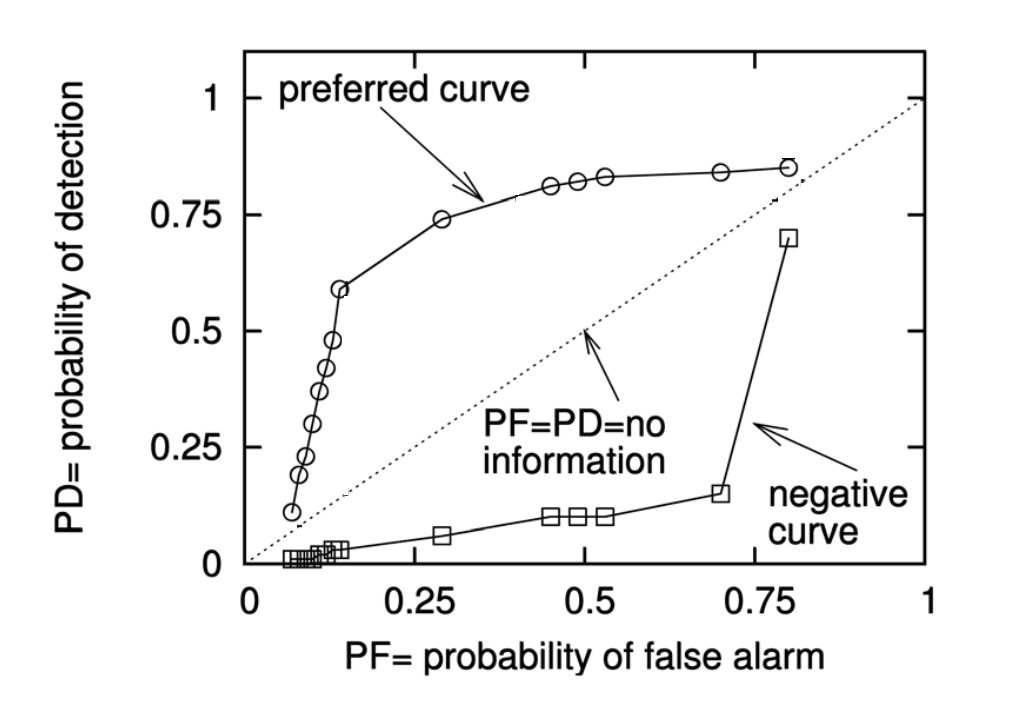
\includegraphics[width=.60\textwidth]{img/ROC.PNG}
	\caption{ نمونه‌ای از نمودار \lr{ROC} \cite{menzies2007data}}
	\label{fig:ROC}
\end{figure}

 مساحت زیر منحنی هزینه-اثربخشی معیاری است که تعداد خطوطی از برنامه که  توسط تیم تضمین کیفیت و یا توسعه‌دهندگان نیاز است بررسی و آزمون شود را در نظر می‌گیرد. منظور از بررسی بازبینی کد جهت یافتن خطا بدون استفاده از روش‌های مرسوم آزمون نرم‌افزار می‌باشد. ایده‌ی  موثر بودن از نظر هزینه
برای مدل‌های ‌‌ پیش‌بینی خطا برای اولین بار توسط آریشلم و همکاران \cite{arisholm2007data} ارائه گردید. موثر بودن از نظر هزینه به این معنا است که چه تعداد خطا با بررسی و یا آزمون  \lr{n}  درصد اول خطوط می‌توان یافت. به عبارت دیگر اگر یک مدل پیش‌بینی خطا بتواند تعداد خطای بیشتری را با بررسی و تلاش در آزمون کمتر، نسبت به باقی مدل‌ها بیابد می‌توان گفت که تاثیر آن از نظر هزینه بیشتر است. دو منحنی در  قسمت راست شکل \ref{fig:AUCEC} برای دو مدل پیش‌بینی مختلف آمده است. هر دو مدل دارای سطح زیر نمودار یکسانی هستند اما زمانی که ۲۰ درصد اول محور افقی در نظر گرفته می‌شود مدل 
\lr{P$_2$}
  کارایی بهتری دارد. نمودار سمت چپ مدل‌های تصادفی، عملی\LTRfootnote {Practical} و بهینه را نشان می‌دهد.

\begin{figure}[H]
	\centering
	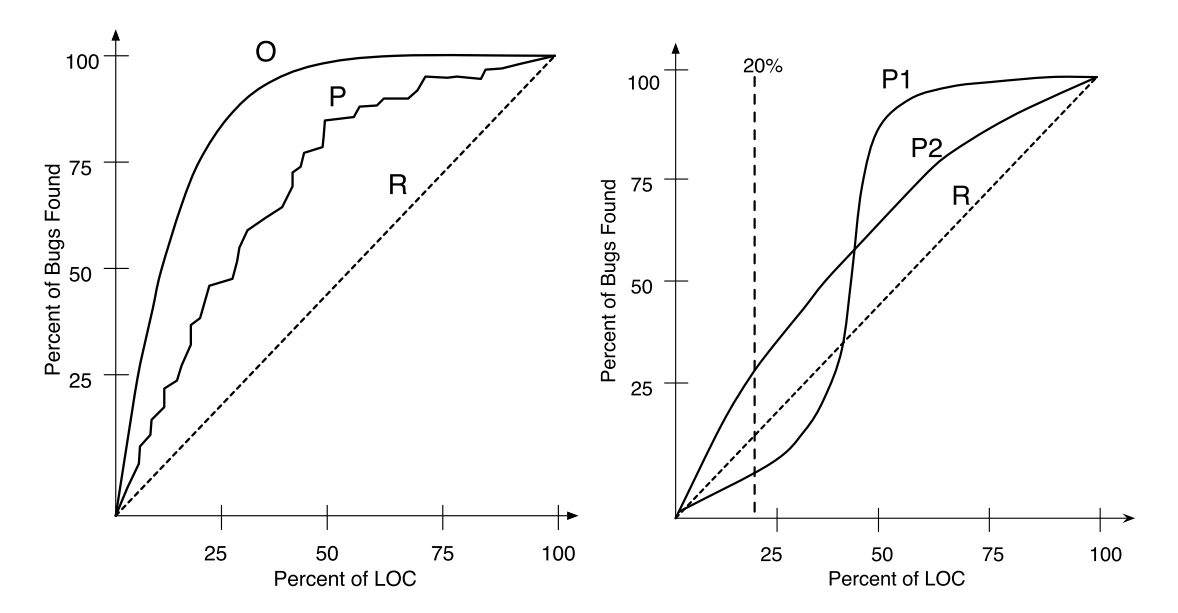
\includegraphics[width=.7\textwidth]{img/AUCEC.PNG}
	\begin{tabular}{c c c}
		\lr{O = optimal} & \lr{P = practical} &  \lr{R = random}\\
	 
	\end{tabular}
	\caption{ نمودار موثر بودن از نظر هزینه \cite{rahman2011bugcache}}
	\label{fig:AUCEC}
\end{figure}

معیارهایی که برای ارزیابی نتایج حاصل از روش رگرسیون به کار گرفته می‌شوند بر اساس همبستگی\LTRfootnote{Correlation} میان تعداد خطاهای پیش‌بینی شده و خطاهای واقعی محاسبه می‌شوند. نماینده‌ی این معیارها را می‌توان همبستگی اسپیرمن، پیرسون و $ R^2$ دانست \cite{nam2014survey}. 
\subsection{معیارهای پیش‌بینی خطا}
\label{subsec:metrics}
معیارهای پیش‌بینی خطا نقش مهمی را در ساخت مدل پیش‌بینی ایفا می‌کنند. اکثریت معیارهای پیش‌بینی خطا را می‌توان به دو دسته‌ی  کلی تقسیم کرد: معیارهای کد و معیارهای فرآیند. معیارهای کد می‌توانند به طور مستقیم از کدهای منبع موجود جمع آوری شوند در حالی که معیارهای فرآیند  از اطلاعات تاریخی که در مخازن نرم‌افزاری مختلف آرشیو شده‌اند استخراج می‌گردند. نمونه‌ای از این مخازن نرم‌افزاری سیستم‌های کنترل نسخه و سیستم‌های ردگیری خطا است. معیار‌های فرآیند از نظر هزینه موثر تر از سایر معیارها هستند\cite{arisholm2010systematic}. در برخی از مقالات نیز معیارهای  پیش‌بینی خطا به سه دسته‌ی: معیارهای کد منبع سنتی، معیارهای شئ‌گرایی و معیارهای فرآیند تقسیم شده‌اند\cite{radjenovic2013software}.\\\\
\textbf{معیارهای کد} \\

معیارهای کد تحت عنوان \واژه{معیارهای محصول} نیز شناخته می‌شوند و میزان پیچیدگی کد را می‌سنجند. \واژه{فرض زمینه‌ای} آنها این است که هرچه کد پیچیده‌تر باشد خطا‌خیز‌تر است. برای اندازه‌گیری پیچیدگی کد پژوهش‌گران معیار‌های مختلفی را ارائه داده‌اند که در ادامه مهم‌ترین آنها معرفی خواهند شد. 

این معیارها با استفاده از اندازه‌های مطرح شده در جدول \ref{tab:measure}  استخراج شده‌اند. 

\begin{table}[H] 
	\renewcommand*{\arraystretch}{1.5}	
	\centering \caption{اندازه‌های به کارگرفته شده  در معیارهای کد }
	\label{tab:measure}
	\newcolumntype{C}{>{\centering\arraybackslash} m } 
	\begin{tabular}{|C{2cm}|C{2cm}|C{1.5cm}|C{8cm}|}
		
		\hline
		\hline
		نام & نام لاتین & علامت اختصاری & توضیح \\
		\hline
		\hline
		تعداد خطوط کد & 		\lr{Line of Code}  & LOC		& این اندازه را می‌توان به اندازه‌های جزیی‌تر مانند تعداد خطوط توضیح، قابل اجرا، خالی از نوشته تقسیم کرد \\
		\hline
		تعداد عملگرها & \lr{Number of Operators} & 
		\lr{$N_1$}
		& تعداد عملگرهای موجود مانند + ، - ، \& \\
		\hline
		 
		تعداد عملوندها&  \lr{Number of Operands} & 
		\lr{$N_2$}
		& تعداد عملوندهای استفاده شده در کنار عملگرها\\
		\hline
			تعداد عملگرهای متمایز & \lr{Number of Unique Operators} & 
		\lr{$\eta_1$}
		& ---\\
		\hline
		
		تعداد عملوندهای متمایز &  \lr{Number of Unique Operands} & 
		\lr{$\eta_2$}
		& ---\\
		\hline
		
تعداد یال‌ها &   \lr{Number of Edges} &  E &  تعداد یال‌های گراف جریان کنترلی\\
		\hline
		تعداد گره‌ها &    \lr{Number of Nodes} & N & تعداد گره‌ها در گراف جریان کنترلی \\
		\hline
		
		تعداد قطعات متصل &    \lr{Number of Connected Component} & P  & تعداد قطعات متصل به هم در گراف جریان کنترلی
		\\
		\hline
		
	\end{tabular}
\end{table}


\begin{itemize}
	\item \textbf{معیار بزرگی: }
معیارهای \واژه{بزرگی} اندازه‌ی کلی و حجم کد را می‌سنجند. یکی از اندازه‌های برجسته که در محاسبه‌ی این معیارها و گاها خود به تنهایی به کار می‌رود "تعداد خطوط" می‌باشد. اولین بار \نام{آکیاما}{Akiyama}
 \cite{akiyama1971example}  
رابطه‌ی میان خطا و تعداد خطوط را مطرح کرد. \نام{هالستد}{Halstead}
 \cite{halstead1977elements} 
 چندین معیار بزرگی بر اساس  تعداد عملگرها و عملوند‌ها ارائه داده است و در مقاله‌ی \cite{pawade2016exploring} مورد بازنگری قرار گرفته است. معیارهایی که توسط هالستد مطرح شده‌اند در زیر آمده آمده‌اند که با استفاده از اندازه‌های جدول \ref{tab:measure} محاسبه می‌شوند. 
 \begin{latin}
 \baselineskip=1.1cm
Lenght: $N = N_1 + N_2$ \\
Volume: $V = N \times log_2 (\eta_1 + \eta_2)$\\
Difficulty: $D = \eta_1/2 \times N_2/\eta_2$ \\
Effort: $E = D \times V$ \\
Program Time: $T = E/18$ \\
 \end{latin}
 
 
\item \textbf{معیار پیچیدگی حلقوی: }
\نام{مک‌کیب}{McCabe} معیارهای \واژه{پیچیدگی حلقوی}
را پیشنهاد داد که این معیار با استفاده از تعداد گره‌ها، یالها و قطعات متصل در گراف  \واژه{جریان کنترلی} کد منبع محاسبه می‌گردد\cite{mccabe1976complexity}. این معیارها نشان می‌دهند که راه‌های کنترلی به چه میزان پیچیده هستند. باوجود اینکه جز اولین معیارها بوده است همچنان در پیش‌بینی خطا کاربرد دارد \cite{malhotra2014comparative}. این معیار با استفاده با استفاده از فرمول زیر محاسبه می‌شود. 
\begin{latin}
$V(G) = E - N + 2P $
\end{latin}


\item \textbf{معیار مربوط به شئ‌گرایی: }
با ظهور زبان‌های شئ‌گرایی و محبوبیت آنها معیارهای کد  برای این زبان‌ها ارائه شد تا فرآیند توسعه بهبود یابد. نماینده‌ی این معیارها CK می‌باشد که توسط \نام{چدامبر و کمرر}{Chidamber and Kemerer  \lr{(CK)} }
 ارائه شده است\cite{chidamber1994metrics}. این معیارها  که در جدول  \ref{tab:ck-metrics} لیست آنها قرار داده شده، با توجه به خصیصه‌های زبان‌های شئ‌گرا مانند وراثت، \واژه{زوجیت}، \واژه{همبستگی} طراحی شده‌اند. بجز معیارهای  \چر{CK}، معیارهای شئ‌گرایی دیگری نیز بر اساس حجم و کمیت کد منبع پیشنهاد داده شده‌اند. مشابه معیارهای \موکد{اندازه}، معیارهای شئ‌گرایی تعداد نمونه‌های یک کلاس، توابع را می‌شمارند. \\
 \begin{table}[H] 
 	\renewcommand*{\arraystretch}{1.5}	
 	\centering \caption{معیارهای CK }
 	\label{tab:ck-metrics}
 	\newcolumntype{C}{>{\centering\arraybackslash} m } 
 	\begin{tabular}{|C{2cm}|C{3cm}|C{8cm}|}
 		
 		\hline
 		\hline
 		نام & توضیح & نحوه‌ی محاسبه \\
 		\hline
 		\hline
 		WMC &
 		تعداد توابع وزن‌دهی شده & وزن دهی بر اساس پیچیدگی هر تابع انجام می‌شود \\
 		\hline
DIT & 
عمق درخت وراثت & حداکثر طول مسیر در در از نوادگان یک کلاس تا خود کلاس\\
\hline
NOC &
تعداد فرزندان & تعداد نوادگان مستقیم کلاس\\
\hline
CBO & 
زوجیت میان اشیاء کلاس‌ها & تعداد کلاس‌هایی که کلاس مورد نظر با آن زوج شده‌است. دو کلاس با هم زوجیت دارند اگر یکی از توابع و یا متغر‌های دیگری استفاده کرده باشد. \\
\hline
RFC &
پاسخ برای یک کلاس & تعداد توابعی که با فراخوانی یک تابع از کلاس احتمال فراخوانی دارند. برابر است با تعداد کل توابع کلاس و توابعی از سایر کلاس‌ها که در آنها فراخوانی می‌شوند. \\
\hline
LCOM & 
کمبود همبستگی میان توابع & تعداد جفت توابعی که متغیر مشترک ندارند منهای جفت توابعی که متغیر مشترک دارند. \\
 		
 		\hline

\end{tabular}
\end{table}

\end{itemize}
\textbf{معیارهای فرآیند} \\

در ادامه  تعدادی از معیارهای فرآیند بررسی می‌شوند که در این دسته شاخص محسوب می‌شوند. در جدول \ref{tab:process-measure} اندازه‌هایی که در محاسبه‌ی معیارهای فرآیند به کار گرفته شده‌اند آمده است.
\begin{table}[H] 
	\renewcommand*{\arraystretch}{1.5}	
	\centering \caption{اندازه‌های به کارگرفته شده  در معیارهای فرآیند }
	\label{tab:process-measure}
	\newcolumntype{C}{>{\centering\arraybackslash} m } 
	\begin{tabular}{|C{2cm}|C{2cm}|C{2.25cm}|C{7.25cm}|}
		
		\hline
		\hline
		نام & نام لاتین & علامت اختصاری & توضیح \\
		\hline
		\hline
		تعداد خطوط تبدیلی &  Churned LOC & --- & تعداد خطوط اضافه شده به علاوه‌ی خطوط تغییر داده شده در دو نسخه‌ی متفاوت از برنامه \\
		\hline
		تعداد فایل‌های تبدیلی &
		\lr{Files Churned} & --- &
		تعداد فایل‌های تغییر یافته در یک قطعه \\
		\hline
		تعداد فایل‌ها &
		\lr{Files Count} & --- &
		تعداد فایل‌های موجود در یک قطعه\\
		\hline
		تجدیدنظر‌ها &
		\lr{Revisions} & --- &
		تعداد تجدید نظرهایی (اصلاح‌ها) که در فایل انجام شده است\\
		\hline 
		بازآرایی & 
		Refactoring & --- & 
		تعداد دفعاتی که یک فایل بازآرایی شده است. در واقع تعداد ثبت‌هایی شمرده می‌شود که در توضیح آنها کلمه‌ی refactor وجود داشته باشد.\\
		\hline
		تعداد ایمیل‌ها &
		\lr{Number of Mails} & POP\_NOM &
		 تعداد ایمیل‌هایی که در آنها نام کلاس مورد نظر آورده شده است.\\
		 \hline
		 تعداد نخ‌ها &
		 \lr{Number of Threads} & POP\_NOT &
		 تعداد نخ‌هایی که درباره‌ی یک کلاس صحبت می‌کنند \\
		 \hline
		 تعداد نویسندگان &
		 \lr{ Number of Authors}& POP\_NOA &
		 تعداد نویسندگانی که درباره‌ی کلاس مورد نظر صحبت می‌کنند. \\
		 \hline
	\end{tabular}
\end{table}

\begin{itemize}
\item \textbf{تغییر تبدیلی نسبی کد: }
\نام{ناگاپان و بال}{Nagappan and Ball} هشت معیار تغییر \واژه[تبدیلی]{تبدیل} نسبی کد را ارائه داده‌اند\cite{nagappan2005use}. دو مثال از این معیارها در زیر آمده است.  در معیار $M_1 $ تعداد تجمعی خطوط اضافه و حذف شده بین دو نسخه از برنامه را می‌شمارد و بر تعداد خطوط برنامه تقسیم می‌کند. معیار دیگر تعداد فایل‌های تغییر یافته از یک قطعه برنامه را بر تعداد  کل فایل‌ها تقسیم می‌کند. 
\begin{latin}
\baselineskip=1.1cm
$M_1 = Churned LOC / Total LOC$\\
$M_2 = Files Churned / Files Count$
\end{latin}

\item \textbf{معیارهای تغییر: }
این معیارها  گستره‌ی تغییرات در تاریخچه‌ی ذخیره شده در سامانه‌ی کنترل نسخه را اندازه می‌گیرند. به عنوان مثال تعداد رفع خطاها، تعداد \واژه{بازآرایی کد} و یا تعداد نویسندگان یک فایل را می‌شمارند. \نام{موزر}{Moser} و همکاران 18 معیار تغییر را از مخازن \نام{اکلیپس}{Eclipse} استخراج کردند و یک تحلیل مقایسه‌ای میان معیارهای کد و معیارهای تغییر انجام دادند. آنها به این نتیجه رسیدند که معیارهای تغییر پیش‌بینی کننده‌ی بهتری از معیارهای کد هستند.  به عنوان نمونه دو مورد از ۱۸ معیار مطرح شده برابر اندازه‌های \موکد{تجدیدنظر‌ها} و \موکد{بازآرایی} است.

\item \textbf{معیارهای شهرت: }
 \نام{بکچلی}{Bacchelli} و همکاران معیارهای \واژه{شهرت} را بر اساس تحلیل ایمیل‌های آرشیو شده‌ی نویسندگان ارائه داده‌اند. ایده‌ی اصلی این معیارها این است که یک قطعه‌ی  نرم‌افزاری که در ایمیل‌ها درباره‌ی آن بیشتر صحبت شده است خطاخیزتر می‌باشد\cite{bacchelli2010popular}.  بکچلی پنج معیار شهرت معرفی کرده است.  به عنوان نمونه سه مورد از آنها  برابر است با اندازه‌های \موکد{تعداد ایمیل‌ها، تعداد نخ‌ها و تعداد نویسندگان}. \\
\end{itemize}


\نام{راجنویک}{Radjenovic} و همکاران در پژوهش خود به \واژه{بررسی قاعده‌مند} معیارهای پیش‌بینی خطا در مطالعات پیشین پرداخته‌اند.  طبق این پژوهش در 49\lr{\%} مطالعات از معیارهای شئ‌گرایی، در 27\lr{\%} معیارهای سنتی کد و در 26 \lr{\%} از معیارهای فرآیند استفاده شده است. با توجه به مطالعات بررسی شده دقت پیش‌بینی خطا  با انتخاب معیارهای مختلف، تفاوت قابل توجهی  پیدا می‌کند. معیارهای شئ‌گرایی و فرآیند موفق‌تر از معیارهای سنتی هستند. معیارهای سنتی  پیچیدگی کد، قویا با معیارهای اندازه مانند تعداد خطوط کد همبستگی دارند و این دو توانایی پیش‌بینی خطا دارند اما جز بهترین معیارها نیستند. معیارهای شئ‌گرایی بهتر از اندازه و پیچیدگی عمل می‌کنند و با این که با معیارهای اندازه همبستگی دارند اما ویژگی‌های بیشتری علاوه بر اندازه را دارند. معیارهای ایستای کد همانند اندازه، پیچیدگی و شئ‌گرایی به منظور بررسی یک نسخه از برنامه مفید هستند اما با هر \واژه{تکرار} در فرآیند توسعه‌ی نرم‌افزار دقت پیش‌بینی آنها کاسته می‌شوند و معیارهای فرآیند در چنین شرایطی بهتر عمل می‌کنند.  با این وجود  که  معیارهای فرآیند‌  دارای توانمندی بالقوه‌ای  هستند، اما در تعداد کمتری از پژوهش‌ها مورد استفاده قرار گرفته‌اند\cite{radjenovic2013software}. \\
 
\نام{آسترند}{Ostrand} و همکاران به بررسی این موضوع پرداخته‌اند که آیا اطلاعاتی درباره‌ی اینکه کدام توسعه‌دهنده یک فایل را اصلاح می‌کند قادر است که پیش‌بینی خطا را بهبود بخشد. در پژوهش قبلی آنها\cite{weyuker2008too} مشخص شده بود که تعداد کلی   افراد توسعه‌دهنده در یک فایل می‌تواند در پیش‌بینی خطا تاثیر متوسطی داشته باشد. در  مقاله‌ی \cite{ostrand2010programmer}  تعدادی از متغیرهای کد منبع و فرآیند به همراه معیار مرتبط به توسعه‌دهنده در نظر گرفته شده است.  در این پژوهش مشخص شد  که تعداد خطاهایی که یک توسعه‌دهنده تولید می‌کند ثابت است و با سایر توسعه دهندگان فرق دارد. این تفاوت با  حجم کدی که یک توسعه‌دهنده اصلاح می‌کند مرتبط است و در نتیجه در نظر گرفتن یک نویسنده خاص نمی‌تواند به بهبود پیش‌بینی خطا کمک کند\cite{ostrand2010programmer}. \\

\نام{رحمان و دوانبو}{Rahman and Devanbu} از جنبه‌های مختلف معیارهای فرآیند  را با سایر معیارها مقایسه کرده‌اند\cite{rahman2013and}. نتایج نشان می‌دهد  زمانی که مدل پیش‌بینی بر روی یک نسخه آموزش می‌بیند و در نسخه‌ی بعدی آزمون می‌شود معیارهای کد، مساحت زیر منحنی  قابل قبولی دارند اما مساحت آنها کمتر از معیارهای فرآیند است  و از نظر معیار مساحت زیر نمودار هزینه-اثربخشی ۲۰ درصد 
بهتر از یک مدل تصادفی عمل نمی‌کنند و  به آن معنی است که این معیارها از نظر هزینه چندان  موثر نیستند. همچنین معیارهای کد ایستاتر هستند، ‌یعنی با تغییرات پروژه و تغییر در توزیع خطاها همچنان معیارها بدون تغییر باقی می‌مانند. معیار ایستا تمایل دارد یک فایل را در \واژه[انتشارهای]{انتشار} متوالی همچنان حاوی خطا معرفی کند. معیارهای ایستا به مدل‌های راکد منجر می‌شوند که این مدل‌ها به سمت فایل‌های بزرگ با تراکم خطای کمتر \واژه{جهت‌گیری} دارند. به عنوان مثال حالتی را در نظر بگیرید که در یک پروژه فایل‌های بزرگ و پیچیده‌ای وجود دارد که پس از چندین انتشار خطاهای آنها برطرف می‌شود اما مدل‌هایی که بر اساس معیارهای کد ساخته شده‌اند همچنان این فایل‌ها را به عنوان خطا‌خیز معرفی می‌کنند. از طرف دیگر حالتی را در نظر بگیرید که یک فایل با اندازه و پیچیدگی کم به تازگی به وجود آمده و یا تغییرات فراوان یافته است. مدل‌های مبتنی بر کد به این فایل‌ها توجه چندانی نخواهند کرد در حالیکه که این فایل‌ها مستعد وجود خطا هستند. بدین ترتیب معیارهای فرآیند بهتر از معیارهای کد عمل می‌کنند. \\
معیارهای استفاده شده در این مقاله در جدول \ref{tab:process-measure} آورده شده‌اند. در ادامه هر یک از معیارها به طور مشروح توضیح داده می‌شوند. 
 
 \begin{table}[H] 
 	\renewcommand*{\arraystretch}{1.5}	
 	\centering \caption{معیارهای فرآیند 
 		\cite{rahman2013and}}
 	\label{tab:process-metircs}
 	\newcolumntype{C}{>{\centering\arraybackslash} m } 
 	\newcounter{magicrownumbers}
 	\def\rownumber{}
 	\setcounter{magicrownumbers}{0}
 	\begin{tabular}{|@{\makebox[3em][c]{\rownumber\space}} |c|c|}
 		
 		\hline
 		\hline
 		نام معیار  & توضیح
 		\gdef\rownumber{\stepcounter{magicrownumbers}\arabic{magicrownumbers}} 
 		\\
 		
 		\hline
 		\hline
 		\lr{COMM } & تعداد ثبت در سیستم کنترل نسخه
 		\\
 		\hline
 		\lr{ADEV} & تعداد توسعه‌دهندگان فعال
 		\\ 
 		\hline
 		\lr{DDEV} & تعداد توسعه‌دهندگان متمایز
 		\\ 
 		\hline
 		\lr{ADD} &  مقدار نرمال‌سازی شده‌ی تعداد خطوط اضافه شده
 		\\ 
 		\hline
 		\lr{DEL}  & مقدار نرمال‌سازی شده‌ی تعداد خطوط حذف شده
 		\\ 
 		\hline
 		\lr{OWN} &  درصد خطوطی که مالک پرونده مشارکت کرده
 		\\ 
 		\hline
 		\lr{MINOR} & تعداد مشارکت‌کنندگان جزئی
 		\\ 
 		\hline
 		\lr{NCOMM} & تعداد ثبت‌های همسایگان
 		\\ 
 		\hline
 		\lr{NADEV} & تعداد توسعه‌دهندگان فعال همسایگان
 		\\ 
 		\hline
 		\lr{NDDEV} & تعداد توسعه‌دهندگان متمایز همسایگان
 		\\ 
 		\hline
 		\lr{OEXP} & تجربه‌ی مالک پرونده
 		\\ 
 		\hline
 		\lr{AEXP} & تجربه‌ی تمام مشارکت‌کنندگان
 		\\ 
 		\hline
 		
 	\end{tabular}
 \end{table}

\begin{enumerate}
	\item
	\textbf{تعداد ثبت در سیستم کنترل نسخه:}
	تعداد ثبت‌هایی که در آن پرونده‌ی ‌مورد نظر در طول انتشار قبلی تاکنون تغییر کرده است. برای محاسبه ی آن لازم است که تمام ثبت‌های پروژه بین ثبت کنونی و \واژه{انتشار} قبلی بررسی شود و ثبت‌هایی که در آن این پرونده تغییر کرده‌اند شمرده شوند.
	\item
	\textbf{تعداد توسعه‌دهندگان 
		فعال:}
	تعداد توسعه‌دهندگانی که در طول انتشار قبلی تا کنون (زمان ثبت) پرونده را تغییر داده‌اند. لازم است ثبت‌های موجود در باز‌ه‌ی زمانی خواسته شده بررسی شود و آنها که پرونده مورد نظر را تغییر داده‌اند انتخاب شوند. نام کسانی که ثبت را انجام داده‌اند بازیابی شود و تعداد نام‌های متمایز شمرده شود. 
	\item
	\textbf{تعداد توسعه‌دهندگان	متمایز:}
	مشابه معیار قبلی با این تفاوت که در طول انتشار محاسبه نمی‌شود. بلکه از ابتدای پروژه تا زمان ثبت در نظر گرفته می‌شود. 
	\item
	\textbf{مقدار نرمال‌سازی شده‌ی تعداد خطوط اضافه شده:}
	این معیار تعداد خطوط اضافه شده در یک پرونده را در طول انتشار قبلی می‌شمارد. سپس جهت نرمال سازی آنرا بر تعداد کل خطوط اضافه شده در پروژه در طول انتشار قبلی تقسیم می‌کند. برای بدست آوردن تعداد خطوط اضافه شده در یک پرونده هر ثبت نسبت به ثبت قبلی مقایسه می‌شود و تعداد خطوط اضافه شده جمع زده می‌شود.
	\item
	\textbf{مقدار نرمال‌سازی شده‌ی تعداد خطوط حذف شده:}
	مشابه معیار قبلی می‌باشد. 
	\item
	\textbf{تعداد خطوطی که مالک پرونده مشارکت کرده:}
	درصد خطوطی  از پرونده، در  ثبت مورد نظر  که به مالک پرونده تعلق دارد. مالک پرونده کسی است که در آن لحظه از زمان بیشترین تعداد خطوط موجود در پرونده به او تعلق دارد. ابتدا نویسنده‌ی هر خط مشخص می‌شود سپس برای هر نویسنده تعداد خطوطی که به وی تعلق دارد شمرده می‌شود. تعداد خطوط مالک پرونده بر تعداد خطوط پرونده تقسیم می‌گردد.
	\item
	\textbf{تعداد مشارکت‌کنندگان جزئی:}
	مشارکت‌کننده‌ی جزئی کسی است که کمتر از ۵٪ خطوط موجود در پرونده به او تعلق داشته باشد. بدین منظور نویسنده‌ی هر خط مشخص می‌شود. تعداد خطوط هر نویسنده شمرده می‌شود و بر تعداد خطوط پرونده تقسیم می‌شود. سپس تعداد نویسندگانی که کمتر از ۵٪ مشارکت داشته‌اند شمرده می‌شود. 
	\item
	\textbf{تعداد ثبت‌های همسایگان:}
	میانگین وزن دهی شده تعداد ثبت‌های همسایگان پرونده از انتشار قبلی تا کنون را اندازه‌گیری می‌کند. همسایگان یک پرونده در یک ثبت، پرونده‌هایی هستند که در آن نسخه از برنامه تغییر کرده‌اند. در‌واقع در هر ثبت از برنامه تعدادی پرونده نسبت به ثبت قبلی تغییر کرده‌اند که این پرونده‌ها همسایه‌ی یکدیگر محسوب می شوند. نحوه‌ی وزن دهی نیز به این صورت است که هرچقدر یک پرونده تعداد دفعات بیشتری را در طول انتشار با پرونده مورد نظر همسایه شده باشد وزن بیشتری می‌یابد. برای محاسبه ابتدا همسایگان پرونده در ثبت  و تعداد دفعاتی که  در طول انتشار همسایه شده‌اند مشخص می‌شوند. سپس برای هر پرونده‌ی همسایه، معیار تعداد ثبت در سیستم کنترل نسخه محاسبه می‌شود. هر معیار در تعداد دفعاتی همسایگی ضرب می‌شود و با هم جمع زده می‌شوند. در انتها بر تعداد کل دفعات همسایگی همسایگان تقسیم می‌شود. 
	\item
	\textbf{تعداد توسعه‌دهندگان فعال همسایگان:}
	مشابه معیار قبلی عمل می‌شود با این تفاوت که معیار توسعه‌دهندگان فعال در نظر گرفته خواهد شد.
	
	\item
	\textbf{تعداد توسعه‌دهندگان متمایز همسایگان:}
	مشابه معیار قبلی عمل می‌شود با این تفاوت که معیار توسعه‌دهندگان متمایز در نظر گرفته خواهد شد.
	\item
	\textbf{تجربه‌ی مالک پرونده:}
	ابتدا لازم است که نحوه ی محاسبه تجربه را تعریف کنیم. هر چقدر یک فرد تعداد تغییرات بیشتری را در یک پروژه انجام دهد تجربه بیشتری را در آن پروژه دارد و ثبت را می‌توان به ایجاد تغییر تعبیر کرد. برای محاسبه‌ی معیار ابتدا مالک پرونده مشخص می شود. سپس تعداد ثبت‌هایی که مالک پرونده از ابتدای پروژه تا زمان مورد نظر انجام داده، شمرده می شود.
	\item
	\textbf{تجربه‌ی تمام مشارکت‌کنندگان:}
	تمام مشارکت‌کنندگان در پرونده تا زمان ثبت مورد نظر یافت می‌شوند. برای هر یک مشابه معیار قبلی تجربه، محاسبه می‌شود و از مقدار تجربه‌ها میانگین هندسی گرفته می‌شود. 
	
\end{enumerate}
 

\subsection{مدل‌های پیش‌بینی خطا}
\label{subsec:models}
اکثریت مدل‌های پیش‌بینی خطا بر اساس یادگیری ماشین می‌باشند. بر اساس اینکه چه چیزی پیش‌بینی شود (خطاخیز بودن یا تعداد خطا)، مدل‌ها به دو دسته‌ی کلی تقسیم می‌شوند، که عبارتند از دسته‌بندی و رگرسیون. با توسعه‌ی روش‌های جدیدتر یادگیری ماشین تکنیک‌های فعال و \واژه{نیمه-نظارتی} برای ساخت مدل‌های پیش‌بینی خطای کاراتر به کار گرفته شده است\cite{li2012sample}. علاوه بر مدل‌های یادگیری ماشین، مدل‌های غیر آماری مانند  \نام{باگ‌کَش}{BugCache} پیشنهاد داده شده است \cite{kim2007predicting}. در میان روش‌های دسته‌بندی، 
\واژه{رگرسیون منطقی} ،
\واژه{بیز ساده} و
\واژه{درخت تصمیم}
بیش از سایرین در پژوهش‌ها مورد استفاده قرار گرفته‌اند. همچنین در میان روش‌های رگرسیون،
\واژه{رگرسیون خطی} و 
\واژه{رگرسیون دوبخشی منفی}  
به طور گسترده به کار گرفته شده‌اند \cite{nam2014survey}. \\
\نام{کیم}{Kim} و همکاران  \موکد{باگ‌کَش} را ارائه داده‌اند که  اولویت موجودیت‌های خطاخیز در \واژه{حافظه‌ی موقت}  را نگهداری  می‌کند. این روش از اطلاعات محلی خطاها مانند اطلاعات زمانی و مکانی بهره می‌گیرد. به عنوان مثال اگر خطا در یک موجودیت به تازگی به وجود آمده یا همراه با سایر موجودیت‌ها تغییر کرده است، آن موجودیت با احتمال بیشتری حاوی خطا خواهد بود.\\
اگرچه مدل‌های یادگیری مختلف می‌تواند  با توجه به داده‌های ورودی یکسان، متفاوت عمل کنند و کارایی یک روش نسبت به دیگری متفاوت باشد، با این حال پژوهشی که توسط آریشلم  و همکاران  \cite{arisholm2010systematic} انجام شده است نشان می‌دهد که تاثیر  تکنیک یادگیری در حد متوسطی است و کمتر از انتخاب معیار بر روی کارایی تاثیر گذار است.  \\

\نام{مالهوترا}{Malhotra} با بکارگیری معیارهای سنتی کد، عملکرد تکنیک‌های یادگیری ماشین و رگرسیون را مقایسه کرده است\cite{malhotra2014comparative}. وی به منظور پیش پردازش نیز از \واژه{آماره‌های توصیفی}  استفاده کرده است و داده‌های نامناسب را شناسایی نموده است. آماره‌های توصیفی می‌توانند شامل میانگین، کمینه، بیشینه و واریانس باشد. متغیرهای مستقلی که  واریانس کمی دارند ماژول‌ها را به خوبی متمایز نمی‌کنند و بعید است که مفید باشند و می‌توانند حذف شوند. در این مقاله یک روش رگرسیون و شش روش دسته‌بندی مورد آزمایش قرار گرفته‌اند که در میان آنها سه روش رایج و سه روش که کمتر مورد استفاده قرار می‌گیرند انتخاب شده‌اند. \lr{Logestic Regression} به عنوان روش رگرسیون انتخاب شده و نتایج نشان می‌دهد که روش‌های دسته‌بندی بهتر از روش رگرسیون عمل می‌کند. در میان روش‌های دسته‌بندی \واژه{درخت تصمیم} بهتر از سایرین عمل کرده است. 


\subsection{درشت‌دانگی پیش‌بینی }
در پژوهش‌های انجام شده مدل‌های پیش‌بینی در سطوح مختلفی از ریزدانگی ساخته شده‌اند از جمله: زیر سیستم، قطعه یا بسته، فایل یا کلاس، تابع و تغییر. \نام{هتا}{Hata} و همکاران  پیش‌بینی در سطح تابع را ارائه داده‌اند و به این نتیجه رسیده‌اند که پیش‌بینی خطا در سطح تابع نسبت به سطوح درشت‌دانه‌تر از نظر هزینه موثرتر است \cite{hata2012bug}. کیم و همکاران نیز مدل جدیدی ارائه داده‌اند که \واژه{دسته‌بندی}  تغییر نام دارد. بر خلاف سایر مدل‌های پیش‌بینی، "دسته‌بندی تغییر می‌تواند به طور مستقیم به توسعه دهنده کمک کند. این مدل می‌تواند زمانی که توسعه دهنده تغییری در کد منبع ایجاد می‌کند و آنرا در سیستم کنترل نسخه ثبت می‌کند، نتایج آنی را فراهم کند.  از آنجا که این مدل بر اساس بیش از ده هزار ویژگی ساخته می‌شود، سنگین‌تر از آن است که در عمل مورد استفاده قرار گیرد\cite{kim2008classifying}. \\




\section{آزمون جهش و کاربردهای آن}
توسعه‌دهندگان و پژوهش‌گران حوزه‌ی نرم‌افزار علاقه‌مند به اندازه‌گیری موثر بودن مجموعه‌های آزمون می‌باشند. توسعه‌دهندگان به دنبال آن هستند که بدانند مجموعه آزمون‌های آنها می‌تواند به خوبی خطاها را تشخیص دهد و پژوهشگران به دنبال مقایسه‌ی روش‌های مختلف آزمون و \واژه{اشکال زدایی}  هستند. به طور ایده آل افراد تمایل دارند که بدانند تعداد خطاهایی که یک مجموعه آزمون می‌تواند شناسایی کند چه مقدار است اما از آنجا که خطاها ناشناخته هستند باید از \واژه{اندازه‌گیری  وکالتی} استفاده شود. یکی از اندازه‌‌‌گیری‌های شناخته شده \واژه{امتیاز جهش } می‌باشد که توانایی مجموعه آزمون در تمیز دادن نسخه‌ی اصلی برنامه از تعداد زیادی نسخه‌های متفاوت را اندازه‌گیری می‌کند. این نسخه‌های متفاوت که تنها یک تفاوت کوچک نحوی نسبت به برنامه‌ی اصلی دارند \واژه{جهش‌یافته} نامیده می‌شوند. امتیاز جهش درصد جهش‌یافته‌هایی  است که توسط مجموعه آزمون از برنامه‌ی اصلی تمیز داده می‌شوند. به این صورت که این جهش‌یافته‌ها باعث شکست یک مورد آزمون می‌شوند در حالی که در نسخه‌ی اصلی مجموعه‌ی آزمون با موفقیت اجرا می‌گردد. جهش‌یافته‌ها با تزریق خطاهای ساختگی به برنامه‌ی تحت آزمون  ساخته می‌شوند.  نمونه‌ای از  جهش‌یافته‌ها  برای یک قطعه کد در شکل \ref{fig:mutant} آمده است. این خطاهای ساختگی با استفاده از عملگرهای جهش که از پیش تعریف شده‌اند ساخته می‌شود. نمونه‌ی این عملگرها جایگزینی عملگرهای ریاضی یا رابطه‌ای، تغییر \واژه{شرط شاخه} و یا حذف یک عبارت است\cite{just2014mutants}. تحلیل آزمون در موارد زیر کاربرد دارد:
\begin{itemize}
	\setlength\itemsep{.01em}	
	\item 
	ارزیابی مجموعه آزمون
	\item 
	انتخاب مجموعه آزمون
	\item 
	 کمینه سازی مجموعه آزمون
	\item 
	 تولید مجموعه آزمون
	\item 
	مکان‌یابی خطا
	\item 
	پیش‌بینی خطا
\end{itemize}

\begin{figure}[H]
	\centering
	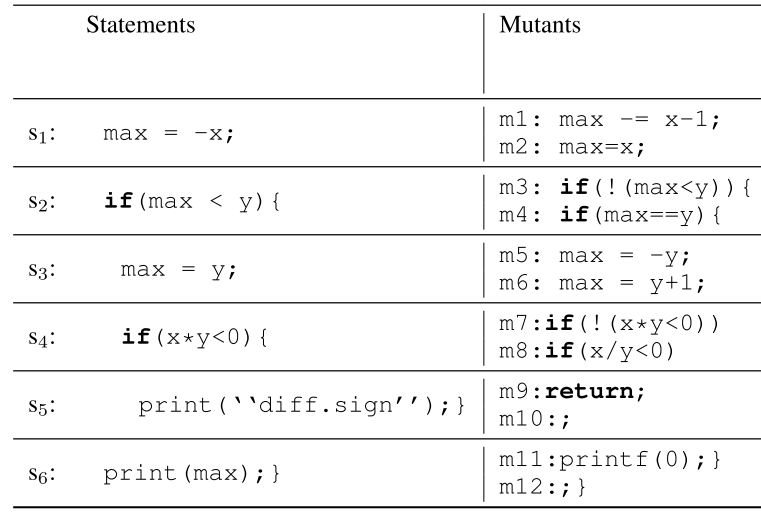
\includegraphics[width=.6\textwidth]{img/mutants.PNG}
	\caption{ نمونه‌ای از جهش‌یافته‌های یک برنامه \cite{moon2014ask}}
	\label{fig:mutant}
\end{figure}
\نام{جاست}{Just} و همکاران در پژوهش خود به بررسی این موضوع پرداخته‌اند که آیا جهش‌یافته‌ها می‌توانند جایگزین مناسبی برای خطاهای واقعی باشند یا خیر\cite{just2014mutants}. در پژوهش‌های گذشته بررسی شده بود که میان جهش‌یافته‌های ساده و پیچیده وابستگی وجود دارد ولی وابستگی میان جهش‌یافته‌های ساده و خطاهای واقعی مشخص نیست. جاست و همکاران دو مجموعه‌ی آزمون برای هر خطا در نظر گرفتند که مجموعه‌ی اول در نسخه‌ی حاوی خطا با موفقیت گذرانده می‌شود. مجموعه‌ی دوم در نسخه‌ی حاوی خطا شکست می‌خورد و در نسخه‌ی رفع خطا با موفقیت اجرا می‌شود. نتایج نشان می‌دهد که مجموعه‌ی آزمون دوم دارای امتیاز جهش بالاتری می‌باشد که نشان می‌دهد هر خطا به یک جهش‌یافته وابستگی دارد. لازم به ذکر است که سعی شده  دو مجموعه‌ی آزمون دارای پوشش یکسانی باشند زیرا پوشش بیشتر می‌تواند امتیاز جهش بیشتر بیانجامد. همچنین مشخص شد که  
73 \lr{\%} 
خطاهای واقعی با جهش‌یافته‌هایی که  با عملگرهای متدوال تولید شده‌اند وابستگی دارند. در این پژوهش خطاهایی که با جهش‌یافته‌ها وابستگی ندارند در سه دسته قرار می‌گیرند : دسته اول نیازمند عملگرهای قوی‌تری هستند، دسته‌ی دوم نیازمند عملگرهای جدیدی هستند و دسته‌ی سوم با جهش‌یافته‌ها وابستگی ندارند.\\
\subsection{مکان‌یابی خطا}
روش‌هایی که از جهش‌یافته‌ها به منظور مکان‌یابی خطا استفاده می‌کنند دارای شباهت‌هایی با روش‌های پیش‌بینی خطا هستند. در هر دوی این روش‌ها از معیارهایی  کد منبع استفاده می‌شود تا احتمال وجود خطا محاسبه شود. دو تفاوت عمده‌ی این دو حوزه این است که اولا در مکان‌یابی خطا از روش‌های یادگیری ماشین استفاده‌ی چندانی نمی‌شود، ثانیا در مکان‌یابی خطا وجود خطا به وسیله شکست مورد آزمون یا گزارش خطا محرز شده است. با توجه به شباهت‌های موجود میان این دو حوزه در ادامه چند مقاله که با استفاده از آزمون جهش خطا را مکان‌یابی کرده‌اند، بررسی می‌کنیم. \\

\نام{موون}{Moon} و همکاران در مقاله‌ی خود بر اساس دو فرض روشی به منظور مکان‌یابی خطا ارائه داده‌اند. فرض اول بیان می‌کند که  در یک برنامه‌ی حاوی خطا جهش و یا اصلاح یک عبارت خطا‌دار نسبت به جهش یک عبارت درست می‌تواند موارد آزمون بیشتری را  با موفقیت بگذراند. فرض دوم  بیان می‌کند که جهش عبارات صحیح نسبت به جهش یک عبارت غلط موجب می‌شود موارد آزمون بیشتری شکست بخورند. بر اساس این دو فرض معیاری به نام \واژه{مشکوک بودن}  ارائه گردیده است که دو فرض را فرموله می‌کند. این معیار بر اساس تعداد شکست و موفقیت موارد آزمون در نسخه‌ی اصلی و جهش‌یافته عمل می‌کند. سپس با رتبه‌بندی عبارات بر اساس این معیار عبارت حاوی خطا مشخص می‌گردد. در این پژوهش روش جدیدی نیز به منظور ارزیابی روش پیشنهادی ارائه شده است که برخی از مشکلات روش پیشین را بر طرف نموده است. در نهایت روش مکان‌یابی ارائه شده با دو روش ارزیابی شده و نتایج نشان می‌دهد فرضیات پژوهش درست بوده‌اند \cite{moon2014ask}. \\

\نام{پاپاداکیس  و تراوون}{Papadakis and Traon} در مقاله‌ی خود به این نکته اشاره کرده‌اند  که استفاده از تحلیل جهش در گذشته به دلیل پر هزینه بودن چندان مورد توجه قرار نمی‌گرفته است اما امروزه با وجود ابزارهای مقیاس پذیر، نمونه گیری و انتخاب جهش می‌توان به خوبی از تحلیل جهش در انجام پژوهش‌های مختلف استفاده کرد\cite{papadakis2015metallaxis}. آنها روشی را برای مکان‌یابی خطا بر اساس دو مشاهده ارائه کرده‌اند. در مشاهده‌ی اول دیده می‌شود که خطای موجود در یک عبارت رفتار مشابهی با جهش در همان عبارت نشان می‌دهد. در مشاهده‌ی دیگر دیده می‌شود که اگر  خطا و جهش در دو عبارت متفاوت باشند رفتار متفاوتی خواهند داشت. منظور از رفتار مشابه موفقیت یا شکست در یک آزمون است. بر اساس این دو مشاهده معیاری برای مشکوک بودن عبارات تعیین می‌گردد. این پژوهش بیان می‌کند که مناسب بودن موارد آزمون تاثیر مستقیمی بر عملکرد روش مکان‌یابی خطا  دارد. همچنین یک مجموعه‌ی کوچک از جهش‌یافته‌ها می‌تواند به اندازه‌ی مجموعه‌ای کامل تاثیر گذار باشد. \\

\subsection{مدل‌های یادگیری و جهش‌یافته‌ها}
 
\نام{هااو}{Hao} و همکاران با ارایه‌ی مجموعه‌ای از معیارها و استفاده از یادگیری ماشین مدلی را ارائه داده‌اند که به وسیله‌ی آن بتوان تشخیص داد علت شکست در آزمون رگرسیون وجود خطا است یا \واژه{منسوخ} شدن یک مورد آزمون\cite{hao2013bug}. هفت معیار ارائه شده در این پژوهش مرتبط با گراف فراخوانی، تغییر در فایل‌ها و تعداد شکست در آزمون‌ها بوده است.  هااو و همکاران به منظور به دست آوردن مجموعه داده‌ی حاوی خطا، به صورت دستی بر اساس استانداردهایی  از پیش تعریف شده خطاهایی را در کد قرار داده‌اند. بدین منظور عباراتی به صورت تصادفی که در سراسر کد محصول قرار دارند انتخاب شدند و به وسیله‌ی عملگرهای جهش خطاهایی تولید شده است. به منظور بدست آوردن آزمون‌های منسوخ شده، مجموعه آزمون‌هایی از نسخه‌ی قبلی برنامه بر روی کد  نسخه‌ی بعدی به کار گرفته شده است. سپس با استفاده از روش \واژه{ارزیابی میان دسته‌ای} به آموزش و آزمایش مدل ساخته شده پرداخته می‌شود. نتایج پژوهش نشان می‌دهد که روش پیشنهادی زمانی که بر روی یک نسخه‌یا نسخه‌های مختلف از یک برنامه اعمال شود نتایج خوبی دارد (80\lr{\%} دقت) اما زمانی که بر روی برنامه‌های مختلف اعمال شود ( مجموعه آموزش از یک برنامه و آزمون بر روی برنامه‌ای دیگر) موثر نیست. نتایج نشان می‌دهد تکنیک‌ها مکان‌یابی خطا نتیجه‌ی مثبتی بر تشخیص نوع خطا که مربوط به محصول است یا آزمون، ندارد.\\
 
\نام{بوئز}{Bowes} و همکاران معیارهایی را مبتنی بر جهش معرفی کردند و  از ترکیب آنها با معیارهای سنتی و شئ‌گرایی، یک مدل پیش‌بینی ساخته شده است\cite{bowes2016mutation}. 8 عملگر جهش در نظر گرفته شده و برای هر یک از آنها یک معیار ایستا (بدون اجرای کد) و چهار معیار پویا ساخته شده و در مجموع 40 معیار جهش ارائه شده است. به این دلیل میان معیار ایستا و پویا تمایز قائل شده‌اند که اگر معیارهای ایستا به تنهایی  پیش‌بینی را بهبود بخشند بدون نیاز به موارد آزمون می‌توان از آنها استفاده کرد، در واقع دامنه‌ی کاربرد روش گسترده‌تر می‌گردد. نتایج پژوهش نشان می‌دهد که استفاده از معیارهای جهش بهبود قابل توجهی را در پیش‌بینی خطا به وجود می‌آورد. همچنین معیارهای پویا و ایستا در کنار یکدیگر توانایی پیش‌بینی مناسبی دارند ولی استفاده‌ی جداگانه از آنها تاثیر چندان مثبتی نخواهد داشت. این پژوهش از دو جنبه حائز اهمیت می‌باشد. یکی اینکه اولین پژوهش در زمینه‌ی پیش‌بینی خطاست که از تحلیل جهش استفاده کرده است. دوم آنکه مشابه‌ترین پژوهش به پژوهش کنونی می‌باشد. 
 
 
 
 
 
 
 
 
 
 
 
 
 
 
 
 
 
 
 
 
 


\section{جمع بندی مطالعات پیشین}
\label{sec:conclustion}
هدف از پیش‌بینی خطا کمک به توسعه‌دهندگان نرم‌افزار و کاهش هزینه‌های نرم‌افزاری می‌باشد. روند پیش‌بینی خطا به این صورت است که با استفاده از مخازن نرم‌افزاری همانند سیستم کنترل نسخه و سیستم ردگیری خطا، اطلاعات کد منبع، خطا و اطلاعات تاریخی پروژه جمع آوری می‌شود. با توجه به معیارهای مختلف داده‌هایی استخراج می‌شود که هر داده دارای برچسب "سالم" یا "حاوی خطا" می‌باشد. قسمتی از این داده‌ها با استفاده از روش‌های یادگیری ماشین، مدل‌های پیش‌بینی خطا را تولید می‌کنند و قسمت دیگر جهت آزمایش مدل به کار گرفته می‌شود.\\

معیارهای متداول در ارزیابی پیش‌بینی دقت و فراخوانی می‌باشند. این معیارها دارای نواقصی هستند. به عنوان مثال مدلی که همه‌ی داده‌ها را خطا دار معرفی می‌کند دارای فراخوانی  برابر یک است و مسلما این مدل کارایی مناسبی ندارد. معیار اف  میانگین هارمونیک دو معیار قبلی است و نواقص آنها را بر طرف می‌کند. یکی از معیار‌های رایج برای مقایسه‌ی مدل‌های یادگیری ماشین مساحت زیر منحنی می‌باشد. هرچه این مساحت بیشتر باشد و منحنی مربوطه سریعتر  در راستای محور عمودی  به یک برسد مدل کارایی بهتری دارد. با استفاده از معیار مساحت زیر منحنی هزینه-اثربخشی می‌توان موثر بودن مدل از نظر هزینه را سنجید. معمولا چند درصد اول از منحنی مربوطه در نظر گرفته می‌شود و مساحت آن محاسبه می‌شود. \\

معیارهای مورد استفاده را می‌توان به سه دسته‌ی معیار سنتی کد، معیار شئ گرایی و معیار فرآیند تقسیم کرد. در برخی از منابع نیز  به دو دسته‌ی کلی معیار کد و معیار فرآیند تقسیم شده‌اند. معیارهای اندازه جزء معیارهای ابتدایی و موثر هستند و معیارهای پیچیدگی و شئ گرایی همبستگی فراوانی با معیارهای اندازه دارند. معیارهای شئ گرایی دارای وابستگی فراوانی با معیار‌های اندازه هستند. با این حال معیارهای شئ گرایی دارای توانایی بیشتری هستند. معیارهای فرآیند از جنبه‌های مختلفی  مانند عدم رکود در تکرار‌های چرخه‌ی تولید نرم‌افزار و موثر بودن از نظر هزینه از سایر معیارها برتری دارد. علی‌رغم توانمندی بالقوه‌ی معیارهای فرآیند در پیش‌بینی خطا، این معیارها در پژوهش‌های کمتری مورد تحقیق قرار گرفته‌اند. \\

در پژوهش‌های مختلف از روش‌های یادگیری ماشین متفاوتی استفاده شده است. در صورتی که هدف پیش‌بینی تعداد خطاها باشد از رگرسیون و در صورتی که هدف پیش‌بینی حاوی خطا بودن باشد از دسته‌بندی استفاده می‌شود. پژوهش \cite{arisholm2010systematic}  نشان داده است که روش دسته‌بندی تاثیر متوسطی بر کارایی پیش‌بینی خطا دارد و انتخاب معیار مهم‌تر است. \\

 در ابتدا از امتیاز جهش برای میزان موثر بودن مجموعه آزمون استفاده می‌شد و سپس کاربردهای دیگری همچون انتخاب، رتبه‌بندی و کمینه کردن مجموعه آزمون پیدا کرده است. همچنین در پژوهش‌های اخیر جهت مکان‌یابی خطا و پیش‌بینی خطا مورد استفاده قرار گرفته است. در پژوهش \cite{just2014mutants} نشان داده شده است که جهش‌یافته‌هایی  که با عملگرهای جهش ساده تولید شده‌اند می‌توانند تا 73 \lr{\%} خطاهای واقعی را شبیه سازی کنند و ازین جهت جایگزین مناسبی برای خطاهای واقعی باشند. 


\begin{table}[H] 
	\centering \caption{جدول مشخصات پژوهش‌ها‌‌ی مرور شده در حوزه‌ی پيش بيني خطا}
	\label{tab:survey}
	\newcolumntype{P}[1]{>{\centering\arraybackslash}m{#1}}
	\renewcommand*{\arraystretch}{1.5}
	\begin{tabular}{|P{1cm}|P{2cm}|P{3cm}|P{1.5cm}|P{2cm}|P{1.5cm}|P{1cm}|}
		\hline
		\hline
		مقاله & معیار   & تکنیک یادگیری &  ریزدانگی &روش ارزیابی & نوع پروژه‌ها&‌ زبان پروژه‌ها   \\
		\hline
		\hline
		
		\cite{ostrand2010programmer}
		 & فرآیند - سنتی & \lr{NBR} & فایل & مشابه \lr{AUCEC} & خصوصی & جاوا \\
		 \hline
		
		\cite{rahman2013and}
	&	فرآیند - سنتی - شئ‌گرایی & 
		\lr{Naive Bayes - Logestic Regression - SMV - J48}
		& فایل &  \lr{AUC - AUCEC - F-Measure} & متن باز& جاوا \\

		\hline
		\cite{bowes2016mutation}
		& سنتی - شئ‌گرایی & 
			\lr{Naive Bayes - Logestic Regression - Random Forest - J48} 
			&
			کلاس & غیره & متن باز & جاوا \\
		\hline
		\cite{malhotra2014comparative} &
		سنتی &  
		\lr{LR - ANN - DT - SVM - CCN - GMDH - GEP} & \lr {NA} & \lr {AUC - Precision} & 
		متن باز & سی \\
		\hline
		
		\cite{xia2016predicting} &
		سنتی - فرآیند &
		\lr{Naive Bayes - DT - kNN - RF} & سیستم & \lr {AUC - Precision - Recall - F-Measure} & 
		متن باز & اندروید \\
		\hline
		\cite{kumar2017emprical} &
		سنتی - شئ‌گرایی &
		\lr{LR - ANN - RBFN } & کلاس & \lr {Accuracy - F-Measure} & 
		متن باز & جاوا \\
		\hline
		
		
		
	
\end{tabular}
\end{table}














\chapter{معیارهای جهش و فرآیند}
 
\label{sec:method}
با  مطالعات مروری انجام شده نقاطی از این حوزه که نیازمند پژوهش بیشتر هستند تا بتوان به وسیله‌ی آن به ارائه‌ی روشی کاراتر در پیش‌بینی خطا پرداخت مشخص شد. مقاله‌ی \cite{bowes2016mutation} اولین مقاله‌ای است که  یک  روش پیش‌بینی خطا با استفاده از تحلیل جهش ارائه نموده  است و این موضوع نیازمند تحقیق بیشتر است. از طرف دیگر بر طبق مقاله‌ی \cite{radjenovic2013software} استفاده از معیارهای فرآیند علی‌رغم توانایی بالقوه‌ای که در پیش‌بینی خطا دارند، در پژوهش‌های کمتری مورد بررسی قرار گرفته‌اند. یکی از دلایل آن می‌تواند نو ظهور بودن این معیارها نسبت به سایرین باشد. معیارهای فرآیند از جنبه‌های مختلف نیز از سایر معیار‌ها برتری دارند \cite{rahman2013and}. \\
این پژوهش قصد دارد سه رویکرد  پیشنهادی را به منظور بهبود پیش‌بینی خطا بررسی کند.  این رویکردها عبارتند از:
\begin{enumerate}
\item
در این رویکرد معیارهای جهش و معیارهای فرآیند در کنار یکدیگر استفاده می‌شوند و به وسیله‌ی آنها پیش‌بینی انجام می گیرد. این دو دسته معیار در پژوهش‌های گذشته مطرح شده‌اند اما تاکنون در کنار یکدیگر قرار نگرفته‌اند.
\item
معیارهای جدیدی مطرح می‌شوند که مبتنی بر مفاهیم آزمون جهش و فرآیند توسعه‌ی نرم‌افزار است.
\item
معیارهای جدیدی مطرح می‌شوند که با کمک مفاهیم جهش سعی در بهبود معیارهای فرآیند دارند.
\end{enumerate}

\section{معیارهای جهش و فرآیند}

این رویکرد با توجه به مقاله‌ی \cite{bowes2016mutation} مطرح شده که در آن بررسی به کارگیری معیارهای جهش و فرآیند را در پژوهش‌های آتی توصیه می‌کند.  همچنین  معیار جهش یک معیار  مرتبط با کد است. مقاله‌ی \cite{rahman2013and}  بیان می‌کند که معیارهای کد ایستا هستند و تمایل دارند که یک موجودیت را در انتشارهای متوالی حاوی خطا معرفی کنند. حال شرایطی را در نظر بگیرید که که امتیاز جهش در یک موجودیت کم باشد و دلیل آن کافی نبودن مجموعه آزمون باشد چراکه توسعه‌دهندگان از درست بودن کد اطمینان دارند یا اینکه پس از انتشارهای متوالی خطاها بر طرف شده است. چنین موجودیتی حاوی خطا نیست اما با توجه به معیار جهش خطا‌خیز است. با در نظر گرفتن معیارهای فرآیند در مورد این موجودیت که نشان می‌دهند پایدار و بدون تغییر است از میزان خطا‌خیز بودن آن کاسته می‌شود و انتظار می‌رود کارایی مدل پیش‌بینی بهبود یابد. 
برای پاسخ به این پرسش مجموعه معیارهای جهش  از پژوهش \cite{bowes2016mutation}  و معیارهای فرآیند از پژوهش \cite{rahman2013and} انتخاب می‌شوند. در جداول  \ref{tab:process-metircs} و \ref{tab:mutation-metircs} معیارهای مورد نظر آورده شده است و در ادامه معرفی شده و  \\
\begin{table}[H] 
	\renewcommand*{\arraystretch}{1}	
	\centering \caption{معیارهای فرآیند 
		\cite{rahman2013and}}
	\label{tab:process-metircs}
	\newcolumntype{C}{>{\centering\arraybackslash} m } 
	
	\begin{tabular}{|c|c|}
		
		\hline
		\hline
		نام معیار  & توضیح
		\\
		\hline
		\hline
		\lr{COMM } & تعداد ثبت در سیستم کنترل نسخه
		\\
		\hline
		\lr{ADEV} & تعداد توسعه‌دهندگان 
		فعال
		\\ 
		\hline
		\lr{DDEV} & تعداد توسعه‌دهندگان 
		متفاوت
		\\ 
		\hline
		\lr{ADD} &  مقدار نرمال‌سازی شده‌ی تعداد خطوط اضافه شده
		\\ 
		\hline
		\lr{DEL}  & مقدار نرمال‌سازی شده‌ی تعداد خطوط حذف شده
		\\ 
		\hline
		\lr{OWN} &  درصد خطوطی که مالک فایل مشارکت کرده
		\\ 
		\hline
		\lr{MINOR} & تعداد مشارکت‌کنندگان جزئی
		\\ 
		\hline
		\lr{NCOMM} & تعداد ثبت‌های همسایگان
		\\ 
		\hline
		\lr{NADEV} & تعداد توسعه‌دهندگان فعال همسایگان
		\\ 
		\hline
		\lr{NDDEV} & تعداد توسعه‌دهندگان متمایز همسایگان
		\\ 
		\hline
		\lr{OEXP} & تجربه‌ی مالک فایل
		\\ 
		\hline
		\lr{AEXP} & تجربه‌ی تمام مشارکت‌کنندگان
		\\ 
		\hline
		
	\end{tabular}
\end{table}

\begin{table}[H] 
	\renewcommand*{\arraystretch}{1}	
	\centering \caption{معیارهای جهش 
		\cite{bowes2016mutation}}
	\label{tab:mutation-metircs}
	\newcolumntype{C}{>{\centering\arraybackslash} m } 
	
	\begin{tabular}{|c|c|}
		
		\hline
		\hline
		نام معیار &  توضیح
		\\
		\hline
		\hline
		\lr{MuNOM } &   تعداد جهش‌یافته‌های تولید شده
		\\
		\hline
		\lr{MuNOC} &   تعداد جهش‌یافته‌های پوشش‌داده شده توسط آزمون‌ها
		\\
		\hline
		\lr{MuNMS} &   امتیاز جهش‌یافته‌های تولید شده
		\\
		\hline
		\lr{MuNMSC} &   امتیاز جهش‌یافته‌های پوشش‌داده شده توسط آزمون‌ها
		\\
		\hline
		
	\end{tabular}
\end{table}
از آنجا که  در این پژوهش پیش‌بینی‌ها در سطح فایل انجام شود، معیارها برای هر فایل جداگانه محاسبه می‌شوند. در ادامه هر یک از این معیارها معرفی و نحوه‌ی محاسبه‌ی آن‌ها بیان می‌شود.\\

\begin{itemize}
\item
\textbf{تعداد ثبت در سیستم کنترل نسخه:}
 تعداد ثبت‌هایی که در آن فایل مورد نظر در طول انتشار قبلی تاکنون تغییر کرده است. برای محاسبه ی آن لازم است که تمام ثبت‌های پروژه بین ثبت کنونی و \واژه{انتشار} قبلی بررسی شود و ثبت‌هایی که در آن این فایل تغییر کرده‌اند شمرده شوند.
 \item
\textbf{تعداد توسعه‌دهندگان 
	فعال:}
 تعداد توسعه‌دهندگانی که در طول انتشار قبلی تا کنون (زمان ثبت) فایل را تغییر داده‌اند. لازم است ثبت‌های موجود در باز‌ه‌ی زمانی خواسته شده بررسی شود و آنها که فایل مورد نظر را تغییر داده‌اند انتخاب شوند. نام کسانی که ثبت را انجام داده‌اند بازیابی شود و تعداد نامهای متمایز شمرده شود. 
 \item
 \textbf{تعداد توسعه‌دهندگان	متمایز:}
 مشابه معیار قبلی با این تفاوت که در طول انتشار محاسبه نمی‌شود. بلکه از ابتدای پروژه تا زمان ثبت در نظر گرفته می‌شود. 
\item
\textbf{مقدار نرمال‌سازی شده‌ی تعداد خطوط اضافه شده:}
این معیار تعداد خطوط اضافه شده در یک فایل را در طول انتشار قبلی می‌شمارد. سپس جهت نرمال سازی آنرا بر تعداد کل خطوط اضافه شده در پروژه در طول انتشار قبلی تقسیم می‌کند. برای بدست آوردن تعداد خطوط اضافه شده در یک فایل هر ثبت تسبت به ثبت قبلی مقایسه می‌شود و تعداد خطوط اضافه شده جمع زده می‌شود.
\item
\textbf{مقدار نرمال‌سازی شده‌ی تعداد خطوط حذف شده:}
مشابه معیار قبلی می‌باشد. 
\item
\textbf{تعداد خطوطی که مالک فایل مشارکت کرده:}
 درصد خطوطی  از فایل، در  ثبت مورد نظر  که به مالک فایل تعلق دارد. مالک فایل کسی است که در آن لحظه از زمان بیشترین تعداد خطوط موجود در فایل به او تعلق دارد. ابتدا نویسنده‌ی هر خط مشخص می‌شود سپس برای هر تویسنده تعداد خطوطی که به وی تعلق دارد شمرده می‌شود. تعداد خطوط مالک فایل بر تعداد خطوط فایل تقسیم می‌گردد.
\item
\textbf{تعداد مشارکت‌کنندگان جزئی:}
توسعه‌دهنده‌ی جزئی کسی است که کمتر از ۵٪ خطوط موجود در فایل به او تعلق داشته باشد. بدین منظور نویسنده‌ی هر خط مشخص می‌شود. تعداد خطوط هر نویسنده شمرده می‌شود و بر تعداد خطوط فایل تقسیم می‌شود. سپس تعداد نویسندگانی که کمتر از ۵٪ مشارکت داشته‌اند شمرده می‌شود. 
\item
\textbf{تعداد ثبت‌های همسایگان}
 میانگین وزن دهی شده تعداد ثبت‌های همسایگان فایل از انتشار قبلی تا کنون را اندازه‌گیری می‌کند. همسایگان یک فایل در یک ثبت، فایل‌هایی هستند که در آن نسخه از برنامه تغییر کرده‌اند. در‌واقع در هر ثبت از برنامه تعدادی فایل نسبت به ثبت قبلی تغییر کرده‌اند که این فایل‌ها همسایه‌ی یکدیگر محسوب می شوند. نحوه‌ی وزن دهی نیز به این صورت است که هرچقدر یک فایل تعداد دفعات بیشتری را در طول انتشار با فایل مورد نظر همسایه شده باشد وزن بیشتری می‌یابد. برای محاسبه ابتدا همسایگان فایل در ثبت  و تعداد دفعاتی که  در طول انتشار همسایه شده‌اند مشخص می‌شوند. سپس برای هر فایل همسایه، معیار تعداد ثبت در سیستم کنترل نسخه محاسبه می‌شود. هر معیار در تعداد دفعاتی همسایگی ضرب می‌شود و با هم جمع زده می‌شوند. در انتها بر تعداد کل دفعات همسایگی همسایگان تقسیم می‌شود. 
\item
\textbf{تعداد توسعه‌دهندگان فعال همسایگان:}
مشابه معیار قبلی عمل می‌شود با این تفاوت که معیار توسعه‌دهندگان فعال در نظر گرفته خواهد شد.

\item
\textbf{تعداد توسعه‌دهندگان متمایز همسایگان:}
مشابه معیار قبلی عمل می‌شود با این تفاوت که معیار توسعه‌دهندگان متمایز در نظر گرفته خواهد شد.
\item
\textbf{تجربه‌ی مالک فایل:}
 ابتدا لازم است که نحوه ی محاسبه تجربه را تعریف کنیم. هر چقدر یک فرد تعداد تغییرات بیشتری را در یک پروژه انجام دهد تجربه بیشتری را در آن پروژه دارد و ثبت را می‌توان به ایجاد تغییر تعبیر کرد. برای محاسبه‌ی معیار ابتدا مالک فایل مشخص می شود. سپس تعداد ثبت‌هایی که مالک فایل از ابتدای پروژه تا زمان مورد نظر انجام داده، شمرده می شود.
\item
\textbf{تجربه‌ی تمام مشارکت‌کنندگان:}
تمام مشارکت‌کنندگان در فایل تا زمان ثبت مورد نظر یافت می‌شوند. برای هر یک مشابه معیار قبلی تجربه، محاسبه می‌شود و از مقدار تجربه‌ها میانگین هندسی گرفته می‌شود. 

\end{itemize}


%%%%%%%%%%%
\section{معیارهای جهش مبتنی بر فرآیند}
در پاسخ به سوال دوم چهار معیار زیر مطرح می‌شود:
\begin{enumerate}
	
	\item  
	\textbf{
		تعداد جهش‌یافته‌های تولید شده‌ی جدید نسبت به نسخه‌ی قبلی برنامه: }همانطور که در مقاله‌ی \cite{just2014mutants} مطرح شده جهش‌یافته‌ها جایگزین خوبی برای خطاهای واقعی می‌باشند. زمانی که تعداد جهش‌یافته‌های جدید زیاد باشد یعنی تغییراتی که خطا‌خیز‌ترهستند بیشتر است. 
	\item 
	\textbf{
		تعداد جهش‌یافته‌های متمایز در تمام نسخه‌های قبلی:} این معیار نشان می‌دهد موجودیت مورد بررسی به چه میزان سابقه‌ی تغییراتی را دارد که احتمال بروز خطا را افزایش می‌دهد.
	
	\item 
	\textbf{
		میزان تغییرات مثبت امتیاز جهش دو به دو در تمام نسخه‌های قبلی:}
	تغییرات امتیاز جهش نشان از تغییرات در برنامه و آزمون‌های نرم‌افزار است.     این معیار نشان می‌دهد این تغییرات به چه میزان در جهت بهبود کیفیت نرم‌افزار بوده. چراکه امتیاز بالاتر جهش نشان از کیفیت بهتر آزمون‌ها و در نتیجه نرم‌افزار است. 
	\item 
	\textbf{
		میزان تغییرات منفی امتیاز جهش در تمام نسخه‌های قبلی:}
	این معیار مشابه معیار سوم عمل می‌کند با این تفاوت که میزان تغییرات در خلاف جهت بهبود نرم‌افزار را می‌سنجد. 	
	
\end{enumerate}
با استفاده از مجموعه داده‌ی فراهم شده دو مدل پیش‌بینی ساخته می‌شود. یکی با استفاده از معیارهای فرآیند به تنهایی و دیگری با استفاده از معیارهای مطرح شده. سپس با استفاده از روش‌های ارزیابی مطرح شده در قسمت \ref{subsec:eval}  دو مدل مقایسه می‌شوند.\\

\section{معیارهای ترکیبی جهش-فرآیند}
پرسش سوم با توجه به مطالب گفته شده در مقاله‌ی \cite{rahman2013and} مطرح شده که بیان می‌کند معیارها هر چقدر هم که پویا باشند (دچار رکود نشوند، مانند معیارهای فرآیند) زمانی در پیش‌بینی خطا مفید هستند که همراه با ایجاد خطا باشند.  دو معیار مطرح در میان معیارهای فرآیند تعداد خطوط اضافه شده و حذف شده است. با توجه به تعداد جهش‌یافته‌هایی که  اضافه  و یا حذف هر خط ایجاد می‌کند، اضافه یا کم شدن خطوط وزن دهی می‌شود. دو معیار جدید به صورت زیر ساخته می‌شود و تاثیر آنها بر کارایی مشابه پرسش اول و دوم سنجیده می‌شود. \\
\begin{latin}
	
	$M_1 =\ number\ of\ lines\ added\ \times \ number\ of\ muatants\ derived$\\
	
	$M_2 =\ number\ of\ lines\ deleted\ \times \ number\ of\ mutants\ derived$\\
\end{latin}


\chapter{مورد مطالعاتی}
در این فصل مطالعه‌ی موردی بر روی مجموعه‌داده‌ی \lr{defects4j} \cite{Just:2014:DDE:2610384.2628055} انجام می‌گیرد. ابتدا نحوه‌ی کلی برپایی آزمایش شرح داده می‌شود و سپس چگونگی استخراج معیارها و پیاده‌سازی ارمایش توضیح داده خواهد شد. 
\section{طراحی آزمایش}
به منظور ارزیابی رویکردهای گفته شده لازم است که برای مجموعه معیارهای هر رویکرد مدلهای پیش‌بینی ساخته شود و هر عملکرد هر مدل نسبت به پژوهش‌های گذشته مقایسه شود. به این ترتیب ابتدا لازم است از مجموعه‌داده‌ی فراهم شده معیارهای بیان شده در فصل \ref{sec:method} استخراج شوند. مجموعه‌داده‌ی \lr{defects4j} که در قسمت‌های آتی معرفی می‌شود شامل اطلاعات خطا در چندین فایل است و به همین تعداد، فایل بدون خطا در ثبت و پروژه‌ی متناظر به طور تصادفی انتخاب می‌گردد. برای فایلهای حاوی خطا و سالم، معیارها استخراج می‌شود. معیارهای استخراج شده  برای هر فایل به عنوان بردار ویژگی در مدلهای دسته‌بندی عمل می‌کند. مدلهای دسته‌بندی به منظور پیش‌بینی حاوی خطا بودن ساخته می‌شود و عملکرد آنها مقایسه می‌گردد. مدلهایی که با هم مقایسه می‌شود در الگوریتم و \واژه{پیکربندی} یکسان هستند و تنها تفاوت آنها در معیارهای استفاده شده به منظور یادگیری است. بدین ترتیب تاثیر معیارها بر پیش‌بینی خطا سنجیده می‌شود. 

\section{ آشنایی با ابزارها و مجموعه داده}
این قسمت به معرفی ابزارهای استفاده شده در این پژوهش می‌پردازد. آشنایی با این ابزارها به درک هرچه بهتر  نحوه‌ی استخراج معیارها  و روند آزمایش کمک می‌کند.

\subsection{مجموعه داده \lr{defect4j}}
 مجموعه‌‌داده‌ی انتخابی به منظور انجام مورد مطالعاتی لازم است که دارای ویژگی‌های زیر باشد:
 \begin{itemize}
 	\item
 	اطلاعات خطاهای پروژه وجود داشته باشد و این اطلاعات نشان دهد که خطا متعلق به کدام فایل در کدام ثبت است. 
 	\item
 	پروژه‌ها متن-باز باشد تا بتوان با استفاده از کد منبع آنها معیارها را استخراج نمود.
 	\item
 	برای پروژه‌ها موارد آزمون مناسب وجود داشته باشد تا بتوان معیارهای جهش را استخراج کرد.
 \end{itemize}
 در میان مجموعه‌داده‌های موجود مجموعه‌داده‌ی \lr{defects4j} تنها موردی است که تمام ویژگی‌ها را دارد.\\
 
این مجموعه شامل  شش پروژه می‌باشد که پنج مورد از آن‌ها مربوط به شرکت \نام{آپاچی}{Apache} است و دیگری نرم‌افزار jfreechart است که به شرکت خاصی تعلق ندارد. این پروژه‌ها  \واژه{متن-باز} هستند و با استفاده از نرم‌افزارهای کنترل نسخه‌ی گیت و svn می‌توان به کدهای آن‌ها در طول فرآیند توسعه‌ی آنها دسترسی پیدا کرد.
مجموعه‌داده‌ی \چر{defect4j} به صورت یک \واژه{چهارچوب} ارائه شده است که کارهایی بیش از نگهداری اطلاعات درباره‌ی پروژه‌ها انجام می‌دهد. مهم‌ترین  کارهایی که می‌توان به وسیله‌ی این ابزار انجام داده عبارت است در جدول زیر آمده است. 


\begin{table}[H] 
	\renewcommand*{\arraystretch}{1.3}	
	\centering \caption{عملیات‌های موجود در \چر{defects4j}  }
	\label{tab:defects4j-ops}
	\newcolumntype{C}{>{\centering\arraybackslash} m } 
	\begin{tabular}{ |c|c|}
		
		\hline
		\hline
		نام عملیات  & توضیح
		\\
		\hline
		\hline
		\lr{info } &   نمایش پیکربندی یک پروژه‌ی خاص یا خلاصه‌ی یک خطای خاص
		\\
		\hline
		\lr{checkout} &   وارسی یک نسخه‌ی حاوی خطا یا تعمیر شده از پروژه
		\\
		\hline
		\lr{compile} &   کامپایل کدهای و آزمون‌های نوشته شده توسط توسعه‌دهندگان
		\\
		\hline
		\lr{test} &   اجرای یک آزمون یا مجموعه‌ی آزمون در یک نسخه‌ی حاوی خطا یا تعمیر شده از پروژه
		\\
		\hline
		\lr{mutation} &   اجرای تحلیل جهش در یک نسخه‌ی حاوی خطا یا تعمیر شده از پروژه
		\\
		\hline
		
	\end{tabular}
\end{table}

این ابزار در اجرای عملیات‌های بالا دارای محدودیت است و تنها آن‌ها را بر روی ثبت‌های از پیش تعیین شده انجام می‌دهد. ثبت‌های از پیش تعیین شده شامل ثبت‌های حاوی خطا و تعمیر آن خطا می‌باشد. در جدول زیر اطلاعات مربوط به تعداد خطاهای هر پروژه آمده است. 

\begin{table}[H] 
	\renewcommand*{\arraystretch}{1.3}	
	\centering \caption{پروژه‌های موجود در \چر{defects4j}  }
	\label{tab:defects4j-bugs}
	\newcolumntype{C}{>{\centering\arraybackslash} m } 
	\begin{tabular}{ |c|c|c|}
		
		\hline
		\hline
	نام مختصر &	نام کامل  & تعداد خطا
		\\
		\hline
		\hline
		\lr{Chart } & JFreeChart &	26
		\\
		\hline
		\lr{Closure} & \lr{Closure compiler}	& 133
		\\
		\hline
		\lr{Lang} &   \lr{Apache commons-lang} &	65
		\\
		\hline
		\lr{Math} &  \lr{Apache commons-math} &	106
		\\
		\hline
		\lr{Mockito} &   Mockito &	38
		\\
		\hline
		Time & Joda-Time &	27
		\\
		\hline
		
	\end{tabular}
\end{table}


به منظور نصب و راه اندازی این ابزار ابتدا از صفحه ی github آن پروژه بر روی  PC ، کلون می شود. سپس یک script باید اجرا کرد تا سایر تعلقات پروژه دانلود شود. این تعلقات شامل مخزن نرم افزاری مربوط به این این شش پروژه است که کدهای پروژه ها در آن قرار دارد. نکته ی قابل توجه در این پروژه این است بجز  دستور info سایر دستورات عملیاتهای مربوط را بر روی کامپیوتر کاربر انجام می‌دهند و خروجی را نمایش می‌دهند نه اینکه از یک پایگاه داده اطلاعات صرفاً بارخوانی شوند. 
در نیازمندی های این ابزار اشاره شده که باید از جاوا نسخه ی ۷ استفاده شود. اما مسأله ای که به آن اشاره نشده توزیع کننده ی جاوا است. جاوا دو توزیع کننده ی عمده دارد. یکی OpenJDK و دیگر Oracle. در ابتدا از نسخه ی openJDK استفاده شد زیرا نصب آن در linux ساده‌تر است و همچنین oracle به ایرانیان اجازه ی دانلود نمی دهد. اما با openJDK ابزار defects4j و ابزارهایی که به آن وابسته است به خوبی کار نمی کنند. به عنوان مثال برخی مجموعه تست ها که باید بدون خطا اجرا شوند به دلیل نبود dependency های لازم با شکست مواجه می شوند. این مسأله موجب سردرگمی و صرف مدت زمانی تا حل آن شد. 
راه ارتباط با این ابزار command line‌ می‌باشد و نمونه‌ ای از دستورات قابل استفاده در این ابزار  در شکل  \ref{fig:d4j-info-command} است که این دستور اطلاعات مربوط به پروژه ی Lang خطای شماره ی یک را خواهد داد. 
\begin{latin}
	\flushleft
defects4j info -p Lang -b 1
\end{latin}

\begin{figure}[H]
	\centering
	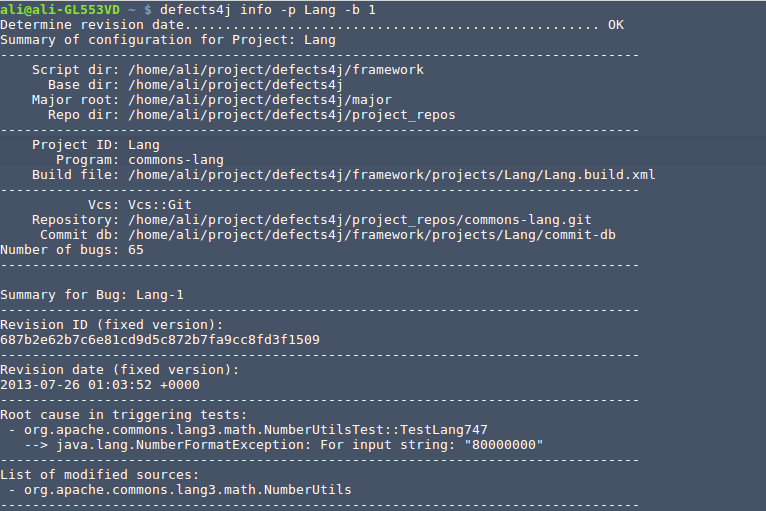
\includegraphics[width=.8\textwidth]{img/case_study/d4j-info-commadn.png}
	\caption{اجرای دستور info در \lr{defects4j}}
	\label{fig:d4j-info-command}
\end{figure}

\subsection{ابزار Major}

این ابزار جهت تولید جهش یافته و تحلیل جهش استفاده می شود. در ابتدا تصمیم بر این بود از ابزار دیگری به نام PIT استفاده شود ولی ابزارdefect4j از major استفاده می‌کند بنابرین به دلیل سازگاری با D4j و نیز قابلیت‌های منحصر به فرد این ابزار تصمیم به استفاده از Major  گرفته شد. چند مورد از ویژگی‌ها عبارتند از :
\begin{itemize}

\item
 راحتی استفاده: قابلیت تعامل از روشهای مختلف مانندcommand lineِ، بکارگیری به وسیله ی ابزار build ant و دستورات کم نسبت به PIT
\item
 مجموعه عملگرهای کاملتر
\item
 راحتی در پیکر بندی : امکان انجام تحلیل تنها برای یک کلاس یا تابع، تنظیمات راحت و کامل جهت مشخص کردن مجموعه عملگرها
\end{itemize}
لازم به ذکر است که این ابزار از compiler‌ مخصوص به خود جهت کامپایل برنامه و ساخت جهش یافته استفاده می‌کند که گسترش یافته ی یک کامپایلر جاوا است. 
البته در انتها مشخص شد که این برنامه کاستی هایی هم دارد از جمله کامل نبود مستندات برای بکارگیری پیشرفته و خطاهایی که در قسمت مربوطه به آن‌ها اشاره خواهد شد. 
استفاده از این ابزار را می‌توان در سه مرحله خلاصه کرد :
\begin{enumerate}
\item

پیکربندی تولید جهش یافته به وسیله MML script: این ابزار برای مشخص نمودن اینکه از چه عملگرهای استفاده شود و آن‌ها در چه محل هایی از برنامه به کار گرفته شوند یک زبان ساده ابداع کرده است به نام MML که یک کامپایلر نیز دارد. ابتدا کد mml نوشته می‌شود سپس با mmlc کامپایل می‌شود و نتیجه به عنوان یکی از پارامترها به در هنگام فراخوانی ابزار ارسال می شود. نمونه‌ای از این کد در شکل \ref{fig:major-mml} آمده است. 

\begin{figure}[H]
	\centering
	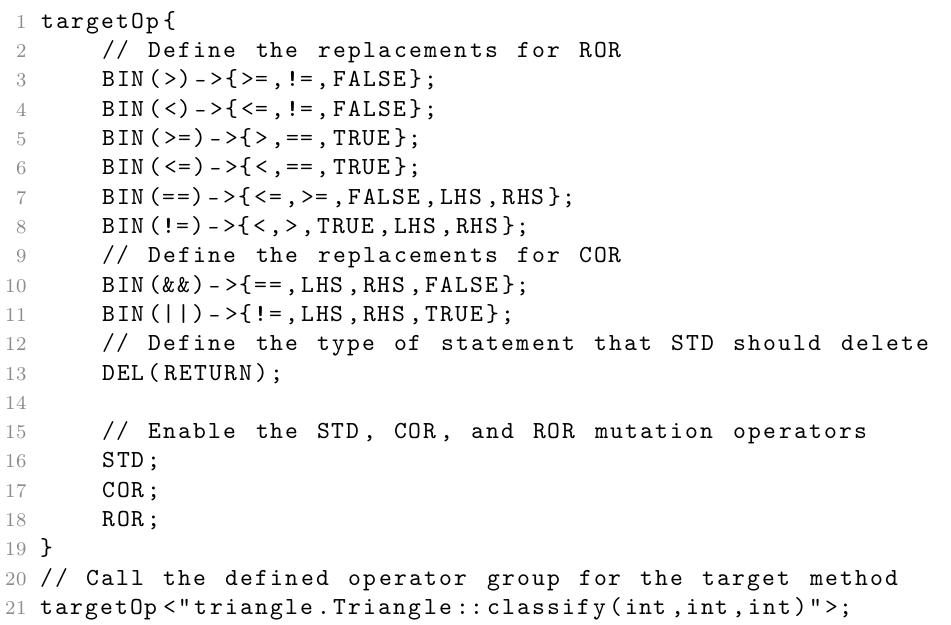
\includegraphics[width=.8\textwidth]{img/case_study/major-mml.png}
	\caption{نمونه کد MML در Major}
	\label{fig:major-mml}
\end{figure}
\item 	
تولید جهش یافته ها: برای این منظور می‌توان از command line یا فایل build.xml مربوط به پروژه استفاده کرد که روش دوم مورد استفاده قرار گرفت. برای این منظور لازم است که یک قطعه کد به شکل زیر به فایل build.xml اضافه شود. و سپس برنامه کامپایل شود. حاصل به شکل زیر خواهد بود که نشان می‌دهد ۸۶ جهش یافته تولید شده است. همچینین ابزار یک فایل به نام mutation.log تولید می‌کند که نشان می‌دهد چه جهش یافته هایی در کجا تولید شده اند. 

\begin{figure}[H]
	\centering
	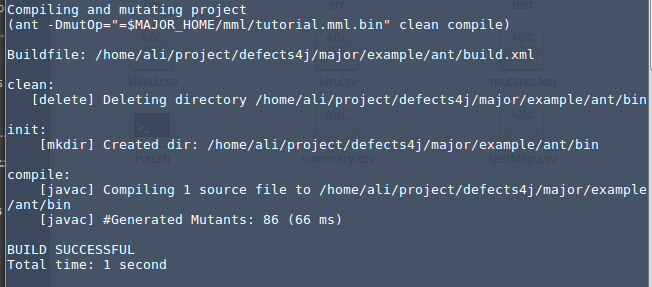
\includegraphics[width=.8\textwidth]{img/case_study/major-mutant.png}
	\caption{نمونه کد MML در Major}
	\label{fig:major-mutant}
\end{figure}

\begin{figure}[H]
	\centering
	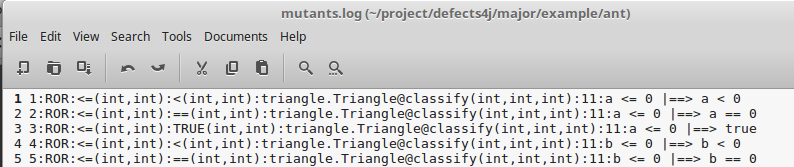
\includegraphics[width=.8\textwidth]{img/case_study/major-log.png}
	\caption{نمونه کد MML در Major}
	\label{fig:major-log}
\end{figure}

\item
 اجرای تحلیل جهش : در این قسمت نیز قطعه کدی به فایل build.xml اضافه می‌شود و سپس فایل اجرا می شود. در اجرا ابتدا فایل‌های تست کامپایل می‌شود و سپس هر مجموعه تست بر روی جهش یافته هایی که تا کنون کشته نشده‌اند اجرا می شود. در پایان نتایج را در خروجی چاپ می کند. همچنین نتایج را در فایلهای با پسوند csv قرار می دهد. نمونه‌ای از اجرای تحلیل جهش و فایلهای خروجی در زیر آمده است:
 
 \begin{figure}[H]
 	\centering
 	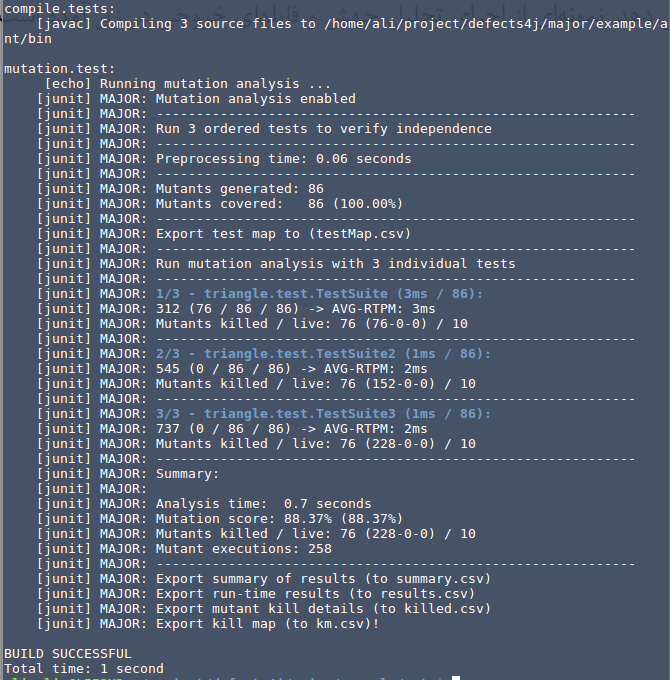
\includegraphics[width=.8\textwidth]{img/case_study/major-analysis.png}
 	\caption{نمونه کد MML در Major}
 	\label{fig:major-analysis}
 \end{figure}
 
 \begin{figure}[H]
 	\centering
 	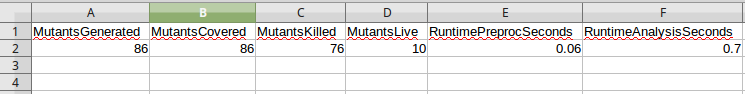
\includegraphics[width=.8\textwidth]{img/case_study/major-results.png}
 	\caption{نمونه کد MML در Major}
 	\label{fig:major-results}
 \end{figure}

\end{enumerate}


\subsection{کتابخانه‌ی Jgit}
این کتابخانه جهت کار با مخازن نرم افزاری از نوع git به کار گرفته می‌شود و به زبان جاوا است. تمام عملیات های مهم و اساسی که در نرم‌افزار اصلی git وجود دارد در این کتابخانه نیز قابل انجام است. مشکلی که کار با این کتابخانه دارد نبود منابع آموزشی به اندازه ی کافی است. چراکه کاربران زیادی ندارد و آموزش‌های ابتدایی معمولاً نیازهایشان را بر طرف می کند. 
\subsection{چهارچوب Hibernate }
به وسیله ی این چارچوب می‌توان  اشیاء موجود در برنامه ی جاوا را به داده‌های موجود در پایگاه داده تبدیل کرد. اصطلاحاً به این ابزار ها ORM (object relational mapping)  می گویند. در ابتدا تصمیم بر این بود که داده‌های بدست آمده در فایل متنی ذخیره شوند و در هنگام نیاز آن‌ها خوانده شوند یا همه ی اشیاء با هر بار اجرا ساخته شوند نکات زیر سبب شد که هزینه ی اول کار با پایگاه داده و مزایای بلند مدت آن به سادگی استفاده از فایل متنی ترجیح داده شود:
۱- هر بار ساخت اشیاء با اجرای برنامه بسیار زمانبر است و اتلاف وقت زیادی دارد
۲- لازم است برای اطمینان از درستی برنامه، داده‌ها در قالب جداولی به صورت چشمی کنترل شوند
۳- فراخوانی و جستجو در پایگاه داده سریع است و کارایی بالا می‌رود
۴- نگهداری از برنامه در دراز مدت راحت‌تر خواهد بود و خوانایی کدها بیشتر خواهد بود چرا که کار با پایگاه داده دارای اصول مشخصی است و سایرین از آن اطلاع دارند اما فایل متنی اینگونه نیست

\section{نکات پیاده‌سازی پروژه}

پیاده‌سازی پروژه در زبان جاوا انجام گرفت. یکی از نکات مهم و قابل توجه در پیاده‌سازی این پروژه این است که تمام مراحل انجام کار  به طور کاملاً خودکار انجام شود و در هیچ مرحله‌ای نیاز به دخالت عامل خارجی  ندارد بجز پیکربندی اولیه مانند آدرس پایگاه داده. همچنین در تمام مراحل سعی شده است که تمام اصول لازم در طراحی معماری نرم‌افزار به کار گرفته شود و نیازمندی‌های کیفی پروژه نیز مد نظر قرار گیرد. این نیازمندی‌ها شامل موارد زیر است:
\begin{enumerate}
\item 
\واژه{کارایی} : جهت پاسخ به این نیازمندی از پایگاه داده استفاده شده است.
\item
قابلیت نگهداری: این قابلیت از سایرین بیشتر حائز اهمیت است. زیرا پروژه های پروژهشی خود به صورت مستقیم کاربران عمومی ندارند و از این جهت نیازمند کارایی بالا یا رابط گرافیکی کاربر پسند نیستند. استفاده آن‌ها معمولاً در گسترش آن‌ها توسط سایر محققین است که راه را ادامه خواهند داد. 
\begin{itemize}
\item

 برای پاسخ به این نیازمندی اصول مربوط به کدنویسی  در فصل سوم و چهارم کتاب  \cite{martin2009clean} به کار گرفته شده است.
 \item
 از الگوهای نرم افزاری پر کاربرد مانند \نام{اداپتور}{Adaptor}،  \نام{فکتوری}{Factory} و \نام{سینگلتون}{Singelton} استفاده شده است.
 \item
 به منظور جلوگیری از قطعه کد تکراری از وراثت و توابع \واژه{عمومی} استفاده شده است. همینطور عمق وراثت از عدد ۳ بیشتر نشده است زیرا وراثت عمیق از خوانایی کد می‌کاهد و محل اشتباه خواهد بود. 
\end{itemize}
\item
امنیت: از آنجا که پروژه قرار نیست به استفاده ی عموم برسد و کاربران عمل متخاصمانه‌ای انجام نخواهند داد   به نوع خاصی از امنیت  نسبت به انواع متداول دارد.  باید روند توسعه‌ی پروژه دارای امنیت باشد. از این نظر که کدها مفقود نشوند یا در صورت اشتباه در توسعه بتوان پروژه را به حالت قبل بازگرداند. در این راستا کدهای پروژه در مخزن نرم افزاری از نوع گیت نگهداری شده که یک مخزن در کامپیوتر شخصی و دیگری در سایت \نام{بیت‌باکت}{Bitbucket - \url{https://bitbucket.org/alimohebbi/bug_predict }} 
قرار دارد. مزیت این سایت نسبت به گیت‌هاب این است مخازن خصوصی  را به صورت رایگان ارائه می دهد. در مخازن خصوصی  اجازه‌ی دسترسی تنها به  افراد تعیین شده از طرف مالک  داده می‌شود و عموم کاربران به آن دسترسی ندارند. از ابتدای شروع پیاده‌سازی کدها در مخازن بروزرسانی شده است. نمایی از ثبت‌های مختلف پروژه در مخزن در شکل \ref{fig:bitbucket}
آورده شده است. 
\end{enumerate}

 \begin{figure}[H]
	\centering
	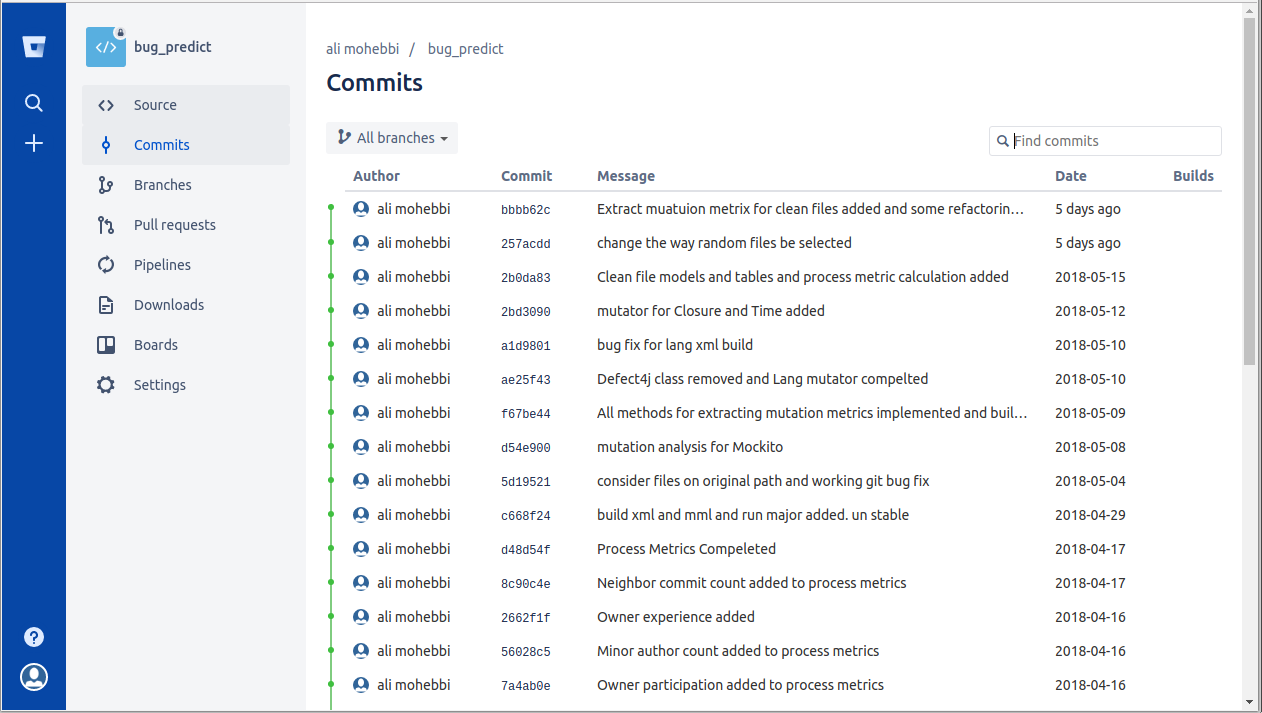
\includegraphics[width=1\textwidth]{img/case_study/bitbucket.png}
	\caption{نمایی از مخزن نرم‌افزاری}
	\label{fig:bitbucket}
\end{figure}



\section{رویکرد اول : معیارهای فرآیند در کنار جهش}
در این قسمت  چگونگی استخراج معیارهای رویکرد اول شرح داده می‌شود. ابتدا لازم است اطلاعات مربوط به ثبت‌های  حاوی خطا از ابزار \lr{defects4j} بازیابی شود و سپس این اطلاعات با استفاده از مخرن نرم‌افزاری تکمیل شود. در مراحل بعد ابتدا معیار‌های فرآیند و سپس معیارهای جهش استخراج خواهند شد. 

\subsection{ استخراج اطلاعات مربوط به ثبت‌های   حاوی خطا}
اطلاعاتی که درباره‌ی ثبت‌های حاوی خطا قابل بازیابی است در زیر آمده است:
\begin{enumerate}
\item شناسه‌ی ثبت در مخزن 
\item نام فایل حاوی خطا
\item شماره ی خطا در ابزار \lr{defects4j}
\item شماره‌ی ثبت تعمیر خطا
\item نام پروژه
\item نام انتشار قبلی پروژه
\item شماره‌ی ثبت انتشار قبلی پروژه
\end{enumerate}

از میان اطلاعات بالا همگی به سادگی با استفاده از ابزار defect4j قابل استخراج است بجز دو مورد آخر. همچنین شماره‌ی ثبت تعمیر مورد استفاده قرار نگرفت ولی نگهداری شد چراکه ممکن بود لازم شود. 
برای بدست آوردن اطلاعات مربوط به هر انتشار لازم است که مخرن نرم افزاری هر پروژه مورد بررسی قرار گیرد. در  مخازن پروژه‌های نرم‌افزاری  از نوع گیت برای مشخص کردن یک رویداد مهم از \نام{تگ}{Tag} استفاده می‌شود. هر تگ می‌تواند به یک ثبت از برنامه اشاره کند. تگ می‌تواند نمایانگر رویدادهایی چون انتشار برنامه، انتشار بتا، و یا کاندید انتشار باشد. بنابرین با استفاده از تگ می‌تواند انتشار را پیدا کرد.\\

تگ‌های مخازن گیت دو نوع \واژه{سبک‌وزن} و \واژه{حاشیه‌نویسی شده} که در میان پروژه‌های مورد مطالعه از هر دو نوع جهت مشخص کردن انتشار استفاده شده است.  کار کردن با این دو نوع تگ دارای تفاوتهایی در پیاده‌سازی است که در ایتجا از پرداختن به جزییات صرف نظر می‌شود. \\ ابتدا همه‌ی تگ‌های موجود در مخازن نرم‌افزاری استخراج می‌شود و در پایگاه داده قرار می‌گیرد. از میان تگ‌های استخراج شده تگ‌های نا مرتبط با انتشار از پایگاه داده حذف می‌شود. تگ‌های نامرتبط با توجه به نام آنها مشخص می‌شود به عنوان مثال تگ‌هایی که حاوی لغات Beta یا Dev هستند نامرتبط  محسوب می‌شوند. در نهایت جدولی به نام ReleaseProject ساخته می‌شود که در آن اطلاعات انتشارهای مختلف وجود دارد. نمایی از این جدول در شکل \ref{fig:project-release} آمده است. \\
\begin{figure}[H]
	\centering
	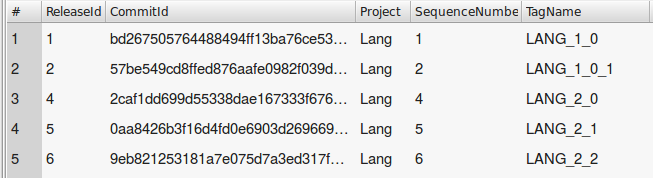
\includegraphics[width=1\textwidth]{img/case_study/project-release.png}
	\caption{نمایی از جدول محتوای انتشارها}
	\label{fig:project-release}
\end{figure}


در قدم بعدی باید مشخص شود اولین انتشار ما قبل هر ثبت حاوی خطا کدام است. برای این منظور لیست ثبت‌ها  در یک پروژه به ترتیب زمانی بررسی می‌شود. اولین ثبت  ماقبل ثبت مورد نظر که مربوط به یک انتشار است یافت می‌شود و به عنوان انتشار ماقبل آن ثبت در نظر گرفته می‌شود. \\

 در نهایت جدولی به نام BugInfo تولید شده که نمایی از آن در شکل \ref{fig:bug-info} آمده است. این جدول ۴۰۵ سطر دارد که بیشتر از تعداد کل خطاهای ذکر شده در مجموعه داده‌ی \lr{defects4j} است. علت این است که یک خطا می‌تواند خطا در چندین پرونده به طور همزمان باشد و از آنجا که پیش‌بینی در سطح پرونده انجام می‌شود لازم است اطلاعات برای پرونده‌ها ذخیره شود.

\begin{figure}[H]
\centering
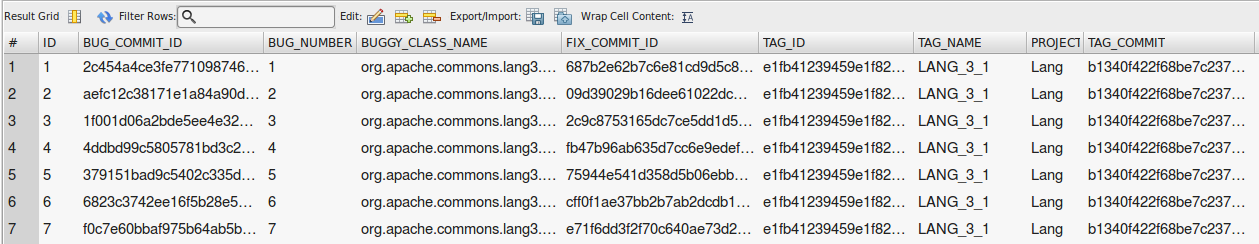
\includegraphics[width=1\textwidth]{img/case_study/bug-info.png}
\caption{نمایی از جدول محتوای اطلاعات پرونده‌های حاوی خطا}
\label{fig:bug-info}
\end{figure}

\subsection{انتخاب پرونده‌های سالم}
همانطور که مطرح شد تعداد پرونده‌های حاوی خطا برابر ۴۰۵ عدد است که از تعداد کل پرونده‌ها کمتر است. بنابرین جهت ساخت مدلهای بدون جهت‌گیری به همین تعداد پرونده‌های بدون خطا به طور تصادفی انتخاب می‌شود. بدین ترتیب یک مجموعه داده‌ی \واژه{متعادل} حاوی ۸۱۰ پرونده ساخته شده است. این روش طبق مقاله‌ی \cite{johannessen2008data} به کار گرفته شده است. در این انتخاب به تعداد پرونده‌های حاوی خطا، پرونده‌های بدون خطا انتخاب می شود. \\به ازای هر پرونده‌ی دارای خطا در همان ثبت از پروژه‌ی مربوط یک پرونده‌ی بدون خطا به صورت تصادفی انتخاب می‌شود. برای این کار لیست تمام پرونده‌های داخل پروژه در ثبت فایل حاوی خطا در نظر گرفته می‌شود و یک فایل به صورت تصادفی انتخاب می‌شود. این پرونده نباید جز پرونده‌های حاوی خطا در آن ثبت از  پروژه باشد.  البته ممکن اسن پرونده در ثبت‌های بعدی یا قبلی خطا داشته باشد و از این نظر محدودیتی ندارد. همانطور که گفته شد یک ثبت ممکن از بیش از یک فایل حاوی خطا داشته باشد. سپس مشخصات این فایل در جدول CleanInfo قرار می گیرد. نمایی از این جدول در تصویر \ref{fig:clean-info} آورده شده است.
\begin{figure}[H]
	\centering
	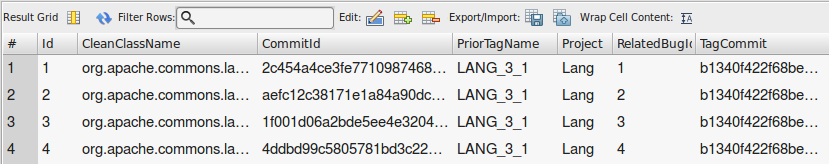
\includegraphics[width=1\textwidth]{img/case_study/clean-info.png}
	\caption{نمایی از جدول محتوای اطلاعات پرونده‌های سالم}
	\label{fig:clean-info}
\end{figure}



\subsection{ استخراج معیارهای فرآیند}
در  این قسمت نحوه‌ی استخراج هر یک از معیارهای ذکر شده در قسمت \ref{sec:method-phase1} بیان می‌شود. \\
\textbf{‫تعداد ثبت در سیستم کنترل نسخه‬:}
اولین راه حلی که به ذهن می‌رسد استفاده ی مستقیم از Jgit برای این کار است.  به این صورت که تعداد ثبت‌های بین ثبت کنونی و انتشار قبلی  بررسی کرده و تعداد  ثبت‌هایی که در آن‌ها فایل حاوی خطا تغییر کرده است شمرده شوند. مشکل این راه این است که بسیار پر هزینه  خواهد بود زیرا مرتبا باید عملیات \واژه{ورودی/خروجی} بر روی دیسک انجام پذیرد و همچنین بررسی‌های تکراری بسیاری انجام می‌گیرد. به عنوان مثال دو ثبت حاوی خطا را در نظر بگیرید که دارای انتشار ما قبل یکسانی هستند. تعدادی از بررسی‌های ثبت‌های ما بین آن‌ها تا ثبت مربوط به انتشار دارای همپوشانی خواهد بود. از طرف دیگر می‌توان اطلاعاتی که در بررسی ثبت‌ها بدست می‌آید در محاسبه‌ی معیارهای دیگر نیز مورد استفاده قرار گیرد.\\

همچنین برای یافتن ثبت‌های بین انتشار و ثبت مورد نظر نمی‌توان از تاریخ ثبت آنها استفاده کرد. زیرا تعداد زیادی از ثبت‌های ابتدای  برخی پروژه ‌های مورد مطالعه دارای تاریخ یکسانی هستند استفاده از تاریخ غیر ممکن می‌شود. علت داشتن تاریخ یکسان احتمالاً مهاجرت از یک نوع مخرن نرم‌افزاری به نوع گیت بوده است. \\

 بنابرین کل ثبت‌های پروژه‌ها مورد بررسی قرار گرفت و دو جدول تولید شد.
جدول اول به نام CommitInfo‌ که اطلاعات کلی ثبت‌ها را در بر می‌گیرد و جدول دوم  CommitChangedFile که اطلاعات مربوط به پرونده‌هایی که در یک ثبت از برنامه نسبت به ثبت قبلی تغییر کرده است نگهداری می‌شود.  در این جدول برای هر پرونده تعداد خطوط اضافه و کم شده نسبت به ثبت قبلی ذخیره شده است. در جدول اول \lr{Sequence\textunderscore Number} نشان می‌دهد که چندمین نسخه از ابتدای پروژه می‌باشد و این عدد در هنگام بررسی‌ها به آن ثبت داده‌ شده زیرا برای یافتن ثبت‌های بین ثبت کنونی و ثبت مربوط به انتشار قبلی لازم است از آنها استفاده شود. \\
  هر سطر از جدول دوم یک کلید خارجی دارد به سطری از جدول اول. قسمتی از جدول CommitInfo  در شکل \ref{fig:commit-info} و جدول CommitChangeFile در شکل \ref{fig:change-file-info}  زیر آمده است:

\begin{figure}[H]
	\centering
	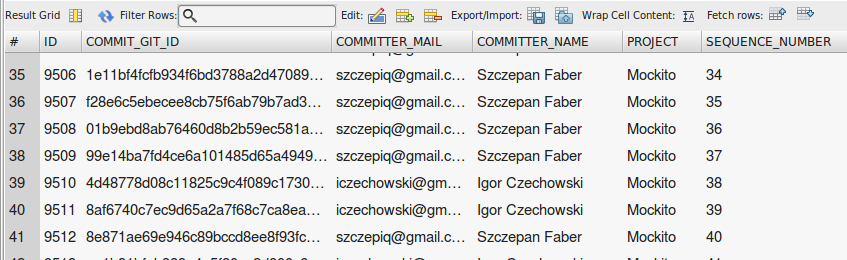
\includegraphics[width=1\textwidth]{img/case_study/commit-info.png}
	\caption{نمایی از جدول اطلاعات ثبت‌ها}
	\label{fig:commit-info}
\end{figure}


\begin{figure}[H]
	\centering
	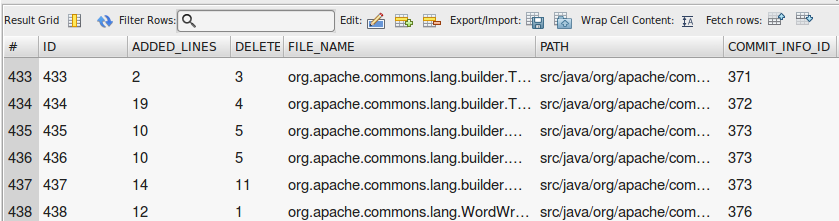
\includegraphics[width=1\textwidth]{img/case_study/change-file-info.png}
	\caption{ نمایی از جدول تغییرات پرونده‌ها در ثبت‌ها }
	\label{fig:change-file-info}
\end{figure}

در نهایت با استفاده از قطعه کد \ref{code:commit-info} اطلاعات مربوط به ثبت مورد نظر و ثبت انتشار بازیابی می‌شوند و سپس  از شماره‌ی دنباله‌ی آنها در پرسمان موجود در قطعه کد \ref{code:ncomm} استفاده می‌شود و معیار محاسبه می‌گردد.



\begin{latin}
	\begin{lstlisting}[language=SQL]
SELECT  * from CommitInfo CI where CI.COMMIT_GIT_ID = :gitId AND CI.PROJECT = :project
\end{lstlisting}
\end{latin}
\captionof{lstlisting}{بازیابی اطلاعات ثبت}
\label{code:commit-info}

\begin{latin}
\begin{lstlisting}[language=SQL]
SELECT  count(*) from CommitChangedFile CC where CC.COMMIT_INFO_ID IN
	(SELECT CI.ID from CommitInfo CI WHERE CI.SEQUENCE_NUMBER BETWEEN 
	 :startSeq AND :endSeq AND CI.PROJECT = :project)
AND CC.FILE_NAME = :fileName
\end{lstlisting}
\end{latin}
\captionof{lstlisting}{محاسبه‌ی معیار تعداد ثبت‌ در سیستم کنترل نسخه}
\label{code:comm}

\متن‌سیاه{‫تعداد توسعه‌دهندگان فعال:‬}
به منظور محاسبه‌ی این معیار تعداد آدرس ایمیل‌های ثبت‌کننده‌های ثبت‌هایی شمرده می‌شود که آن ثبت‌ها شماره‌ی دنباله‌ی آنها بین شماره‌ی دنباله‌ی ثبت پرونده‌ی مورد نظر و ثبت انتشار قبلی است و همچنین در آن ثبت پرونده‌ی مورد نظر در آن ثبت‌ها تغییر کرده است. به عبارت دیگر ثبت‌هایی که نام پرونده در جدول  CommitChangeFile  برای آن‌ها وجود دارد. 

\begin{latin}
\begin{lstlisting}[language=SQL]
SELECT  count(DISTINCT CI.COMMITTER_MAIL) from CommitInfo CI WHERE
CI.SEQUENCE_NUMBER BETWEEN :startSeq AND :endSeq AND CI.PROJECT = 
project AND CI.ID IN 
	(SELECT CC.COMMIT_INFO_ID from CommitChangedFile CC where CC.FILE_NAME = :fileName)
\end{lstlisting}
\end{latin}
\captionof{lstlisting}{محاسبه‌ی تعداد توسعه‌دهندگان فعال}

\textbf{تعداد توسعه‌دهندگان متمایز:}
برای محاسبه‌ی معیار از پرسمان قبلی استفاده می‌شود اما اینبار به جای استفاده \lr{Sequence\_Number} انتشار قبلی، عدد یک  قرار داده می‌شود که از ابتدای پروژه توسعه دهندگان شمرده شوند. 
\\

\متن‌سیاه{‫مقدار نرمال‌سازی شده‌ی تعداد خطوط اضافه شده:‬}
از پرسمان \ref{code:added-line-file} جهت محاسبه‌ی مجموع تعداد خطوط اضافه شده به پرونده در طول انتشار استفاده می‌شود و از پرسمان \ref{code:added-line-project} جهت محاسبه‌ی مجموع خطوط اضافه شده به پروژه استفاده می‌شود. سرانجام حاصل پرسمان اول بر دوم تقسیم می‌شود. 

\begin{latin}
	\begin{lstlisting}[language=SQL]
SELECT sum(CC.ADDED_LINES) from CommitChangedFile CC where
CC.COMMIT_INFO_ID IN
	(SELECT CI.ID from CommitInfo CI WHERE CI.SEQUENCE_NUMBER BETWEEN 
	:startSeq AND :endSeq AND CI.PROJECT = :project)
AND CC.FILE_NAME = :fileName
	\end{lstlisting}
\end{latin}
\captionof{lstlisting}{محاسبه‌ی تعداد خطوط اضافه شده به پرونده}
\label{code:added-line-file}

\begin{latin}
\begin{lstlisting}[language=SQL]
SELECT  sum(CC.ADDED_LINES) from CommitChangedFile CC where 
CC.COMMIT_INFO_ID IN
	(SELECT CI.ID from CommitInfo CI WHERE CI.SEQUENCE_NUMBER
	 BETWEEN :startSeq AND :endSeq AND CI.PROJECT = :project)
\end{lstlisting}
\end{latin}
\captionof{lstlisting}{محاسبه‌ی تعداد خطوط اضافه شده به پروژه}
\label{code:added-line-project}

\متن‌سیاه{‫مقدار نرمال‌سازی شده‌ی تعداد خطوط حذف شده:‬} به طور مشابه معیار قبلی محاسبه می‌گردد.

\textbf{درصد خطوطی که مالک فایل مشارکت کرده:}
دستور Blame در Jgit نشان می‌دهد که هر خط از پرونده در یک ثبت  در کدام یک از ثبت‌های گذشته اضافه شده است.  با یافتن ثبت مسئول اضافه کردن آن خط نویسنده‌ی آن خط مشخص می‌شود که همان ثبت‌کننده است. با کمک این دستور به دلایل مشابه ساخت جداول مربوط به ثبت‌ها، جدولی با عنوان Participation ساخته شده که در آن هر سطر نشان می‌دهد که یک نویسنده در یک نسخه از برنامه چند درصد از خطوط به وی اختصاص دارد. در شکل \ref{fig:participation} نمایی از این جدول آورده شده است.  از این جدول علاوه بر محاسبه‌ی این معیار برای یافت سایر معیارها نیز استفاده خواهد شد. در نهایت معیاری که در ابتدا بسیار پیچیده به نظر می رسید به کمک پرسمان ساده‌ی \ref{code:own} محاسبه خواهد شد. 

\begin{figure}[H]
	\centering
	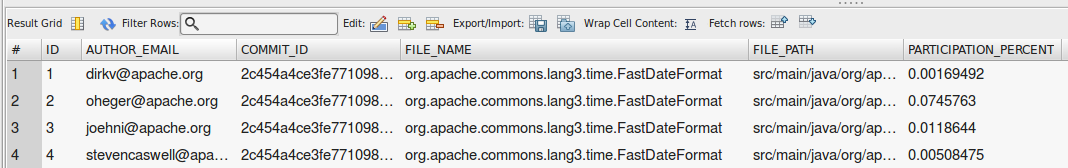
\includegraphics[width=1\textwidth]{img/case_study/participation.png}
	\caption{نمایی از جدول مشارکت‌کنندگان در ویرایش پرونده‌ها}
	\label{fig:participation}
\end{figure}


\begin{latin}
	\begin{lstlisting}[language=SQL]
SELECT max(PARTICIPATION_PERCENT) from Participation P 
where COMMIT_ID = :commitId AND FILE_NAME = :fileName")
\end{lstlisting}
\end{latin}
\captionof{lstlisting}{محاسبه‌ی درصد خطوط مالک پرونده}
\label{code:own}

\textbf{تعداد مشارکت‌کنندگان جزئی:‬}
 با استفاده از جدول Participation و پرسمان  \ref{code:minor}  معیار محاسبه می‌شود. مقدار minorThereshold برابر ۵ درصد قرار می‌گیرد.

\begin{latin}
	\begin{lstlisting}[language=SQL]
SELECT count(AUTHOR_EMAIL) from Participation P 
where COMMIT_ID = :commitId AND FILE_NAME = :fileName
and PARTICIPATION_PERCENT < :minorThreshold
\end{lstlisting}
\end{latin}
\captionof{lstlisting}{محاسبه‌ی تعداد مشارکت‌کنندگان جزئی}
\label{code:minor}

\textbf{تعداد ثبت‌های همسایگان:‬}
ابتدا لازم است که همسایگان پرونده در یک ثبت و نیز تعداد دفعات همسایگی در طول انتشار مشخص شود. این عمل به وسیله‌ی پرسمان \ref{code:neighbor} انجام می‌شود. سپس معیار تعداد ثبت‌ها در سیستم کنترل نسخه مشابه قبل با استفاده از کد \ref{code:comm} محاسبه می‌گردد و از آنها میانگین وزن‌دهی شده گرفته می‌شود.

\begin{latin}
\begin{lstlisting}[language=SQL]
SELECT FILE_NAME as `name`, count(ID) as `frequency` FROM
CommitChangedFile WHERE COMMIT_INFO_ID IN
	(SELECT COMMIT_INFO_ID FROM CommitChangedFile WHERE FILE_NAME = :fileName) 
AND COMMIT_INFO_ID IN
	(SELECT CI.ID from CommitInfo CI WHERE CI.SEQUENCE_NUMBER BETWEEN :startSeq AND :endSeq AND PROJECT = :project)
AND FILE_NAME != :fileName GROUP BY FILE_NAME
\end{lstlisting}
\end{latin}
\captionof{lstlisting}{یافتن همسایگان و تعدد همسایگی}
\label{code:neighbor}

\textbf{تعداد توسعه‌دهندگان فعال همسایگان:‬}
 به طور مشابه با معیار قبلی محاسبه می‌شود.\\
\textbf{‫تعداد توسعه‌دهندگان متمایز همسایگان:‬}
 به طور مشابه با معیار قبلی محاسبه می‌شود. \\

\textbf{تجربه‌ی مالک فایل:‬‬}
 برای محاسبه‌ی معیار ابتدا   با استفاده از پرسمان \ref{code:find-owner} مالک پرونده مشخص می‌شود. سپس تعداد ثبت‌هایی که مالک پرونده از ابتدای پروژه تا آن زمان ثبت کرده است  با استفاده از پرسمان \ref{code:commit-of-commiter} شمرده می‌شود. به ترتیب از دو جدول Participation 
 و 
 CommitInfo  استفاده می‌شود.

\begin{latin}
\begin{lstlisting}[language=SQL]
SELECT AUTHOR_EMAIL FROM Participation P WHERE COMMIT_ID = :commitId 
AND FILE_NAME = :fileName AND PARTICIPATION_PERCENT  = 
	(SELECT max(PARTICIPATION_PERCENT) FROM Participation P2 
	 WHERE P2.COMMIT_ID = :commitId  AND P2.FILE_NAME = :fileName)
\end{lstlisting}
\end{latin}
\captionof{lstlisting}{یافتن مالک پرونده}
\label{code:find-owner}



\begin{latin}
\begin{lstlisting}[language=SQL]
SELECT  count(*) from CommitInfo CI where CI.SEQUENCE_NUMBER BETWEEN
:startSeq AND :endSeq AND CI.PROJECT = :project AND CI.COMMITTER_MAIL =
:authorEmail
\end{lstlisting}
\end{latin}
\captionof{lstlisting}{شمارش تعداد ثبت‌های یک ثبت کننده در بازه‌ی زمانی داده شده}
\label{code:commit-of-commiter}

\textbf{‫تجربه‌ی تمام مشارکت‌کنندگان:‬}
ابتدا همه‌ی توسعه‌دهندگان پرونده با استفاده از پرسمان \ref{code:contributers} مشخص می‌شوند.  سپس میزان تجربه‌ی هر یک با استفاده از پرسمان \ref{code:commit-of-commiter} جداگانه محاسبه می‌شود و از آن‌ها میانگین هندسی گرفته می شود. 
\begin{latin}
\begin{lstlisting}[language=SQL]
SELECT AUTHOR_EMAIL FROM Participation P WHERE COMMIT_ID = :commitId 
AND FILE_NAME = :fileName
\end{lstlisting}
\end{latin}
\captionof{lstlisting}{یافتن مشارکت‌کنندگان در پرونده}
\label{code:contributers}


در نهایت جدولی برای معیارهای فرآیند تولید می‌شود که نمایی از آن در شکل \ref{fig:process-metics} آورده شده است. 
\begin{figure}[H]
	\centering
	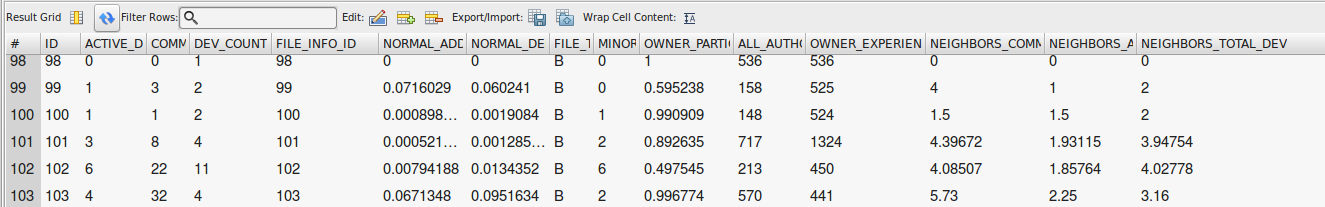
\includegraphics[width=1\textwidth]{img/case_study/process-metrics.png}
	\caption{نمایی از جدول معیارهای فرآیند }
	\label{fig:process-metics}
\end{figure}


\subsection{استخراج معیارهای جهش}
روند کلی به این صورت است که برای هر سطر از جدول BugInfo   یا CleanInfo که معادل یک  پرونده  در یک نسخه است ابتدا آن نسخه از برنامه در پوشه‌ی کاری قرار می‌گیرد. منظور از پوشه‌ی کاری محلی است  که پرونده‌های پروژه از مخزن نرم‌افزاری فراخوانی می‌شود و در آن قرار می گیرد. سپس به فایل build.xml    و یا build.gradle  قطعه کدهایی  به منظور  اجرای  صحیح فرآیند ساخت اضافه می‌شود.  \\
همچنین جهت تولید جهش‌یافته و تحلیل جهش لازم است برای هر پروژه پیکربندی‌هایی انجام شود که این پیکربندی‌ها با اجرای عملیات مهندسی معکوس در ابزار \lr{Defects4j} به دست آمد. به منظور انجام مهندسی معکوس کدهای ابزار که به زبان \نام{پرل}{Perl} نوشته شده‌اند مورد بررسی قرار گرفتند و نحوه‌ی عملکرد ابزار با پروژه‌های مختلف و پیکربندی‌ها مشخص شد. \\
از آنجا که اجرای تحلیل جهش زمان زیادی می‌گیرد برای انجام آن یک رایانه به صورت اختصاصی برای انجام آن در \نام{ آزمایشگاه کیفیت نرم‌افزار}{Software Quality Research Lab - \url{http://sqrlab.ce.sharif.edu/}} واقع در دانشگاه صنعتی شریف در نظر گرفته شد. این رایانه به یک سرور \نام{لینوکس}{Linux} تبدیل شد تا امکان نظارت و رفع خطا در استخراج معیارهای جهش همواره امکان پذیر باشد و استخراج معیارها و توسعه‌ی سایر قسمت‌های این پژوهش به صورت موازی انجام گیرد. جزییات تبدیل رایانه به سرور لینوکس در پیوست آمده است. \\
از آنجا که انجام تحلیل جهش بر روی موارد مطالعاتی صنعتی انجام گرفته است و پروژه‌های انتخاب شده حجم زیادی دارند لازم است تا پیکربندی‌هایی در نظر گرفته شود تا از بروز خطا و توقف محاسبات جلوگیری شود. این پیکربندی‌ها در زیر آمده است.  
\begin{itemize}
	 \setlength{\itemsep}{1pt}
	\setlength{\parskip}{0pt}
	\setlength{\parsep}{0pt}

\item 
\متن‌سیاه{افزایش فضای \نام{PermGen}{Premanent Generation}:}  
این فضا  یک \نام{هیپ}{Heap} مخصوص است که از فضای هیپ اصلی جاوا مجزا است و در آن \واژه{ماشین مجازی جاوا} \واژه[فراداده‌های]{فراداده} کلاس‌های بارگذاری شده را ردگیری می‌کند. به دلیل حجم زیاد پروژه‌های مورد مطالعه لازم است که این فضا بیشتر از حالت پیش‌فرض قرار داده شود. برای انجام این پژوهش فضای ۲ گیگابایت در نظر گرفته شده است. 
\item
\متن‌سیاه{افزایش فضای Codecache :} 
کدهای ترجمه شده به زبان ماشین در این فضا قرار می‌گیرد که به دلیل مشابه پیکربندی قبلی لازم است این فضا از حالت پیش‌فرض بیشتر باشد. فضای در نظر گرفته شده ۵۱۲ مگابایت می‌باشد. 
\item
\متن‌سیاه{قرار دادن \واژه{زمان خروج} :}
زمانی که یک جهش یافته از کد اصلی ساخته می‌شود ممکن است که جریان کنترلی به نحوی تغییر کند که برنامه در حلقه‌ی بی‌نهایت یا بن‌بست قرار گیرد. برای جلوگیری از چنین حالتی لازم است تا در تنظیمات ابزار JUnit  مهلت زمانی در نظر گرفته شود تا در صورت قرارگیری در چنین شرایطی پس از مدت زمان معین اجرای مورد آزمون متوقف شود و مورد آزمون شکست خورده تلقی شود. مدت زمان تعیین شده جهت خروج ۱۳ ثانیه می‌باشد. 
\متن‌سیاه{عملگرهای جهش انتخابی}
با توجه به هزینه‌ی زمانی تحلیل جهش به کارگیری تمامی عملگرهای موجود در ابزار Major به صرفه نمی‌باشد. برای تولید جهش‌یافته‌ها از مجموعه عملگرهای استفاده شده در مقاله‌ی بوئز و همکاران\cite{bowes2016mutation} استفاده شده که مطابق عملگرهای پیش‌فرض در ابزار   PIT‌ می‌باشد. پرونده‌ی MML ساخته شده در شکل \ref{fig:mml-used}

\begin{figure}[H]
	\centering
	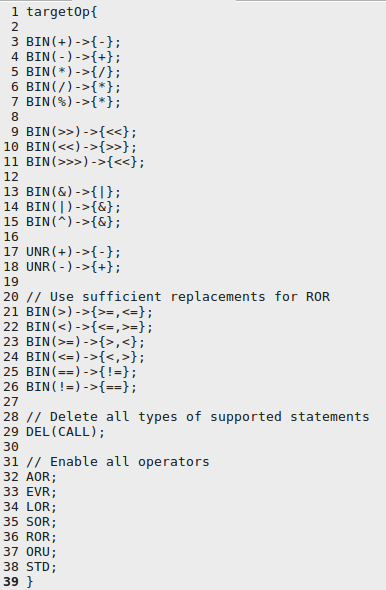
\includegraphics[width=.7\textwidth]{img/case_study/mml-used.png}
	\caption{پرونده‌ی mml ساخته شده جهت تولید جهش‌یافته‌ها}
	\label{fig:mml-used}
\end{figure}
\end{itemize}
 پس از انجام تحلیل جهش برای پرونده‌های حاوی خطا و سالم نتایج در جدول MutationMetrics قرار داده شد که نمایی از این جدول در شکل \ref{fig:mutation-metrics}  آمده است. 
 
 
 \begin{figure}[H]
 	\centering
 	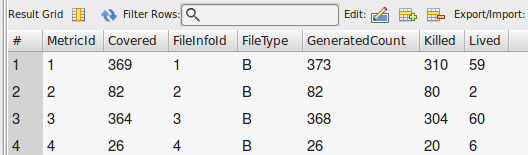
\includegraphics[width=.7\textwidth]{img/case_study/mutation-metrics.png}
 	\caption{نمایی از جدول نتایج تحلیل جهش}
 	\label{fig:mutation-metrics}
 \end{figure}
 
\subsection{ معیارهای فرآیند مبتنی بر جهش}
همانطور که در قسمت \ref{sec:method-phase-two} اشاره شده چهار معیار معرفی شدند و مبتنی بر جهش نامیده شدند. این قسمت به نحوه‌ی پیاده‌سازی دسته‌ی دوم از معیارها را شرح خواهد داد. 
\begin{itemize}
\item
\متن‌سیاه{تعداد جهش‌یافته‌های تولید شده‌ی جدید نسبت به انتشار قبلی برنامه:}
به منظور محاسبه‌ی این معیار ابتدا لازم است که مشخص شود که پرونده‌ی مورد نظر نسبت به انتشار قبلی چه تغییراتی داشته است. این کار با استفاده از ابزار JGit انجام  می‌شود. JGit این امکان را فراهم می‌کند که دو پرونده در دو ثبت متفاوت مقایسه شوند و مشخص می‌کند که کدام خطوط حذف شده‌اند و کدام خطوط اضافه شده‌اند. در اینجا لازم است خطوط اضافه شده  مشخص شود. سپس با استفاده از ابزار Major جهش‌یافته‌ها تولید می‌شود. در  قسمت  \ref{sec:tools-major} توضیح داده شد که پس تولید جهش‌یافته‌ها یک فایل خروجی نیز به نام mutant.log تولید می‌شود که در آن مشخص شده در هر خط از برنامه چه جهش‌یافته‌هایی تولید شده است. حال کافیست تعداد جهش‌یافته‌های تولید شده در خطوطی شمرده شوند که ابزار Jgit آن‌ها را به عنوان خطوط جدید نسبت به انتشار قبلی معرفی کرده است. بدین ترتیب این معیار محاسبه خواهد شد.\\
لازم به ذکر است روش یاد شده پایه‌ی محاسبه‌ی معیار بعدی و معیارهای رویکرد سوم است.
\item
\متن‌سیاه{تعداد جهش‌یافته‌های متمایز در چند انتشار اخیر:}

 به منظور افزایش کارایی ابتدا بررسی می‌شود که فایل مورد نظر در آن انتشار وجود دارد یا خیر در صورت عدم وجود محاسبات برای آن انتشار انجام نمی‌گیرد.
برای محاسبه ابتدا چهار انتشار قبلی  با استفاده از پرسمان  پرسمان مناسب از جدول ProjectRelease بازیابی می‌شود. سپس مشابه معیار قبلی جهش‌یافته‌های جدید نسبت به انتشار قبلی برای هر انتشار محاسبه می‌شود و با هم جمع زده می‌شود.  یک جدول برای نتایج تولید جهش‌یافته‌ها  به نام  DistinctMutantLog در نظر گرفته شده که تعداد جهش‌یافته‌های جدید برای هر انتشار نسبت به انتشار قبلی در آن ذخیره می‌گردد. از مزایای ایجاد این جدول پایداری در انجام محاسبات است به عنوان مثال  در صورت توقف محاسبات امکان از سرگیری محاسبات از محل توقف وجود  دارد و همچنین  با نگهداری به عنوان یک مجموعه داده می‌تواند در پژوهش‌های دیگر به کار گرفته شود. نمایی از جدول در شکل زیر آمده است. به طور مثال سطر اول جدول بیان می‌کند که در انتشاری از برنامه با شماره ثبت  \lr{..21a}  پرونده‌ی شماره یک شماره یک از فایلهای حاوی خطا 430 جهش‌یافته‌ی جدید نسبت به انتشار قبلی داشته است.
\begin{comment}
\begin{latin}
	\begin{lstlisting}[language=SQL]
SELECT * FROM ProjectRelease WHERE Project = :project AND
 SequenceNumber <  
	(SELECT SequenceNumber FROM ProjectRelease WHERE 
	 Project = :project AND CommitId = :releaseCommit) 
 ORDER BY SequenceNumber DESC LIMIT 4 
\end{lstlisting}
\end{latin}
\captionof{lstlisting}{بازیابی چهار نسخه‌ی اخیر یک ثبت}
\label{code:previous-releases}
\end{comment}

\begin{figure}[H]
	\centering
	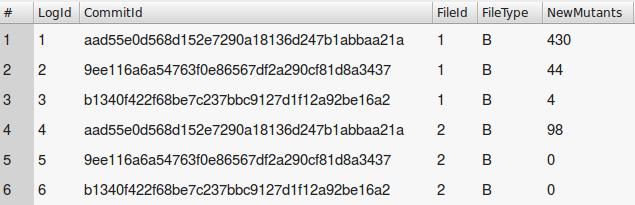
\includegraphics[width=1\textwidth]{img/case_study/distinct-mutant-log.png}
	\caption{نمایی از جدول تعداد جهش‌یافته‌های متمایز در انتشارها}
	\label{fig:distinct-mutant-log}
\end{figure}
\item
\متن‌سیاه{میزان تغییرات مثبت امتیاز جهش  در چند انتشار اخیر:}
ابتدا انتشارها  مشابه معیار قبلی بازیابی می‌شوند و سپس برای هر یک تحلیل جهش انجام می‌گردد. نتایج جهش در جدولی به نام ReleaseMutation قرار می‌گیرد.  نمایی از این جدول در شکل  \ref{fig:release-mutation} آمده است. سپس هر انتشار با انتشار قبلی مقایسه می‌شود و در صورتی که تغییر امتیاز جهش  مثبت باشد با مجموعه تغییرات مثبت جمع می‌گردد. 
\begin{figure}[H]
	\centering
	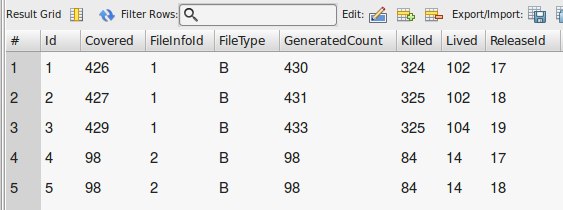
\includegraphics[width=1\textwidth]{img/case_study/release-mutation.png}
	\caption{نمایی از جدول نتایج تحلیل جهش در انتشارها}
	\label{fig:release-mutation}
\end{figure}
\item
\متن‌سیاه{میزان تغییرات منفی امتیاز جهش  در چند انتشار اخیر:}
به طور مشابه با معیار قبلی عمل می‌گردد با این تفاوت که تغییرات منفی در نظر گرفته می‌شود. 
\end{itemize}

\subsection{معیارهای ترکیبی جهش-فرآیند}

نحوه‌ی محاسبه به این صورت خواهید بود که ابتدا ثبت‌هایی از برنامه در طول آخرین انتشار که در آن فایل مورد نظر تغییر کرده است  توسط  پرسمان   مناسب بازیابی می شود. سپس برای هر ثبت تعداد جهش یافته‌های جدید نسبت به ثبت قبلی محاسبه می‌شود و برای محاسبه‌ی جهش‌یافته‌های حذف شده تعداد جهش یافته‌ها در  ثبت قبلی را یافته و آن‌ها که جز خطوط حذف شده در ثبت بعدی است شمرده می شود. تعداد جهش‌یافته‌های اضافه و حذف شده در ثبت‌ها جمع شده و بر تعداد ثبت‌های کل پروژه در طول انتشار تقسیم می گردد.

\begin{comment}

\begin{latin}
\begin{lstlisting}[language=SQL]
SELECT CC.* from CommitChangedFile CC, CommitInfo CI where CC.COMMIT_INFO_ID = CI.ID
AND CI.SEQUENCE_NUMBER BETWEEN :startSeq AND :endSeq
AND CI.PROJECT = :project
AND CC.FILE_NAME = :fileName ORDER BY CI.SEQUENCE_NUMBER asc
\end{lstlisting}
\end{latin}
\captionof{lstlisting}{بازیابی اطلاعات ثبت‌هایی که یک فایل در بازه‌ی مشخص در آنها تغییر کرده است}
\label{code:commit-during-release}
\end{comment}
\chapter{ارزیابی}
\label{chap:evaluation}
در این بخش به تشریح نحوه‌ی ساخت مدل‌های پیش‌بینی و ارزیابی معیارهای شرح داده شده در فصل \ref{chap:method} پرداخته می‌شود. با استفاده از معیارهای استخراج شده در فصل \ref{chap:case-study} مدل‌های مورد نظر ساخته می‌شوند. ساخت مدل‌ها در زبان R و به وسیله‌ی بسته‌ی \نام{کرت}{Caret} \cite{kuhn2008caret} انجام می‌شود.\\
در ابتدا ۱۰ درصد از داده‌ها به عنوان داده‌ی آزمون جدا می‌شود. با استفاده از ۹۰ درصد باقی‌مانده به ساخت مدل پرداخته می‌شود. در ساخت و ارزیابی مدل‌ها از روش \واژه{اعتبارسنجی متقابل} استفاده می‌شود که تعداد دسته‌ها ۱۰ و تعداد تکرار نیز ۱۰ بار می‌باشد. لازم به ذکر است که دسته‌بندی‌ها به طور تصادفی انجام می‌شود.  همچنین در بسته‌ی کرت در هر روش دسته‌بندی پارامترهای مختلفی به طور پیش فرض به کار گرفته می‌شود تا بهترین مدل ممکن ساخته شود.  با استفاده از  اعتبارسنجی متقابل و تنظیم خودکار پارامترهای مختلف مدل نهایی ساخته شده و از این مدل برای پیش‌بینی داده‌های آزمون  استفاده شده است.  \\
در این ارزیابی از  روش‌های دسته‌بندی \واژه{درخت تصمیم}، \واژه{ماشین بردار پشتیبانی}، \واژه{رگرسیون منطقی} و \واژه{شبکه‌ی عصبی} استفاده شده است. این روش‌های دسته‌بندی بیش از سایرین در مقالات مورد استفاده قرار گرفته‌اند. در ادامه هر یک از رویکردها به طور جداگانه ارزیابی شده و نتایج در زیر آمده است. 


\section{ارزیابی معیارهای فرآیند و جهش}
همانطور که اشاره شد هدف از این آزمایش این است که مشخص شود قرارگیری معیارهای جهش در کنار معیارهای فرآیند باعث بهبود پیش‌بینی خطا می‌گردد یا خیر و این تاثیر تا چه میزان است. به همین منظور  با استفاده از ۱۲ معیار فرآیند یک مدل پیش‌بینی ساخته شده و مدل دیگری  با استفاده از ۱۲ معیار فرآیند و ۴ معیار جهش ساخته شده است.  معیارهای فرآیند  و جهش مورد استفاده از پژوهش‌های گذشته انتخاب شده‌اند که در قسمت‌های \ref{subsec:metrics} و \ref{sec:mutation} معرفی شدند. 
در نهایت این دو مدل با استفاده از معیارهای ارزیابی مختلف با هم مقایسه شده‌اند. بدیهی است که دو مدلی که با هم مقایسه می‌شوند به جز در معیارهای استفاده شده (بردار ویژگی) به منظور ساخت مدل از هیچ منظری تفاوت ندارند و داده‌های  پرونده‌های یکسانی در ساخت و ارزیابی آنها استفاده شده. پارامترهای استفاده شده در مدلهای ساخته شده جدول \ref{tab:param1} آمده است.\\

 \begin{table}[H] 
	\renewcommand*{\arraystretch}{1.3}	
	\centering \caption{پارامترهای مدل ساخته شده}
	\label{tab:param1}
	\begin{tabular}{|c|c|c|}
		\hline
شماره مدل&نام روش & پارامتر \\
		\hline
		\hline
		1	& DT & \lr{cp = 0.125}\\
		\hline
		 1	& SVM & \lr{kernel = polynomial, degree =3, scale=0.1, cost=1}
		\\
		\hline
		1	& LR & - \\
		\hline
		1	& NN & \lr{hidden layers = 3, decay=0.1} \\
		\hline
			2	& DT & \lr{cp = 0.156}\\
		\hline
		2	& SVM & \lr{kernel = polynomial, degree =2, scale=0.1, cost=1}
		\\
		\hline
		2	& LR & - \\
		\hline
		2	& NN & \lr{hidden layers = 3, decay=0.1} \\
		\hline
		
	\end{tabular}
\end{table}

در جدول \ref{tab:eval-phase1} بخشی از نتایج آمده است. این نتایج نشان می‌دهد که قرار گیری معیارهای جهش در کنار معیارهای فرآیند موجب بهبود پیش‌بینی خطا به مقدار قابل ملاحظه‌ای می‌شود و در تمام  روش‌های  یادگیری موجب بهبود  پیش‌بینی می‌گردد. از میان روش‌های دسته‌بندی بهترین عملکرد   پس از افرودن معیارهای جهش  از نظر صحت و دقت را روش شبکه‌ی عصبی داشته است. همانطور  که در \ref{subsec:eval} توضیح داده شد  افزایش صحت به این معنی است که تعداد پیش‌بینی‌های صحیح بیشتر شده است. افزایش دقت نیز به این معنا است که نسبت داده‌هایی که به درستی خطادار پیش‌بینی شده‌اند  به کل داده‌هایی که به عنوان خطادار پیش‌بینی شده‌اند افزایش داشته است. روش   درخت تصمیم نیز بهترین عملکرد از نظر  معیار بازخوانی را  داشته است.  افزایش بازخوانی به این معنی است از بین داده‌های که خطادار بوده‌اند تعداد بیشتری در پیش‌بینی نیز خطادار مشخص شده‌اند. همچنین بیشترین تغییر مثبت در صحت پیش‌بینی پس از افزودن معیارهای جهش را روش شبکه‌ی عصبی   و  درخت تصمیم با مقدار $20$ درصد داشته است.  کمترین تاثیر با مقدار $7.5$ درصد در روش ماشین بردار پشتیبانی بوده است. بیشترین افزایش دقت در روش درخت تصمیم بوده است که مقدار آن $15.1$ درصد می‌باشد. از نظر معیار بازخوانی بیشترین تغییر مثبت را درخت تصمیم دارد که رشد $25$ درصدی داشته و روش رگرسیون منطقی کاهش $2.5$ درصدی داشته است. به طور کلی می‌توان این نتیجه را برداشت کرد که بیشترین بهبود در روش درخت تصمیم و کمترین در ماشین بردار پشتیبانی روی داده است.

 \begin{table}[H] 
	\renewcommand*{\arraystretch}{1.3}	
	\centering \caption{مقایسه‌ی معیارهای فرآیند و معیارهای 
		ترکیبی جهش-فرآیند}
	\rowcolors{4}{blue!15}{white}  
	\label{tab:eval-phase1}
	
	\begin{tabular}{|c|C{1cm}|C{1cm}|C{1.2cm}|C{1cm}|C{1cm}|C{1.2cm}|C{1cm}|C{1cm}|C{1.2cm}|}
		
		\hline
		\hline
		\multirow{2}{*}{نام روش} &
		\multicolumn{3}{c|}{صحت} &
		\multicolumn{3}{c|}{دقت} &
		\multicolumn{3}{c|}{بازخوانی} \\
		\cline{2-10}
		&	P & \lr{PM} & Diff & P & \lr{PM} & Diff & P & \lr{PM} & Diff\\
		\hline
		\hline
		
		DT &$0.587$&$0.787$&$+0.200$
		&$0.574$&$0.725$&$+0.151$&
		$0.675$&$0.925$&$+0.250$\\
		\hline
		SVM &$0.662$&$0.737$&$+0.075$&
		$0.685$&$0.806$&$+0.121$&
		$0.600$&$0.625$&$+0.025$\\		
		
		\hline
		LR &$0.612$&$0.725$&$+0.113$
		&$0.591$	&$0.736$&	$+0.145$
		&$0.725$&$0.700$&$-0.025$
		\\
		\hline
		NN‌&$0.612$&	$0.812$&	$+0.200$
		&$0.725$	&$0.777$	&$+0.052$
		&$0.591$	&$0.875$&	$+0.284$
		\\
		\hline
		
	\end{tabular}
\end{table}
\begin{comment}
\begin{table}[H] 
	\renewcommand*{\arraystretch}{1.3}	
	\centering \caption{مقایسه‌ی معیارهای فرآیند به تنهایی  و به همراه جهش}
	\label{tab:eval-phase1-old}
 \rowcolors{2}{blue!15}{white}   
	\begin{tabular}{|c|c|c|c|c|}
		
		\hline
		\hline
معیار & نام روش  & صحت & دقت & بازخوانی	
		\\
		\hline
		\hline
فرآیند & 
\lr{Decition Tree} & $0.587$&$0.574$&$0.675$
 \\
		\hline
		فرآیند و جهش & 
\lr{Decition Tree} & $0.787$&$0.725$&$0.925$
		\\
		\hline
فرآیند & 
\lr{SVM} & $0.662$&$0.685$&$0.600$
\\
\hline
فرآیند و جهش & 
\lr{SVM} & $0.737$&$0.806$&$0.625$
\\

\hline
فرآیند &
\lr{Logestic Regression} &   $0.612$&$0.591$&$0.725$
\\
\hline
فرآیند و جهش & 
\lr{Logestic Regression} & $0.725 $&$0.736$&$0.700$
\\
\hline
فرآیند &
\lr{Nueral Network} & $0.612$&$0.725$&$0.591$
\\
\hline
فرآیند و جهش & 
\lr{Nueral Network} & $0.812$&$0.777$&$0.875$
\\
\hline		
	\end{tabular}
\end{table}
\end{comment}
در شکل \ref{fig:ROC-phase1} نمودارهای ROC به تفکیک روش دسته‌بندی آمده است. در هر یک از زیر شکل‌ها منحنی ROC مربوط به  دو مدل با هم مقایسه شده است. درمدل اول که در ساخت آن از معیارهای فرآیند استفاده شده  با خط ممتد نمایش داده شده است و مدل دوم  از معیارهای فرآیند به همراه معیارهای جهش ساخته شده‌ است  و با خط‌چین نمایش داده شده‌. همانطور که قابل مشاهده است در تمامی روش‌ها دسته‌بندی مدل‌ حاوی معیار جهش مساحت زیر منحنی بیشتری نسبت به مدل دیگر دارند و نشان از عملکرد بهتر این مدل‌ها می‌باشد. 
\begin{figure}[H]
	\begin{subfigure}{.5\textwidth}
		\centering
		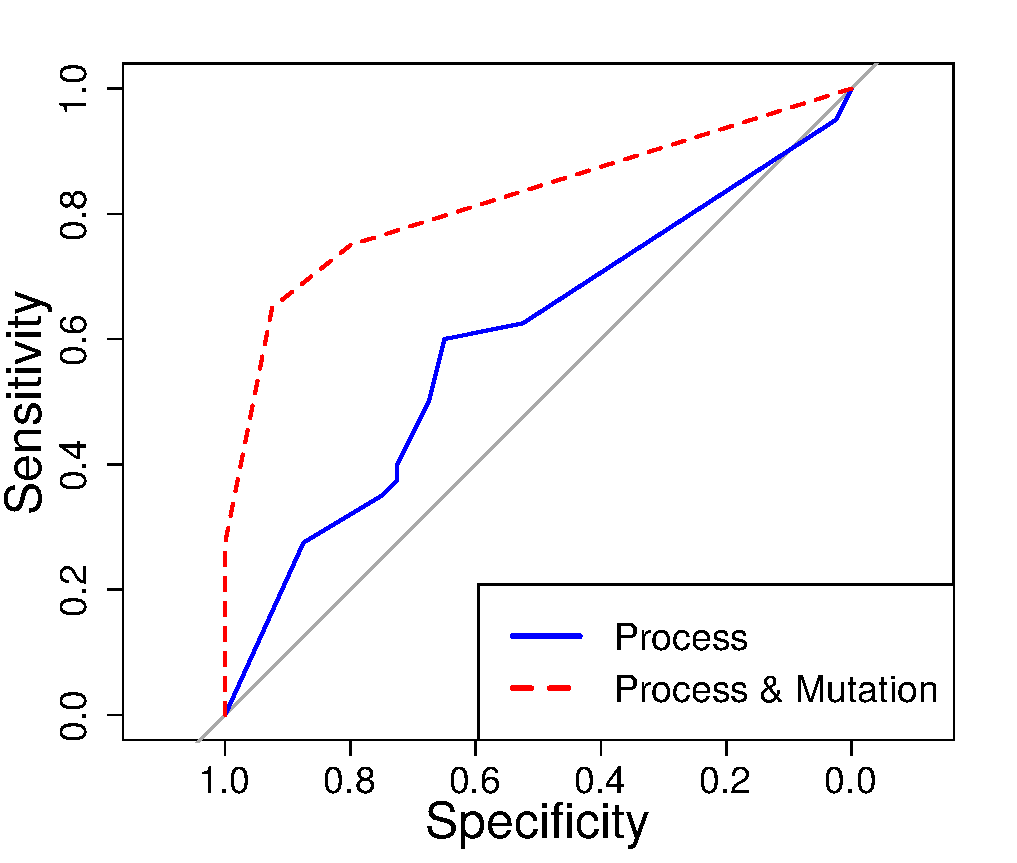
\includegraphics[width=\linewidth]{img/evaluation/phase1-roc-dt.pdf}
		\caption{\lr{Decition Tree}}
	\end{subfigure}
	\begin{subfigure}{.5\textwidth}
	\centering
	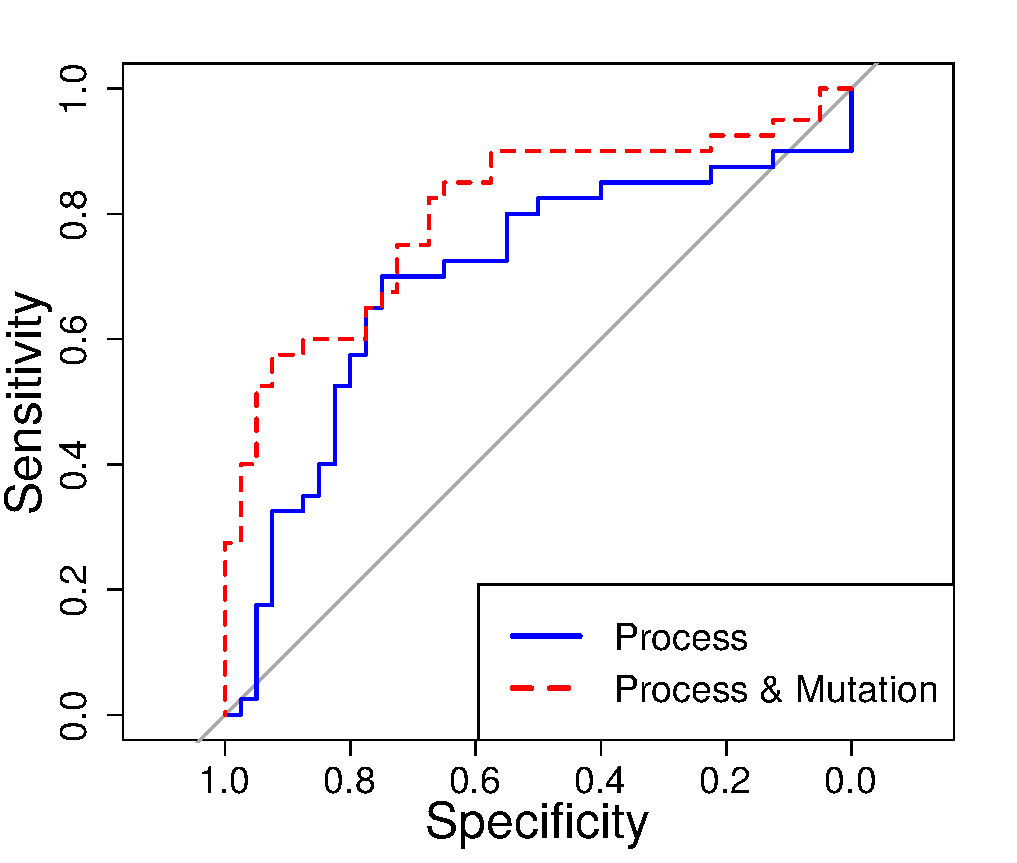
\includegraphics[width=\linewidth]{img/evaluation/phase1-roc-svm.pdf}
	\caption{SVM}
\end{subfigure}
	\begin{subfigure}{.5\textwidth}
	\centering
	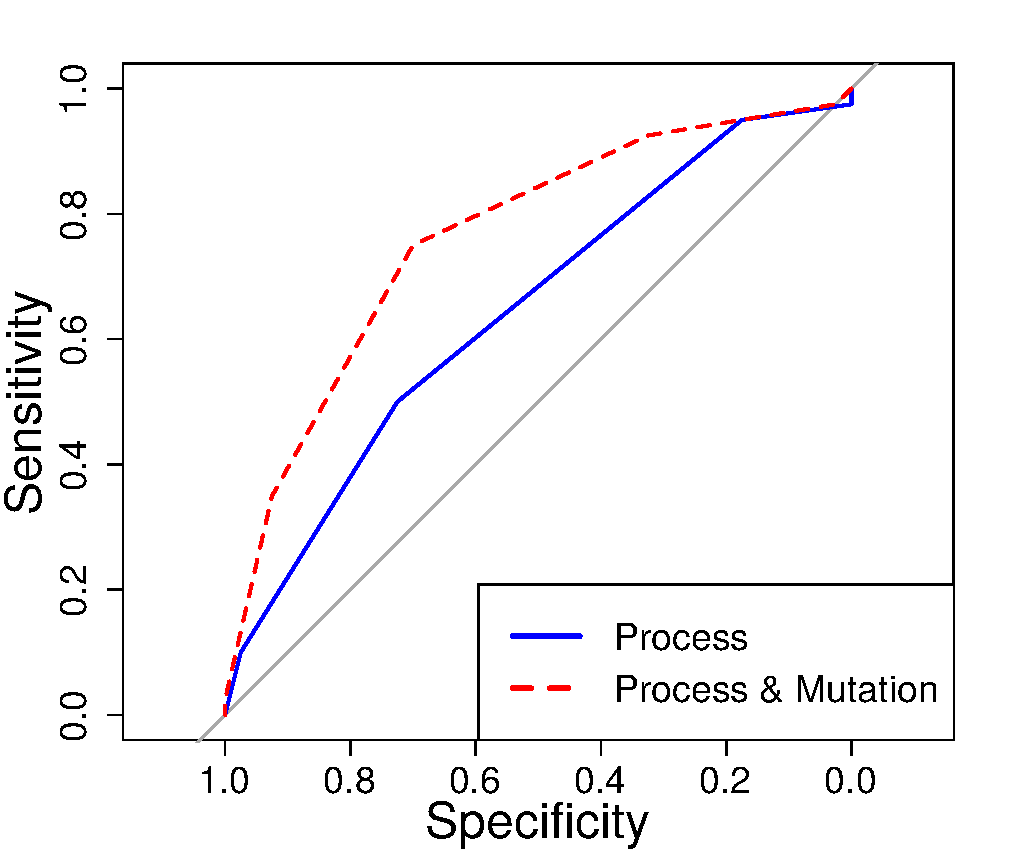
\includegraphics[width= \linewidth]{img/evaluation/phase1-roc-lr.pdf}
	\caption{\lr{Logestic Regression}}
\end{subfigure}
	\begin{subfigure}{.5\textwidth}
	\centering
	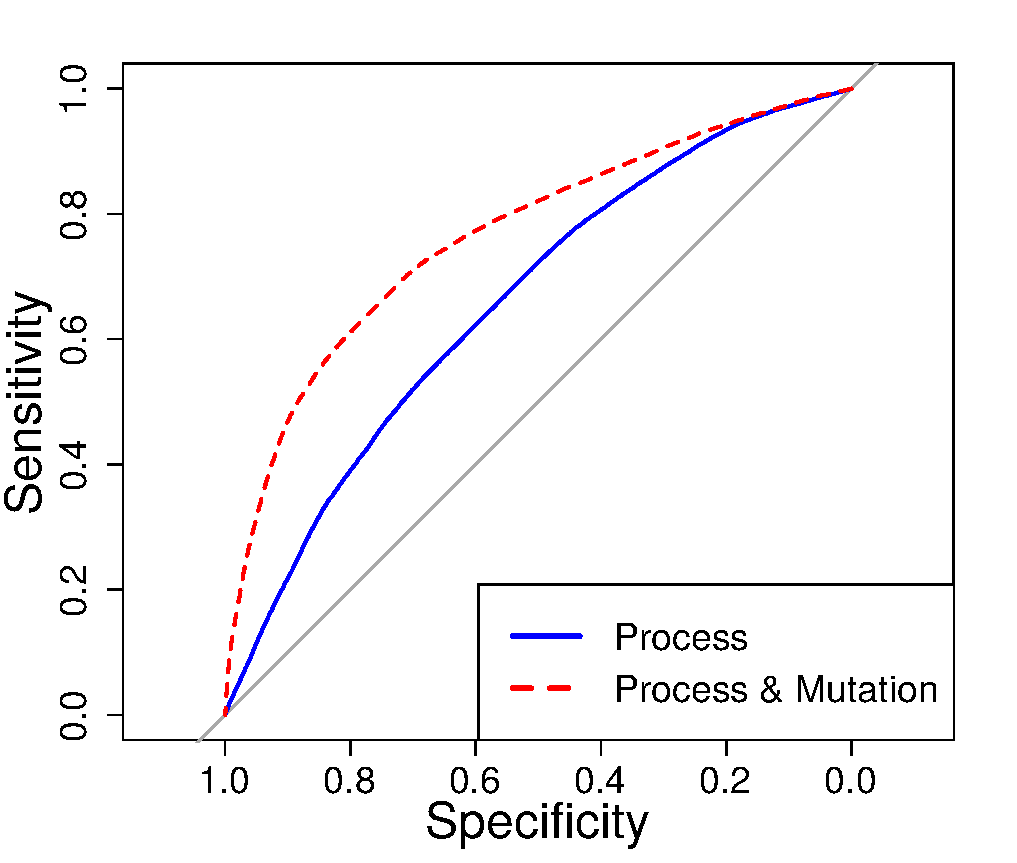
\includegraphics[width= \linewidth]{img/evaluation/phase1-roc-nn.pdf}
	\caption{\lr{Nueral Network}}
\end{subfigure}
\caption{نمودارهای ROC معیارهای فرآیند و به همراه جهش}
\label{fig:ROC-phase1}
\end{figure}

در جدول \ref{tab:auc-phase1} مساحت زیر منحنی ROC در هر یک از روش‌های دسته‌بندی آورده شده است.در میان  روش‌های یادگیری به کار گرفته شده بیشترین افزایش مساحت زیر منحنی را شبکه‌ی عصبی به مقدار $0.226$  واحد داشته است و کمترین  تغییر را نیز  ماشین بردار پشتیبانی با مقدار $0.105$ واحد داشته است.  به طور متوسط  $0.151$ واحد در مدل‌ها بهبود مشاهده می‌شود.  افزایش مساحت زیر منحنی نشانه‌ نزدیکتر شدن به مدل بی‌نقص است و به معنی است که به طور کلی عملکرد بهبود یافته است. این موضوع نشان از تاثیر قابل توجه معیارهای جهش می‌باشد. 

\begin{table}[H] 
	\renewcommand*{\arraystretch}{1.2}	
	\centering \caption{مقادیر زیر نمودار ROC معیارهای فرآیند و به همراه جهش}
	\label{tab:auc-phase1}
	 \rowcolors{2}{blue!15}{white}   
	\begin{tabular}{|c|c|c|c|c|}
		\hline
		\hline
		معیار & 
		 \lr{ Decition Tree} & SVM &\lr{ Logestic Regression} &\lr{ Neural Network} \\
		 \hline
		 \hline
		 فرآیند & 
		 $0.596$ & $0.697$ & $0.643$ & $0.593$
		 \\
		 \hline
		 فرآیند و جهش 
		  & $0.822$ & $0.802$ & $0.761$ & $0.829$
		 \\
		 \hline
		 
	\end{tabular}
\end{table}

\section{ارزیابی معیارهای فرآیند مبتنی بر جهش }
ارزیابی این معیارها در دو مرحله انجام می‌شود. در مرحله‌ی اول  سه  مدل ساخته می‌شود. این مدل‌ها به ترتیب با استفاده از معیارهای فرآیند، فرآیند و جهش و  مدل آخر با استفاده از معیارهای فرآیند و فرآیند مبتنی بر جهش ساخته می‌شود. در مرحله‌ی دوم دو  مدل ساخته می‌شود. در مدل اول معیارهای فرآیند و جهش مدل پیش‌بینی را خواهد ساخت و در مدل دوم معیارهای فرآیند مبتنی بر جهش نیز به مجموعه‌ی معیارها افزوده می‌شود. 

\subsection{مقایسه با معیارهای جهش و فرآیند}
 مقایسه‌ی این مدل‌ها مشخص می‌کند که معیارهای فرآیند مبتنی  بر جهش دارای قابلیت پیش‌بینی هستند یا خیر. همچنین در صورت داشتن این قابلیت مشخص شود که این قابلیت از معیارهای جهش کمتر است یا بیشتر. پارامترهای استفاده شده در مدل سوم در جدول \ref{tab:param2} آمده است. \\
 
  \begin{table}[H] 
 	\renewcommand*{\arraystretch}{1.3}	
 	\centering \caption{پارامترهای مدل ساخته شده}
 	\label{tab:param2}
 	\begin{tabular}{|c|c|}
 		\hline
 		نام روش & پارامتر \\
 		\hline
 		\hline
 		DT & \lr{cp = 0.25}\\
 		\hline
 		SVM & \lr{kernel = polynomial, degree =2, scale=0.1, cost=1}
 		\\
 		\hline
 		LR & - \\
 		\hline
 		NN & \lr{hidden layers = 3, decay=0.1} \\
 		\hline
 		
 	\end{tabular}
 \end{table}
 
مقایسه‌ی نتایج بدست آمده در جدول \ref{tab:eval-phase2-part1}  با جدول \ref{tab:eval-phase1} نشان می‌دهد که در تمامی روش‌های دسته‌بندی  بجز ماشین بردار پشتیبانی معیار صحت در مدل سوم از مدل اول مقدار بیشتری دارد.  در مدل ساخته شده توسط ماشین بردار پشتیبانی نیز اختلاف معیار صحت کم می‌باشد(۳ درصد).  این مدل در مقایسه با مدل دوم عملکرد بهتری از نظر معیار صحت و بازخوانی در هیچکدام از روش‌های دسته‌بندی نداشته است. از نظر معیار دقت  در  تمامی روش‌ها مدل سوم از مدل اول عملکرد بهتری داشته و حتی در روش درخت تصمیم مدل سوم از  مدل دوم نیز بهتر عملکرده است. از نظر معیار بازخوانی مدل سوم نسبت به مدل اول تنها در روش شبکه‌ی عصبی عملکرد بهتری داشته، در درخت تصمیم بدون تغییر مانده و در دو روش دیگر کاهش یافته است. \\
می‌توان این نتیجه را برداشت کرد که معیارهای ارائه شده دارای توانایی پیش‌بینی بیشتری نسبت به معیارهای فرآیند به تنهایی هستند.
 \\
 
 
 \begin{table}[H] 
 	\renewcommand*{\arraystretch}{1.3}	
 	\centering \caption{نتایج پیش‌بینی‌خطای معیارهای فرآیند مبتنی بر جهش - مرحله‌ی اول} 
 	\label{tab:eval-phase2-part1}

 	\begin{tabular}{|c|c|c|c|}
 		
 		\hline
 		\hline
 		 نام روش  & صحت & دقت & بازخوانی	
 		\\
 		\hline
 		\hline
 		 
 		\lr{Decition Tree} & $0.725 $&$0.750$&$0.675$
 		\\
 		\hline
 	
 		\lr{SVM} & $0.637$&$0.689$&$0.500$
 		
 		\\
 		\hline
 	 
 		\lr{Logestic Regression} & $0.662$&$0.685$&$0.600$
 		\\
 		\hline
 	 
 		\lr{Neural Network} & $0.762$&$0.756$&$0.775$
 		\\
 		\hline
	\end{tabular}
 \end{table}


در شکل \ref{fig:ROC-phase2-part1} نمودارهای ROC سه مدل ساخته شده نشان داده شده است. در زیرشکل‌های (آ)(ج)(د) به وضوح عملکرد بهتر مدل سوم از مدل اول قابل مشاهده است. در زیرشکل (ب)نیز که متعلق به ماشین بردار پشتیبانی است با رجوع به جدول \ref{tab:auc-phase2-part1} مشخص می‌شود که در این شکل نیز مساحت زیر منحنی ROC در مدل سوم بیشتر از اول است. همچنین مساحت زیر منحنی در مدل سوم در زیرشکل (ج) به مقدار $0.015$ واحد از مدل دوم نیز بیشتر است. 

این نتایج در راستای نتایج بدست آمده از جدول \ref{tab:eval-phase2-part1} می‌باشد. در نهایت می‌توان این نتیجه را گرفت که معیارهای فرآیند مبتنی بر جهش معرفی شده پیش‌بینی خطا را بهبود می‌بخشند  اما عملکرد بهتری نسبت به معیارهای جهش ندارند. همچنین از آنجا که هزینه‌ی محاسباتی بیشتری نسبت به معیارهای جهش دارند جایگزینی آنها به جای یکدیگر مزیتی ندارد. 

\begin{figure}[H]
	\begin{subfigure}{.5\textwidth}
		\centering
		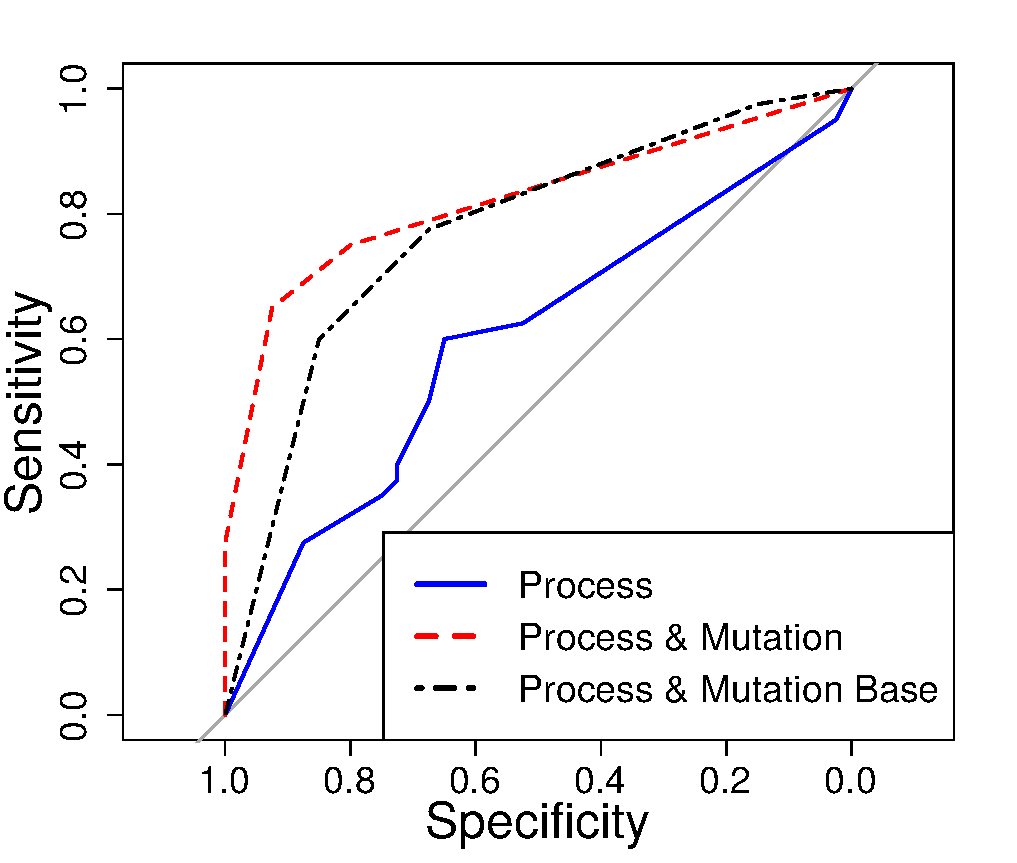
\includegraphics[width=\linewidth]{img/evaluation/phase2-part1-roc-dt.pdf}
		\caption{\lr{Decition Tree}}
	\end{subfigure}
	\begin{subfigure}{.5\textwidth}
		\centering
		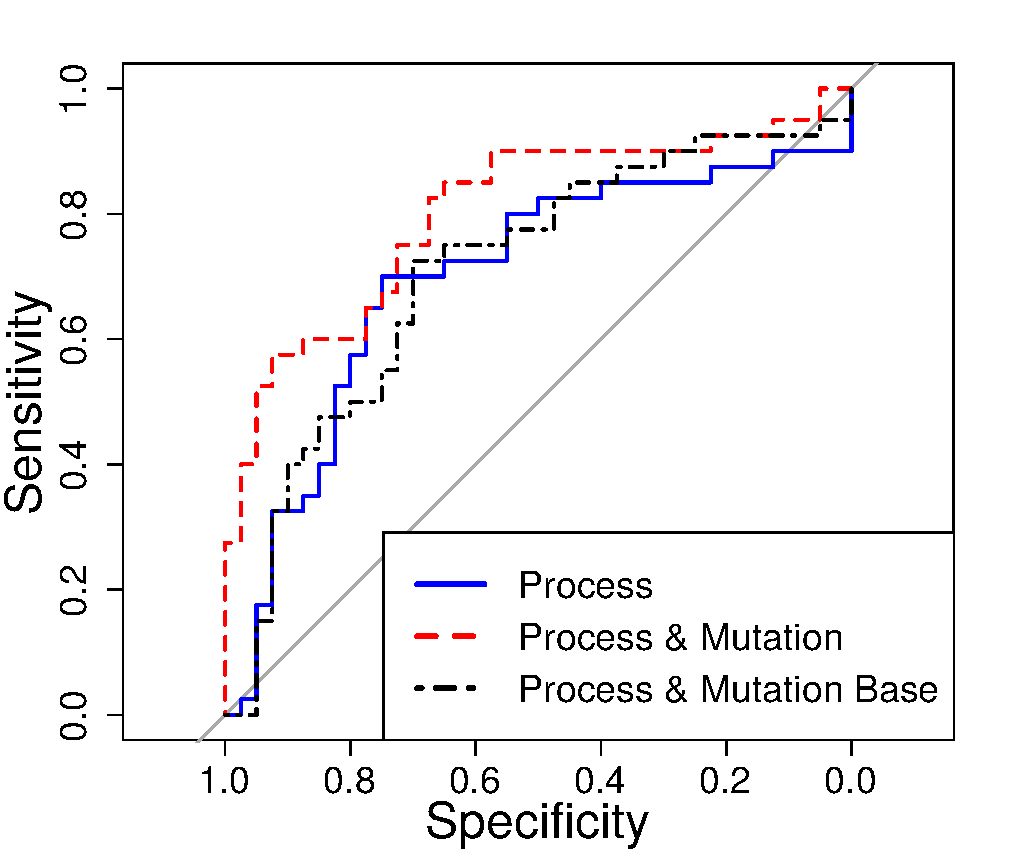
\includegraphics[width=\linewidth]{img/evaluation/phase2-part1-roc-svm.pdf}
		\caption{SVM}
	\end{subfigure}
	\begin{subfigure}{.5\textwidth}
		\centering
		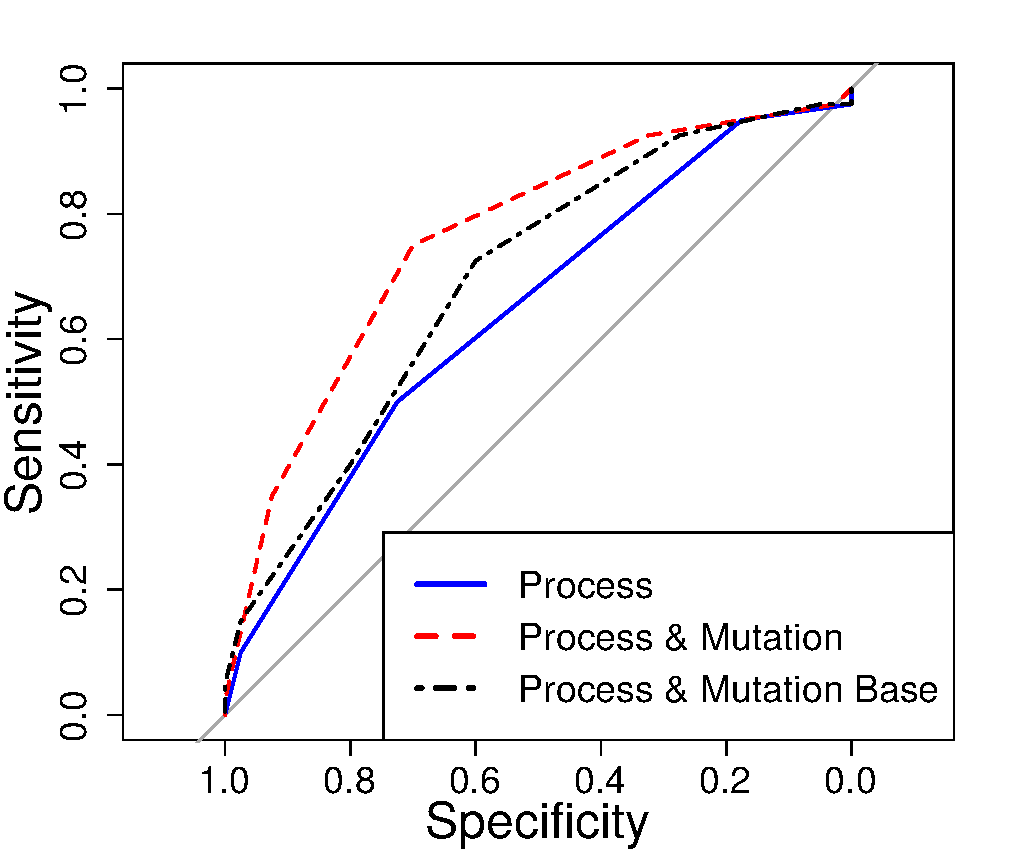
\includegraphics[width= \linewidth]{img/evaluation/phase2-part1-roc-lr.pdf}
		\caption{\lr{Logestic Regression}}
	\end{subfigure}
	\begin{subfigure}{.5\textwidth}
		\centering
		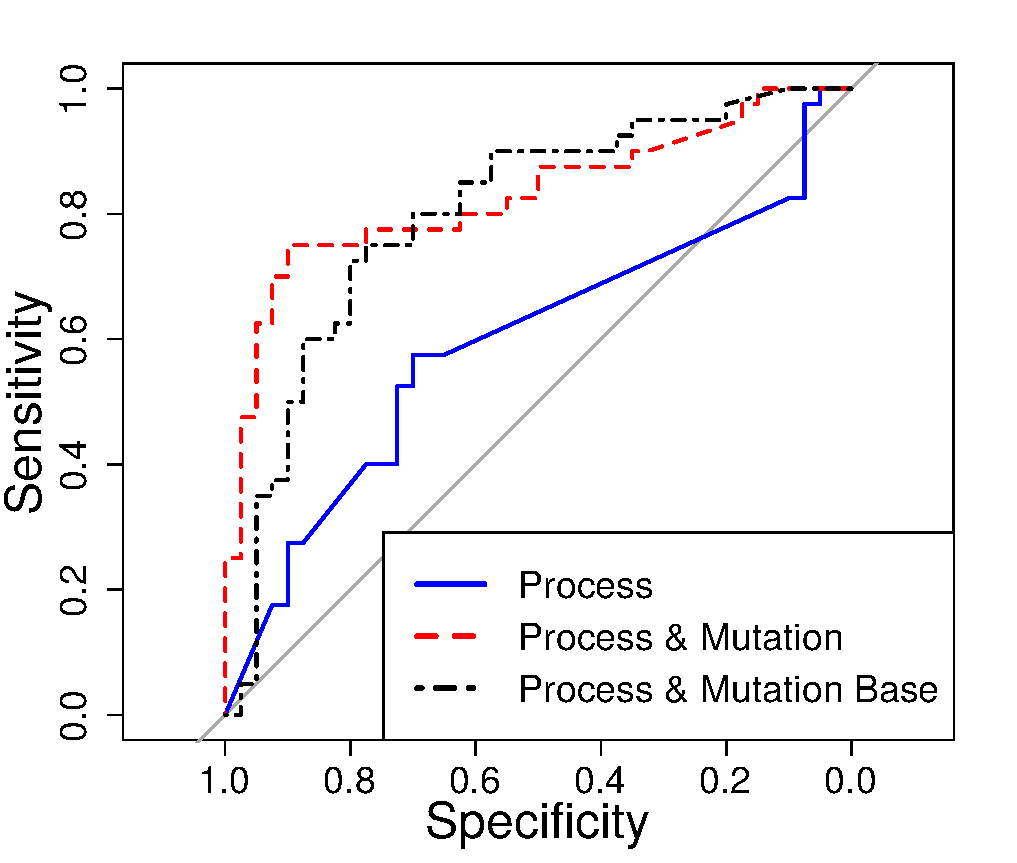
\includegraphics[width= \linewidth]{img/evaluation/phase2-part1-roc-nn.pdf}
		\caption{\lr{Nueral Network}}
	\end{subfigure}
	\caption{نمودارهای ROC معیارهای فرآیند ، فرآیند و جهش ، فرآیند مبتنی بر جهش}
	\label{fig:ROC-phase2-part1}
\end{figure}

\begin{table}[H] 
	\renewcommand*{\arraystretch}{1.2}	
	\centering \caption{مقادیر زیر نمودار ROC معیارهای فرآیند مبتنی جهش}
	\label{tab:auc-phase2-part1}
	\begin{tabular}{|c|c|c|c|}
		\hline
		\hline
		 
		\lr{ Decition Tree} & SVM &\lr{ Logestic Regression} &\lr{ Neural Network} \\
		\hline
		\hline
		 $0.772$ & $0.707$ & $0.693$ & $0.798$
		\\
		\hline
	
		
	\end{tabular}
\end{table}

\subsection{قرارگیری همگی معیارها در کنار هم}
همانطور که اشاره شد دو مدل ساخته می‌شود که مدل اول از معیارهای فرآیند و جهش استفاده می‌کند و در مدل دوم  از همگی معیارها (با افزودن معیارهای فرآیند مبتنی بر جهش) استفاده می‌شود. هدف از این آزمایش این است که مشخص شود در صورتی که معیارهای ارائه شده‌ی جدید در کنار معیارهای قبلی قرار گیرد، در پیش‌بینی بهبودی حاصل می‌گردد یا خیر. پارامترهای استفاده شده در مدل دوم در جدول \ref{tab:param3} آمده است. 

 \begin{table}[H] 
	\renewcommand*{\arraystretch}{1.3}	
	\centering \caption{پارامترهای مدل ساخته شده}
	\label{tab:param3}
	\begin{tabular}{|c|c|}
		\hline
		نام روش & پارامتر \\
		\hline
		\hline
		DT & \lr{cp = 0.156}\\
		\hline
		SVM & \lr{kernel = polynomial, degree =3, scale=0.1, cost=0.5}
		\\
		\hline
		LR & - \\
		\hline
		NN & \lr{hidden layers = 3, decay=0.1} \\
		\hline
		
	\end{tabular}
\end{table}

نتایج بدست آمد در جدول \ref{tab:eval-phase2-part2} نشان می‌دهد که مدل دوم  در هیچ یک از روش‌ها بجز رگرسیون منطقی از نظر معیارهای صحت، دقت و بازخوانی نسبت به مدل اول بهبودی پیدا نکرده است. همچنین در روش درخت تصمیم نتایج دو مدل یکسان است.  در روش رگرسیون منطقی مدل دوم در معیار صحت $1.2$ درصد افزایش، در معیار دقت $5$ درصد کاهش و $17.5$ درصد در بازخوانی افزایش داشته است. 

 \begin{table}[H] 
	\renewcommand*{\arraystretch}{1.3}	
	\centering \caption{نتایج پیش‌بینی خطای مدل حاصل از بکارگیری تمامی معیارها}
	\label{tab:eval-phase2-part2}
	
	\begin{tabular}{|c|c|c|c|}
		
		\hline
		\hline
		نام روش  & صحت & دقت & بازخوانی	
		\\
		\hline
		\hline
		
		\lr{Decition Tree} & $0.787$&$0.725$&$0.925$
		\\
		\hline
		
		\lr{SVM} & $0.712$&$0.774$&$0.600$
		\\
		\hline
		
		\lr{Logestic Regression} & $0.737 $&$0.686$&$0.875$
		\\
		\hline
		
		\lr{Nueral Network} & $0.750$&$0.717$&$0.825$
		\\
		\hline
	\end{tabular}
\end{table}
 
 نمودارهای ROC هر یک از این دو مدل در روش‌های دسته‌بندی مختلف در شکل \ref{fig:ROC-phase2-part2} آمده است. در روش‌های مختلف مدل اول با دوم تفاوت چندانی ندارند و طبق جدول \ref{tab:auc-phase2-part2} تنها در مدل‌های حاصل از روش رگرسیون منطقی به مقدار $0.009$ واحد مساحت زیر منحنی افزایش پیدا  کرده است. بنابرین افزودن  معیارهای فرآیند مبتنی بر جهش به سایر معیارهای مورد بررسی نمی‌تواند به بهبود پیش‌بینی بیانجامد.
\begin{figure}[H]
	\begin{subfigure}{.5\textwidth}
		\centering
		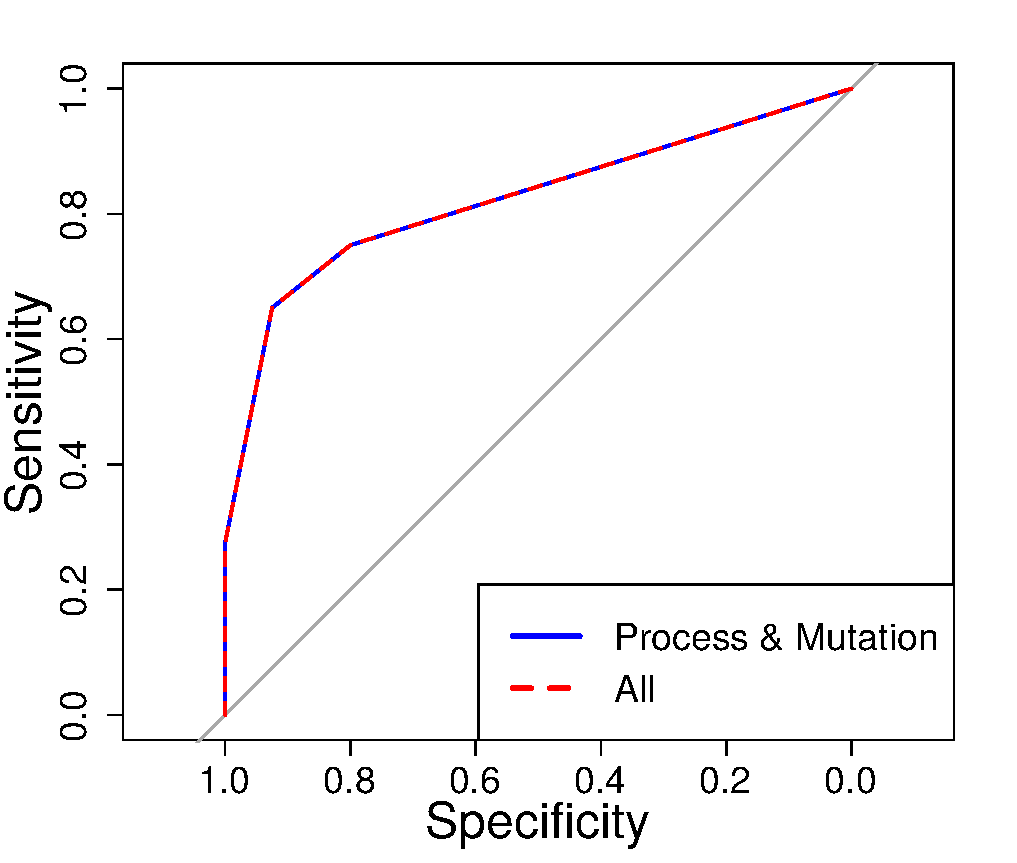
\includegraphics[width=\linewidth]{img/evaluation/phase2-part2-roc-dt.pdf}
		\caption{\lr{Decition Tree}}
	\end{subfigure}
	\begin{subfigure}{.5\textwidth}
		\centering
		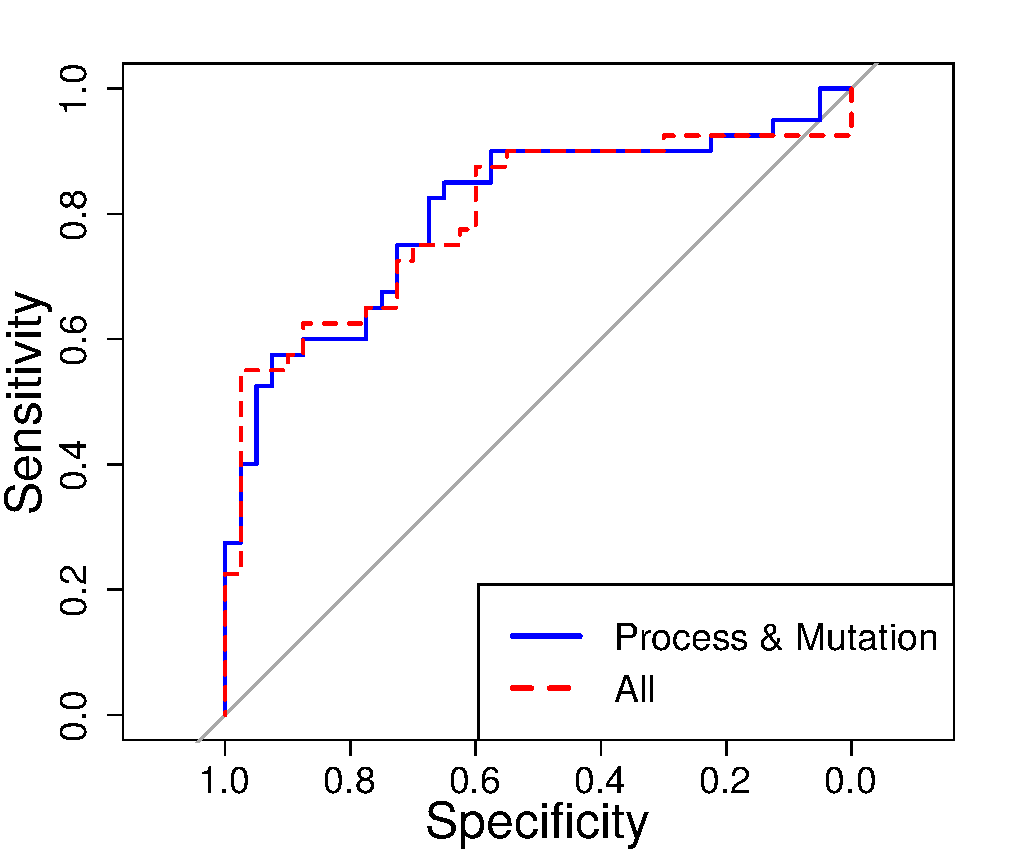
\includegraphics[width=\linewidth]{img/evaluation/phase2-part2-roc-svm.pdf}
		\caption{SVM}
	\end{subfigure}
	\begin{subfigure}{.5\textwidth}
		\centering
		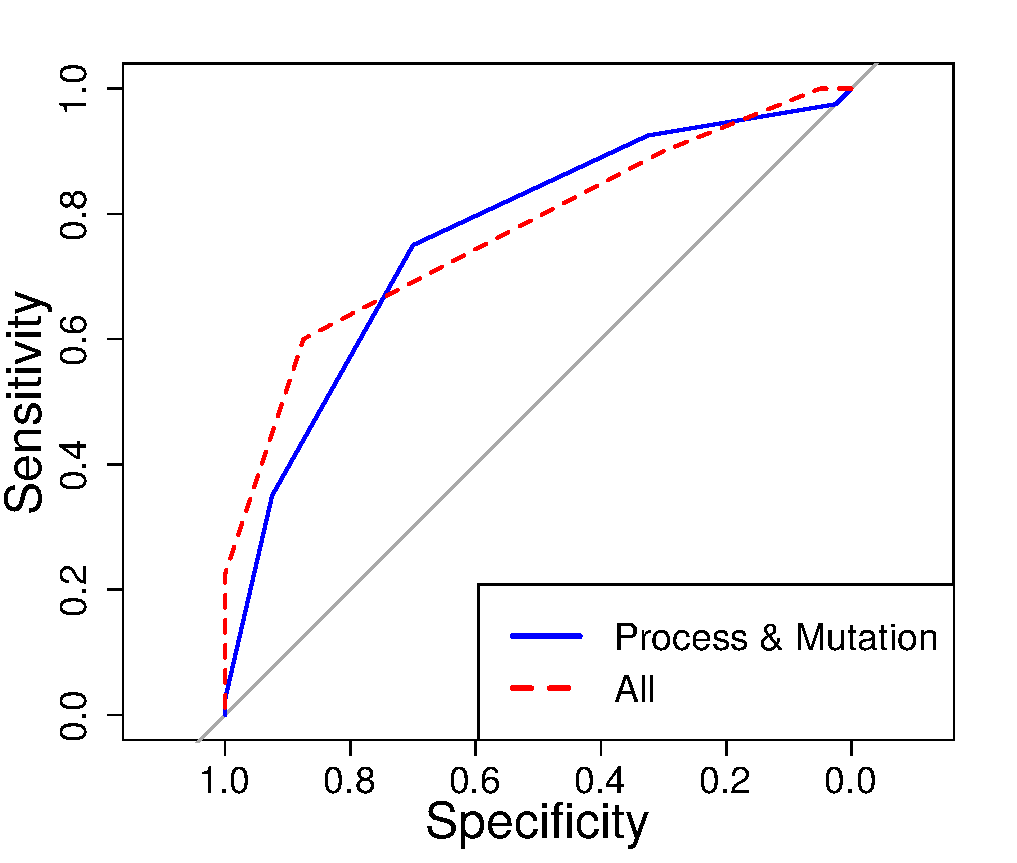
\includegraphics[width= \linewidth]{img/evaluation/phase2-part2-roc-lr.pdf}
		\caption{\lr{Logestic Regression}}
	\end{subfigure}
	\begin{subfigure}{.5\textwidth}
		\centering
		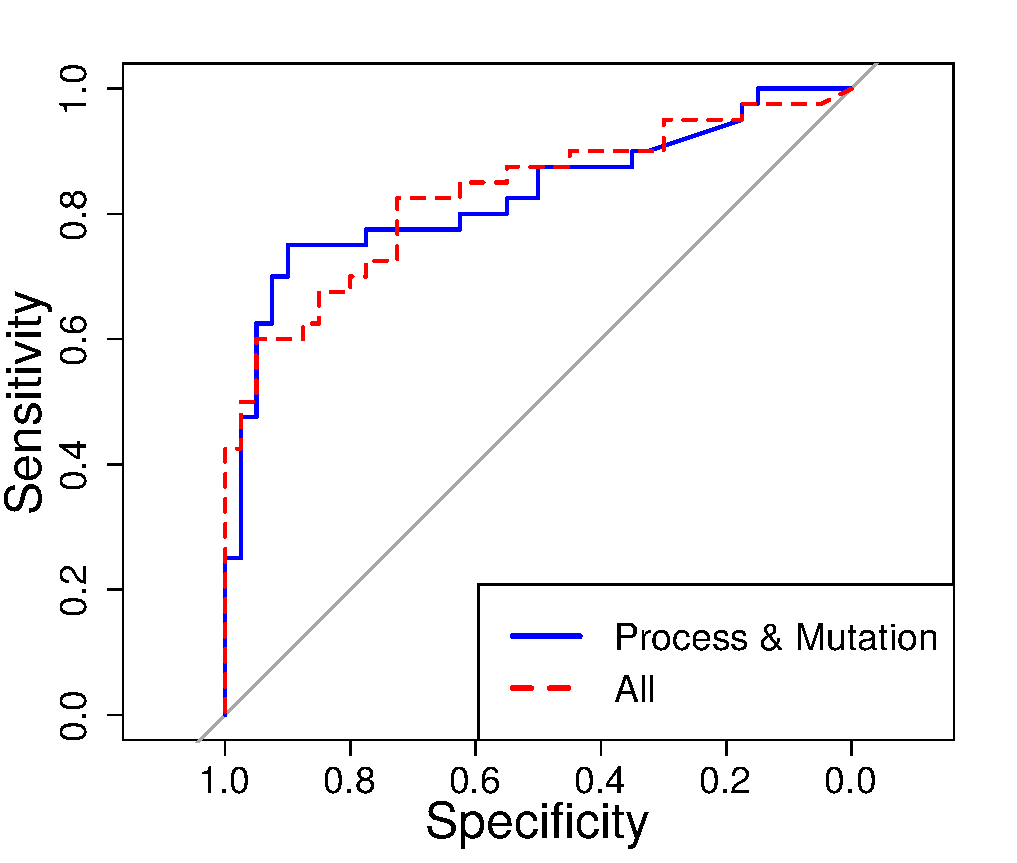
\includegraphics[width= \linewidth]{img/evaluation/phase2-part2-roc-nn.pdf}
		\caption{\lr{Nueral Network}}
	\end{subfigure}
	\caption{نمودارهای ROC معیارهای جهش و فرآیند و تمامی معیارها }
	\label{fig:ROC-phase2-part2}
\end{figure}

\begin{table}[H] 
	\renewcommand*{\arraystretch}{1.2}	
	\centering \caption{مقادیر زیر نمودار ROC تمامی معیارها}
	\label{tab:auc-phase2-part2}
	\begin{tabular}{|c|c|c|c|}
		\hline
		\hline
		
		\lr{ Decition Tree} & SVM &\lr{ Logestic Regression} &\lr{ Neural Network} \\
		\hline
		\hline
		$0.822$ & $0.786$ & $0.770$ & $0.830$
		\\
		\hline
		
		
	\end{tabular}
\end{table}

\section{ارزیابی معیارهای ترکیبی فرآیند-جهش}
 در این قسمت به ارزیابی دو معیار مطرح شده پرداخته می‌شود. به منظور ارزیابی آنها دو مدل با استفاده از هر یک از روش‌های دسته‌بندی ساخته می‌شود. در مدل اول معیارهای فرآیند استفاده می‌شود و در مدل دوم معیار \موکد{مقدار نرمال شده‌ی خطوط اضافه شده} \ref{eq:added_line} با معیار \موکد{تعداد خطوط اضافی وزن‌دهی شده} \ref{eq:n_add_line} جایگزین می‌شود و معیار \موکد{مقدار نرمال شده‌ی خطوط حذف شده}  \ref{eq:deleted_line} نیز به طور مشابه   با \ref{eq:n_delete_line} جایگزین می‌شود. سایر معیارهای مدل دوم با مدل اول یکسان خواهد بود. پارامترهای استفاده شده در  مدل دوم در جدول \ref{tab:param4} آمده است. 
 
 \begin{table}[H] 
 	\renewcommand*{\arraystretch}{1.3}	
 	\centering \caption{پارامترهای مدل ساخته شده}
  \label{tab:param4}
	 \begin{tabular}{|c|c|}
 		\hline
 		نام روش & پارامتر \\
 		\hline
 		\hline
 		DT & \lr{cp = 0.170}\\
 		\hline
 		SVM & \lr{kernel = polynomial, degree =2, scale=0.1, cost=0.25}
 		\\
 		\hline
 		LR & - \\
 		\hline
 		NN & \lr{hidden layers = 3, decay=0.1} \\
 		\hline
 		
 	\end{tabular}
\end{table}
 

 نتایج به دست آمده در جدول \ref{tab:eval-phase3} نشان می‌دهد که معیارهای صحت، دقت و بازخوانی برای تمامی مدل‌ها بجز مدل ساخته شده توسط روش ماشین بردار پشتیبانی افزایش قابل ملاحظه‌ای داشته است. بیشترین افزایش صحت در روش شبکه‌ی عصبی به میزان $13.8$ درصد روی داده است. از نظر افزایش دقت بیشترین تغییر مثبت در روش درخت تصمیم بوده است که $13.1$ درصد رشد داشته است. معیار بازخوانی در دو  روش رگرسیون منطقی و شبکه‌ی عصبی به ترتیب $8.4$ و $2.5$ رشد داشته و در دو روش دیگر کاهش داشته است. \\
 به طور میانگین معیار صحت $6.6$ درصد افزایش، معیار دقت $6$ درصد افزایش  و معیار بازخوانی $0.4$ درصد کاهش داشته است. در نهایت می‌توان این نتیجه را گرفت که معیارهای ترکیبی جهش-فرآیند موجب بهبود در صحت و دقت پیش‌بینی می‌شوند و تاثیر چندانی در بازخوانی ندارند. لازم به ذکر است که تنها دو معیار از ۱۲ معیار مورد استفاده در دو مدل ساخته شده با هم متفاوت هستند که این دو معیار توانسته‌اند حدود $6$ درصد صحت و دقت را بهبود بخشند. این امر نشان از تاثیر قابل ملاحظه‌ی این معیارها می‌باشد. \\
 \begin{table}[H] 
 	\renewcommand*{\arraystretch}{1.3}	
 	\centering \caption{مقایسه‌ی معیارهای فرآیند و معیارهای 
 		ترکیبی جهش-فرآیند}
  	\rowcolors{4}{blue!15}{white}  
 	\label{tab:eval-phase3}

 	\begin{tabular}{|c|C{1cm}|C{1cm}|C{1.2cm}|C{1cm}|C{1cm}|C{1.2cm}|C{1cm}|C{1cm}|C{1.2cm}|}
 		
 		\hline
 		\hline
 		\multirow{2}{*}{نام روش} &
 		\multicolumn{3}{c|}{صحت} &
 		\multicolumn{3}{c|}{دقت} &
 		\multicolumn{3}{c|}{بازخوانی} \\
 		\cline{2-10}
 	&	P & \lr{MPH} & Diff & P & \lr{MPH} & Diff & P & \lr{MPH} & Diff\\
 		\hline
 		\hline
 		 
 DT &$0.587$ &	$0.675$ &	$+0.088$
 &$0.574$&	$0.705$&$+0.131$
 &$0.675$	&$0.600$	&$-0.075$ 
 \\
\hline
SVM &$0.662$ &	$0.637$&	$-0.02$
&$0.685$&	$0.666$&$-0.019$ &
$0.600	$&$0.550$&	$-0.025$
 \\
\hline
LR &$0.612$&$0.675$&$+0.063$
&$0.591$&$0.652$&$+0.061$
&$0.725$&$0.750$&$+0.025$
\\
\hline
NN‌&$0.612$&$0.750$&	$+0.138$
&$0.725$	&$0.794$&$	+0.069$
&$0.591$	&$0.675$&$	+0.084$
\\
\hline

 	\end{tabular}
 \end{table}
 

\begin{comment}

\begin{table}[H] 
	\renewcommand*{\arraystretch}{1.3}	
	\centering \caption{مقایسه‌ی معیارهای فرآیند و معیارهای ترکیبی جهش-فرآیند}
	\label{tab:eval-phase3-old}
	\rowcolors{2}{blue!15}{white}   
	\begin{tabular}{|c|c|c|c|c|}
		
		\hline
		\hline
		معیار & نام روش  & صحت & دقت & بازخوانی	
		\\
		\hline
		\hline
		فرآیند & 
		\lr{Decition Tree} & $0.587$&$0.574$&$0.675$
		\\
		\hline
		ترکیبی جهش-فرآیند& 
		\lr{Decition Tree} & $0.675$&$0.705$&$0.600$
		\\
		\hline
		فرآیند & 
		\lr{SVM} & $0.662$&$0.685$&$0.600$
		\\
		\hline
		ترکیبی جهش-فرآیند & 
		\lr{SVM} & $0.637$&$0.666$&$0.550$
		\\
		
		\hline
		فرآیند &
		\lr{Logestic Regression} & $0.612$&$0.591$&$0.725$
		\\
		\hline
		ترکیبی جهش-فرآیند & 
		\lr{Logestic Regression} & $0.675 $&$0.652$&$0.750$
		\\
		\hline
		فرآیند &
		\lr{Nueral Network} & $0.612$&$0.725$&$0.591$
		\\
		\hline
		ترکیبی جهش-فرآیند & 
		\lr{Nueral Network} & $0.750$&$0.794$&$0.675$
		\\
		\hline		
	\end{tabular}
\end{table}
\end{comment}
در شکل \ref{fig:ROC-phase3} نمودارهای ROC به تفکیک روش دسته‌بندی آمده است. در هر یک از زیر شکل‌ها منحنی ROC مربوط به  دو مدل با هم مقایسه شده است. درمدل اول که در ساخت آن از معیارهای فرآیند استفاده شده  با خط ممتد نمایش داده شده است و مدل دوم  از جایگزینی دو معیار فرآیند با معیارهای ترکیبی جهش-فرآیند ساخته شده و با خط چین نمایش داده شده‌. همانطور که قابل مشاهده است در تمامی روش‌ها بجز  ماشین بردار پشتیبانی مدل‌ دوم مساحت زیر منحنی بیشتری نسبت به مدل اول داشته است.
\begin{figure}[H]
	\begin{subfigure}{.5\textwidth}
		\centering
		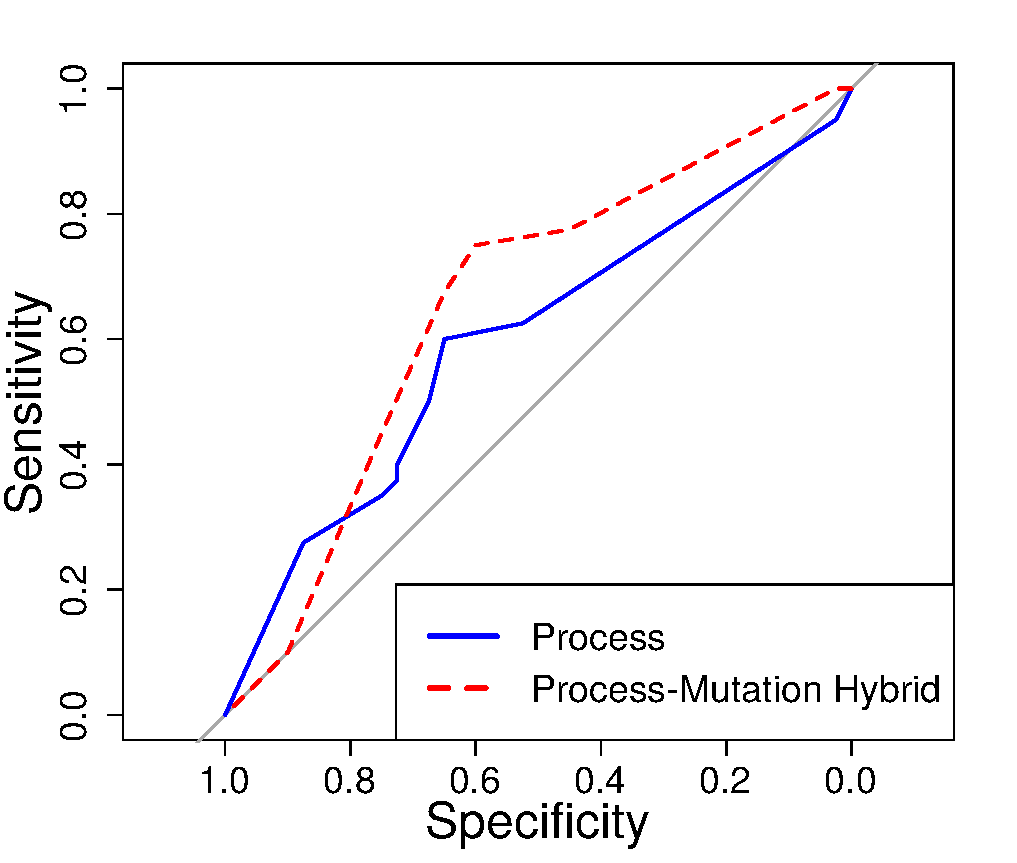
\includegraphics[width=\linewidth]{img/evaluation/phase3-roc-dt.pdf}
		\caption{\lr{Decition Tree}}
	\end{subfigure}
	\begin{subfigure}{.5\textwidth}
		\centering
		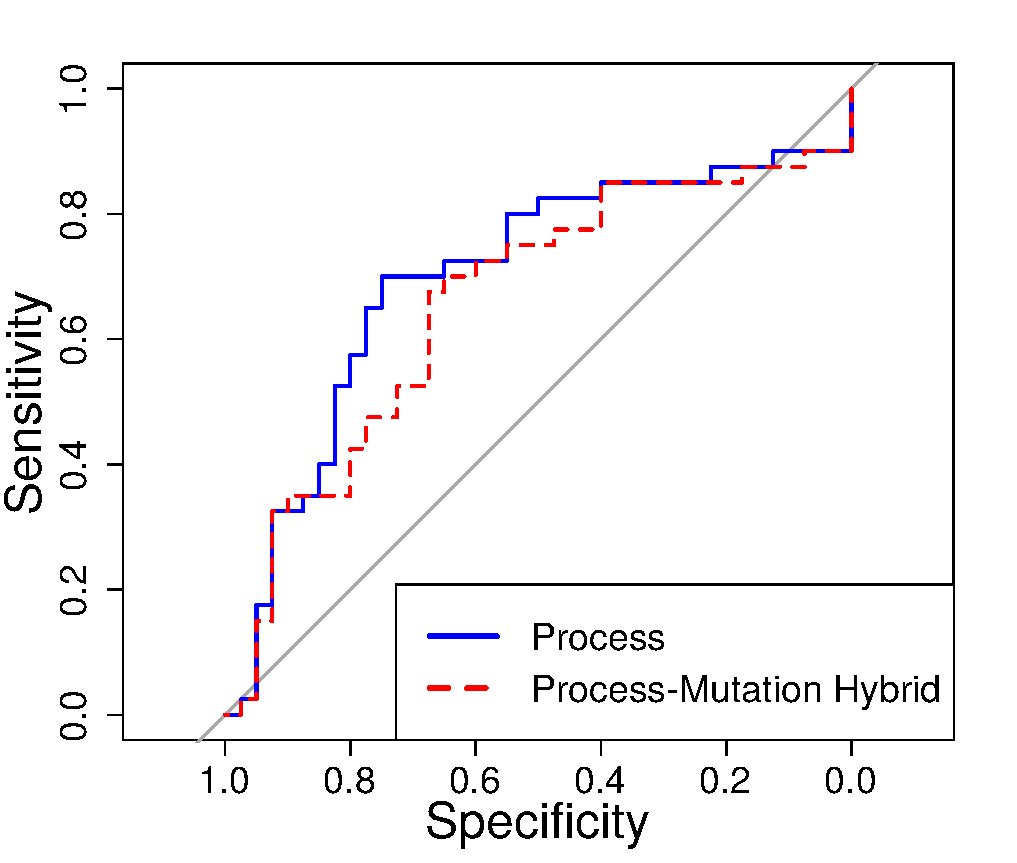
\includegraphics[width=\linewidth]{img/evaluation/phase3-roc-svm.pdf}
		\caption{SVM}
	\end{subfigure}
	\begin{subfigure}{.5\textwidth}
		\centering
		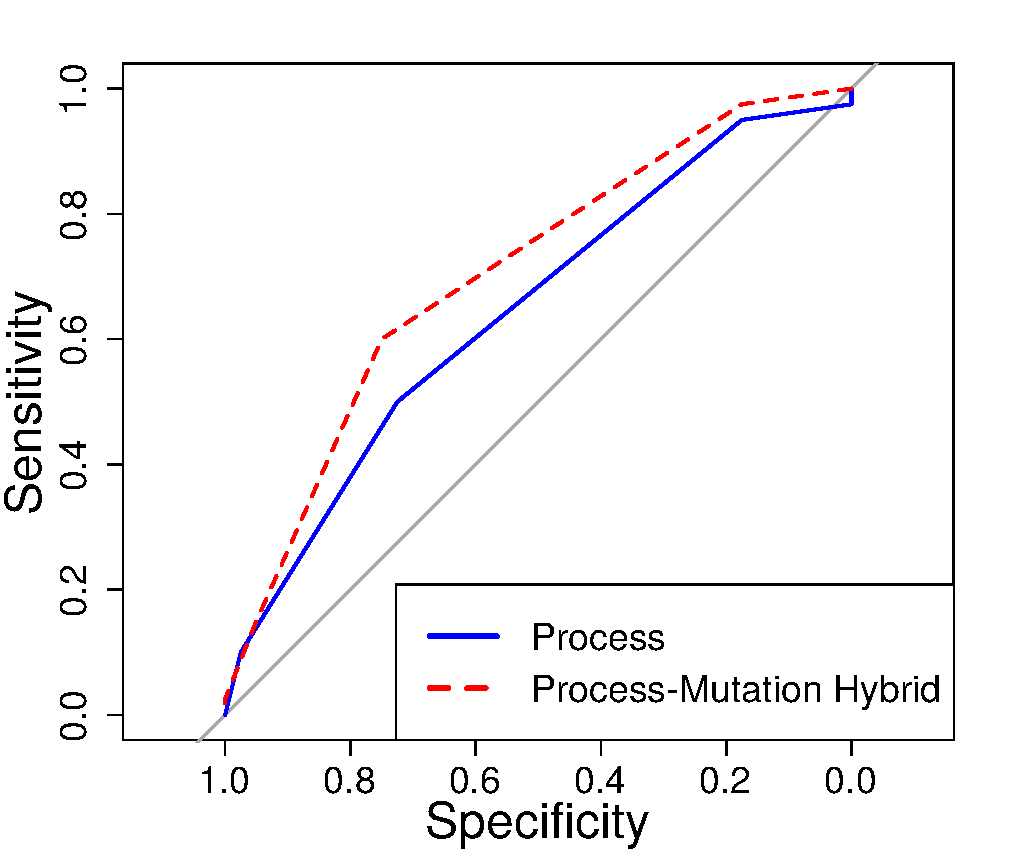
\includegraphics[width= \linewidth]{img/evaluation/phase3-roc-lr.pdf}
		\caption{\lr{Logestic Regression}}
	\end{subfigure}
	\begin{subfigure}{.5\textwidth}
		\centering
		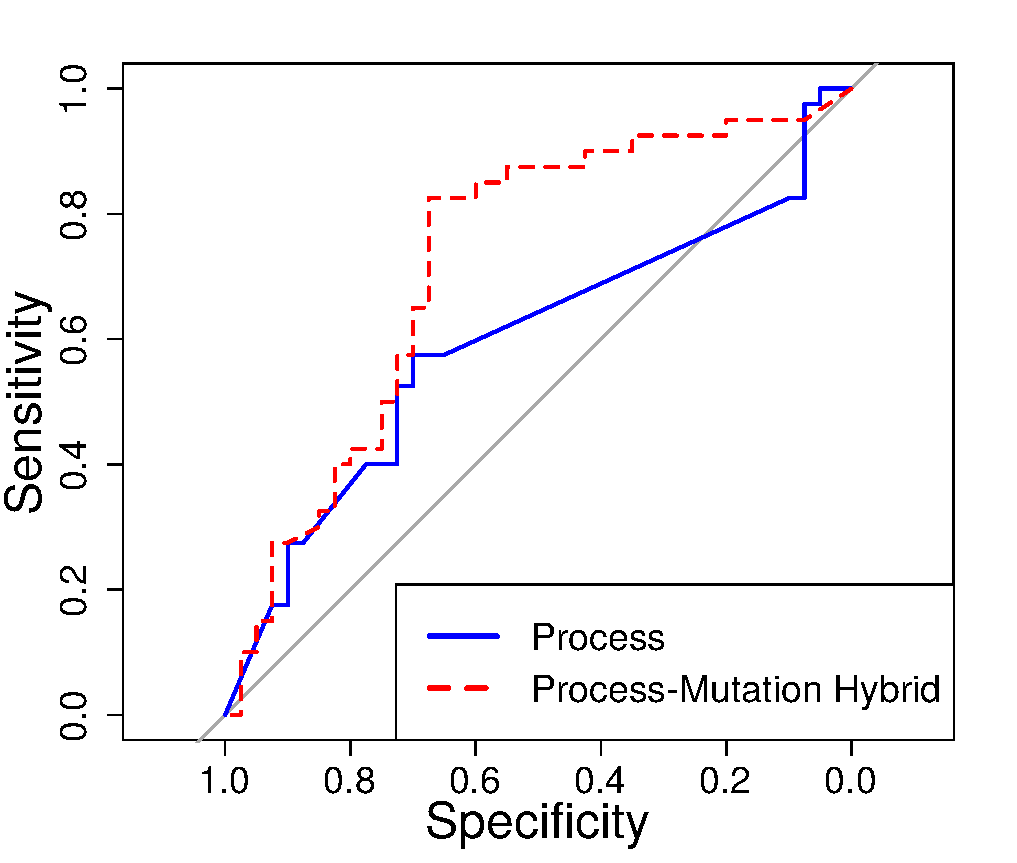
\includegraphics[width= \linewidth]{img/evaluation/phase3-roc-nn.pdf}
		\caption{\lr{Nueral Network}}
	\end{subfigure}
	\caption{نمودارهای ROC معیارهای فرآیند و به همراه جهش}
	\label{fig:ROC-phase3}
\end{figure}

در جدول \ref{tab:auc-phase3} مساحت زیر منحنی ROC  دو مدل به تفکیک روش دسته‌بندی آورده شده است. در میان  روش‌های یادگیری به کار گرفته شده بیشترین افزایش مساحت زیر منحنی را روش  شبکه‌ی عصبی به مقدار $0.128$  واحد داشته است. به طور متوسط  $0.051$ واحد در مدل‌ها بهبود مشاهده می‌شود. این موضوع نشان می‌دهد که معیارهای ترکیبی جهش-فرآیند از نظر مساحت زیر منحنی ROC نیز موجب تغییر مثبت ایجاد می‌شوند. \\

با توجه به اینکه تنها روش ماشین بردار پشتیبانی  نتایج ضعیفی نسبت به سایرین داشته است این موضوع را می‌توان با توجه نحوه‌ی عملکرد این روش توجیه کرد. به طور خلاصه این روش سعی می‌کند که  \واژه{فضای ویژگی}  را با ایجاد یک \واژه{ابرصفحه} به دسته‌های مختلف تقسیم کند اما توزیع نقاط داده در فضای ویژگی به نحوی نیست که این روش بتواند به خوبی عمل کند. 

\begin{table}[H] 
	\renewcommand*{\arraystretch}{1.2}	
	\centering \caption{مقادیر زیر نمودار ROC معیارهای فرآیند و معیارهای ترکیبی جهش-فرآیند}
	\label{tab:auc-phase3}
	\rowcolors{2}{blue!15}{white}   
	\begin{tabular}{|c|c|c|c|c|}
		\hline
		\hline
		معیار & 
		\lr{ Decition Tree} & SVM &\lr{ Logestic Regression} &\lr{ Neural Network} \\
		\hline
		\hline
		فرآیند
		 & $0.596$ & $0.697$ & $0.643$ & $0.593$
		\\
		\hline
		جهش-فرآیند  
		& $0.654$ & $0.656$ & $0.705$ & $0.721$
		\\
		\hline
		
	\end{tabular}
\end{table}
\فصل{نتیجه‌گیری و کارهای آتی}
\برچسب{chap:future}
در این پژوهش سعی شد که تاثیر معیار‌های جهش پیش‌بینی خطا بر پیش‌خطا در هنگام قرار گیری در کنار معیار‌های فرآیند ارزیابی  شود و معیارهای جدیدی با استفاده از مفاهیم تحلیل جهش و تاریخچه‌ی توسعه‌ی نرم‌افزار ارائه گردد. در فصل \ref{chap:intro} به بیان مسئله و مفاهیم مقدماتی پرداخته شد. در فصل \ref{chap:survey}  پژوهش‌های پیشین در حوزه‌ی پیش‌بینی خطا مورد بررسی قرار گرفت. پژوهشگران به طرق مختلف سعی در دستیابی به نتایج بهتری در پیش‌بینی خطا هستند. در این بررسی مشخص شد که در پژوهش‌های پیشین دو دسته‌ی کلی از معیارها مورد استفاده قرار گرفته است. این دسته‌ها عبارتند از معیارهای کد و معیارهای فرآیند. معیارهای فرآیند دارای مزیت‌ها بیشتری نسبت به معیارهای کد هستند و پژوهش‌های کمتری نیز به بررسی آنها پرداخته است. در یکی از پژوهش‌های اخیر از معیارهای جهش  در کنار معیارهای کد به منظور پیش‌بینی‌خطا استفاده گردیده و موجب بهبود پیس‌بینی شده است. \\

پس از مشخص شدن بخش‌هایی از این حوزه که نیازمند تحقیق بیشتر هستند و شناسایی پتانسیل‌های موجود در معیارهای فرآیند و جهش در فصل \ref{chap:method} راهکارهایی ارائه شدند تا با استفاده از معیارهای فرآیند و مفاهیم تحلیل جهش پیش‌بینی خطا بهبود یابد. در رویکرد اول معیارهای فرآیند در کنار معیارهای جهش قرار می‌گیرند و پیش‌بینی خطا با استفاده از آنها انجام می‌پذیرد. در رویکرد دوم، چهار معیار فرآیند مبتنی بر مفاهیم تحلیل جهش ارائه شده‌اند و در رویکرد سوم دو معیار فرآیند با استفاده از مفاهیم جهش اصلاح شدند و معیارهای ترکیبی جهش-فرآیند به وجود آمدند. \\

در فصل \ref{chap:case-study}  نحوه‌ی پیاده‌سازی هر یک از سه رویکرد ارائه شده و ابزارهای مورد استفاده شرح داده شد. به منظور انجام مطالعه‌ی موردی ۵ پروژه‌ی صنعتی جاوا مورد استفاده قرار گرفتند و معیارهای مورد بررسی در آنها استخراج شد. این معیارها برای دو گروه از پرونده‌ها که یکی حاوی خطا و دیگر سالم هستند محاسبه شده است. در این دو گروه تعداد یکسانی پرونده وجود دارد. پرونده‌های حاوی خطا در مجموعه‌داده‌ی \lr{defects4j} مشخص شده‌اند و پرونده‌های سالم به طور تصادفی انتخاب شدند. \\

معیارهای استخراج شده در فصل \ref{chap:evaluation} ارزیابی شدند.  مدل‌های پیش‌بینی با استفاده از  چهار روش دسته‌بندی ساخته شدند و عملکرد مدل‌ها با یکدیگر مقایسه گردید. نتایج ارزیابی نشان داد که معیارهای جهش زمانی که در کنار معیارهای فرآیند قرار گیرند می‌توانند تاثیر قابل توجهی در بهبود پیش‌بینی داشته باشند.\\
 معیارهایی که تحت عنوان فرآیند مبتنی بر جهش ارائه شدند، زمانی که در کنار معیارهای فرآیند قرار می‌گیرند موجب بهبود پیش‌بینی خطا می‌شوند اما توانایی آنها بیشتر از معیارهای جهش نیست. از آنجا که این دسته از معیارها هزینه‌ی محاسباتی بیشترین دارند جایگزینی آنها با معیارهای جهش نمی‌تواند مزیتی داشته باشد. همچنین قرارگیر همه‌ی این معیارها در کنار هم نیز تاثیر مثبت چندانی نخواهد داشت.\\
 معیارهای ترکیبی جهش-فرآیند به طور میانگین ۶ درصد در صحت، $6.6$ درصد در دقت و $5.1$ در مساحت زیر نمودار ROC تغییر مثبت ایجاد کرده است و از نظر معیار بازخوانی تغییر قابل توجهی ایجاد نشده است. این تغییرات نشان می‌دهد که اصلاح  معیارهای فرآیند موفق آمیز بوده است و عرصه‌ی جدیدی را می‌توان به منظور ساخت معیارهای جدید در نظر گرفت و این عرصه ارائه‌ی معیارهای ترکیبی است. همچنین با توجه به این نکته تولید جهش‌یافته نیازمند وجود موارد آزمون نیست می‌توان برای این معیارها دامنه‌ی کاربرد وسیع‌تری در نظر گرفت. 

در ادامه به گام‌هایی اشاره می‌شود که می‌توانند موجب جامعیت بخشید به نتایج این پژوهش شود و ابعاد دیگری از بکارگیری این معیارها  مورد بررسی قرار گیرد.

\begin{itemize}
	\item
	\textbf{بررسی تاثیر استفاده از عملگرهای متفاوت:}\\
	در این پژوهش مجموعه‌ی محدودی از عملگرها جهت ساخت جهش‌یافته استفاده شده است. در پژوهش‌های آتی می‌توان به این موضوع پرداخت که افزایش و یا  کاهش مجموعه‌ی عملگرهای جهش‌یافته چه تاثیری بر پیش‌بینی خطا داشته باشد. همچنین اینکه کدام نوع از عملگرهای مورد استفاده در استخراج معیارهای ارائه شده تاثیر بیشتری بر پیش‌بینی خطا دارد. 
	\item
	\textbf{ارزیابی معیارهای کد در کنار معیارهای ارائه شده:}\\
همانطور که بیان شد معیارهای جهش می‌توانند به معیارهای فرآیند کمک کنند تا پیش‌بینی دقیقتری انجام شود. از طرف دیگر استفاده از معیارهای کد نیز می‌تواند به معیارهای جهش کمک کند و این معیارها هزینه‌ی محاسباتی کمتری دارند. با توجه به پر هزینه بودن معیارهای جهش لازم است میزان بهبود پیش‌بینی  خطا توسط آنها با معیارهای کد مقایسه شود و مشخص شود  در هنگام قرار گیری در کنار معیارهای فرآیند مزیتی در مقابل معیارهای کد دارند یا خیر. 
\item
\textbf{ساخت چهارچوب پیش‌بینی خطا با استفاده از پژوهش موجود:}\\
استخراج معیارها و ساخت مدل‌های پیش‌بینی در این پژوهش به صورت خودکار انجام می‌گیرد. با ایجاد تغییرات لازم می‌توان چهارچوبی ارائه داده که برای سایر پروژه‌های نرم‌افزاری نیز این معیارها را استخراج کند. با ایجاد یک چهارچوب هم انجام پژوهش‌های آتی توسط سایرین سهولت می‌یابد و هم ضیمنه‌ی به کارگیری پیش‌بینی خطا در صنعت توسعه می‌یابد. 
	
	
\end{itemize}








\PrepareForBibliography

\setlatintextfont[Scale=1]{Linux Libertine}
\setlength{\baselineskip}{0.8cm}
%\setromantextfont[Scale=1.2]{XB Niloofar}

%\bibliographystyle{IEEEtran}
%\bibliographystyle{is-unsrt}
%\bibliographystyle{ieeetr-fa}
%\bibliographystyle{amsplain}

%\bibliography{resources/resources}
\latin
\printbibliography[title=\bibliographytitle,heading=bibintoc]
\persian

\printglossary
\PrepareForLatinPages
\date{August 2017}
\logo{\includegraphics[scale=.4]{logo-en}}
\title{\sffamily\enTitle}
% uncomment following lines only if you have defined commands for two-lines-title at the beginning of this file
%\titlelineone{\enTitleLineOne}
%\titlelinetwo{\enTitleLineTwo}
\author{\sffamily\enAuthor}
\university{\normalfont\bfseries Sharif University of Technology\\Computer Engineering Department}
\subject{Your Major in English Language}
\supervisor{\sffamily Dr. <name of your supervisor prof.>}
%If you have a consultant/advisor professor, uncomment the following line
%\consult{\sffamily Dr. <name of consultant prof.>}
\begin{abstract}{\enKeywords}
%latin abstract
% write it at the end...

Software developers notice existance of  faults by report of a fault issue tracking systems  or failure in software test. Then they try to locate bug and understanding the problem. Early detection of dault results in saving time and money and faciliates debugginh process. Prediction models can be built and used easly by modern statestical tools. Software metrics are the most important part of prediction models. Therfore higher perfomance in model can be achived using new and effective metrics. In this study, process metrics and metrics that built base on mutation analysis used and resulting models evaluted. In addition to using process metrics with mutation metrics, two group of metrics named \textit{mutation base process}  metrics and \textit{mutation-process hybrid} introduced for building prediction models. Results showed that can mutation metrics can improve prediction prefromance of process metrics. Although mutation base process metrics have a predective value, the can not perform better than mutation metrics. Also mutation-process hybrid metrics can improve performance in prediction models significantly. 
\end{abstract}
\makethesistitle
\پایان{نوشتار}
